%\documentclass[12pt,draftcls]{ucdavisthesis}
\documentclass[12pt]{ucdavisthesis}

% PLEASE READ THE MANUAL - ucdavisthesis.pdf (in the package installation directory)

%%%%%%%%%%%%%%%%%%%%%%%%%%%%%%%%%%%%%%%%%%%%%%%%%%%%%%%%%%%%%%%%%%%%%%%%
%                                                                      %
%               LATEX COMMANDS FOR DOCUMENT SETUP                      %
%                                                                      %
%%%%%%%%%%%%%%%%%%%%%%%%%%%%%%%%%%%%%%%%%%%%%%%%%%%%%%%%%%%%%%%%%%%%%%%%

%\usepackage{bookmark}
\usepackage[us,nodayofweek,12hr]{datetime}
\usepackage{graphicx}
%\usepackage[square,comma,numbers,sort&compress]{natbib}
%\usepackage{hypernat}
% Other useful packages to try
\usepackage{bm}
\usepackage{amsmath}
\usepackage{amssymb}
\usepackage{accents}
\usepackage[]{algorithm2e}
\usepackage{caption}
\usepackage{subcaption}
\usepackage{hyperref}
\hypersetup{
    colorlinks=true,
    linkcolor=black,
    citecolor=black,
    bookmarks=true,
}
\usepackage[raggedright]{titlesec}
\usepackage{gensymb}
%
% Different fonts to try (uncomment only fontenc and one font at a time)
% (you may need to install these first)
%\usepackage[T1]{fontenc} %enable fontenc package if using one of the fonts below
%\usepackage[adobe-utopia]{mathdesign}
%\usepackage{tgschola}
%\usepackage{tgbonum}
%\usepackage{tgpagella}
%\usepackage{tgtermes}
%\usepackage{fourier}
%\usepackage{fouriernc}
%\usepackage{kmath,kerkis}
%\usepackage{kpfonts}
%\usepackage[urw-garamond]{mathdesign}
%\usepackage[bitstream-charter]{mathdesign}
%\usepackage[sc]{mathpazo}
%\usepackage{mathptmx}
%\usepackage[varg]{txfonts}

\hyphenation{dis-ser-ta-tion blue-print man-u-script pre-par-ing} %add hyphenation rules for words TeX doesn't know


%\renewcommand{\rightmark}{\scriptsize A University of California Davis\ldots \hfill Rev.~\#1.0 \quad Compiled: \currenttime, \today}
% a fancier running header that can be used with draftcls options

%%%%%%%%%%%%%%%%%%%%%%%%%%%%%%%%%%%%%%%%%%%%%%%%%%%%%%%%%%%%%%%%%%%%%%%%
%                                                                      %
%        DOCUMENT SETUP AND INFORMATION FOR PRELIMINARY PAGES          %
%                                                                      %
%%%%%%%%%%%%%%%%%%%%%%%%%%%%%%%%%%%%%%%%%%%%%%%%%%%%%%%%%%%%%%%%%%%%%%%%

\title          {\textsc{Partitioned Polytopal Finite-Element Methods\\
                 for Nonlinear Solid Mechanics}}
%Exact title of your thesis. Indicate italics where necessary by underlining or using italics. Please capitalize the first letter of each word that would normally be capitalized in a title.

\author         {Brian Doran Giffin}
%Your full name as it appears on University records. Do not use initials.

%\authordegrees  {B.S. (University of California, Davis) 2013 \\
%                 M.S. (University of California, Davis) 2014}
                 
%Indicate your previous degrees conferred.

\officialmajor  {\textsc{Civil and Environmental Engineering}}
%This is your official major as it appears on your University records.

\graduateprogram{Civil and Environmental Engineering}
%This is your official graduate program name. Used for UMI abstract.

\degreeyear     {2018}
% Indicate the year in which your degree will be officially conferred.

\degreemonth    {June}
% Indicate the month in which your degree will be officially conferred. Used for UMI abstract.

\committee{\textsc{Mark M. Rashid, Chair}}{\textsc{N. Sukumar}}{\textsc{Boris Jeremi\'{c}}}{}{}
% These are your committee members. The command accepts up to five committee members so be sure to have five sets of braces, even if there are empties.

%%%%%%%%%%%%%%%%%%%%%%%%%%%%%%%%%%%%%%%%%%%%%%%%%%%%%%%%%%%%%%%%%%%%%%%%

%\copyrightyear{2020}
%\nocopyright

%%%%%%%%%%%%%%%%%%%%%%%%%%%%%%%%%%%%%%%%%%%%%%%%%%%%%%%%%%%%%%%%%%%%%%%%

\dedication{\textsl{To Lyle \ldots \\
            for teaching me how to think deeply, to analyze new information objectively, and to appreciate the complexity and nuanced beauty in all things.} \\
            \textsl{And to Nancy \ldots \\
            for inspiring me to explore my creativity, for giving me canvases to paint on, and the confidence to paint, without fear of failure.}}

%%%%%%%%%%%%%%%%%%%%%%%%%%%%%%%%%%%%%%%%%%%%%%%%%%%%%%%%%%%%%%%%%%%%%%%%

\abstract{This work presents a novel polytopal finite-element framework that addresses the collective issues of discretization sensitivity and mesh generation for computational solid mechanics problems. The use of arbitrary polygonal and polyhedral shapes in place of canonical isoparametric elements seeks to remediate issues pertaining to meshing and mesh quality (particularly for irregularly shaped elements), while maintaining many of the desirable features of a traditional finite element method.
	
	A general class of \textit{partitioned element methods} (PEM) is proposed and analyzed, constituting a family of approaches for constructing piecewise polynomial approximations to harmonic shape functions on arbitrary polytopes. Such methods require a geometric partition of each element, and under certain conditions will directly yield integration consistency. Two partitioned element methods are explored in detail, including a novel approach herein referred to as the \textit{discontinuous Galerkin partitioned-element method} (DG-PEM). An implementational framework for the DG-PEM is presented, along with a discussion of its associated numerical challenges.
	
	The numerical precision of the PEM is explored via classical patch tests and single element tests for a representative sampling of polygonal element shapes. Solution sensitivity with respect to element shape is examined for a handful of problems, including a mesh convergence study in the nearly incompressible regime. Finally, the efficacy of the DG-PEM is assessed for a number of benchmark problems involving large deformations and nonlinear material behavior.}

%%%%%%%%%%%%%%%%%%%%%%%%%%%%%%%%%%%%%%%%%%%%%%%%%%%%%%%%%%%%%%%%%%%%%%%%

\acknowledgments{I would like to express my gratitude to the following individuals, without whom this work would not have been possible: Professor Amit Kanvinde, who inspired me to pursue postgraduate study at UC Davis; Professor Sukumar, who first enticed me into exploring the field of computational mechanics; Dr. Joseph Bishop, for being actively involved in my early (and continuing) professional development; Professor Mark Rashid -- my advisor, who turned my initial spark of interest in computational mechanics into a roaring fire of passion; Drs. Steven Wopschall and Omar Hafez, for being my mentors and co-navigators throughout my journey in graduate school; Messrs. Subhajit Banerjee and Eric Chin, whose fruitful discussions helped me to develop a sense of calm and confidence prior to my qualifying examination; Professors Yannis Dafalias, John Bolander, and Elbridge Puckett, whose enthusiasm as lecturers and courtesy as QE examiners were indispensable; Professor Boris Jeremi\'{c}, whose comments have helped to improve upon the organization of this dissertation; Drs. Joseph Jung, Kendall Pearson, Nathan Crane, Michael Tupek, Mr. Mark Merewether, and the whole of the Sierra Solid Mechanics Team at Sandia National Laboratories, who introduced me to the practical aspects of code development; Mses. Carly Arthur, Aim\'{e}e Sylvia, and Mr. Sam Mish, whose conversations as fellow class-mates and advisees were both insightful and inspiring; and foremost to Ms. Maha Kenawy, who has served as my primary role-model and source of inspiration for completing this dissertation. Thank you, all.}

%%%%%%%%%%%%%%%%%%%%%%%%%%%%%%%%%%%%%%%%%%%%%%%%%%%%%%%%%%%%%%%%%%%%%%%%

% Each chapter can be in its own file for easier editing and brought in with the \include command.
% Then use the \includeonly command to speed compilation when working on a particular chapter.
%%% \includeonly{ucdavisthesis_example_Chap1}

\begin{document}

\newcommand{\bibfont}{\singlespacing}
% need this command to keep single spacing in the bibliography when using natbib

\bibliographystyle{plain}
%many other bibliography styles are available (IEEEtran, mla, etc.). Use one appropriate for your field.

\makeintropages %Processes/produces the preliminary pages

\chapter{Introduction}

% OPENING (scope of the thesis)

	% A high-level description of the research setting:
		% Efficient & accurate approximation methods for nonlinear solid mechanics
	For decades, finite element methods (FEM) have been widely used by engineers and physicists in the modeling of solid continua. Numerous extensions of the method have been developed to model more complex physical processes, including large deformations and nonlinear material behavior.
	% A high% level statement of the fundamental problem(s):
		% FE solution accuracy is compromised by the issues of locking and mesh quality
		% Proposed solutions handle some, but not all of these problems
	In spite of these advances, traditional finite element methods have been plagued by recurrent issues of numerical accuracy pertaining to locking and poor mesh quality. Various strategies have been proposed to overcome some of these issues, though few have been able to address the underlying problem of element distortion sensitivity.
	
	% A high-level statement of the proposed solution(s):
		% Thesis presents a polytopal element framework to address these issues
		% Polyhedral discretization is aimed at overcoming issues of mesh quality
		% Framework is amenable to classical FE procedures used to address locking
	This thesis presents a novel polytopal element framework in an effort to address the aforementioned issues as a whole. The use of arbitrary polygonal and polyhedral shapes in place of canonical isoparametric elements seeks to resolve the issue of distortion sensitivity directly, obviating issues of meshing and mesh quality, while maintaining many of the desirable features of the FEM and its extensions.

\section{Historical Development} % (what has led up to polyhedral discretizations)

	% Origin of finite element methods, applied to solid mechanics problems
		% Finite elements developed initially for LINEAR, structural problems
	According to the historical account of Felippa \cite{Felippa:04}, finite element methods originated in the 1950s to address engineering challenges in, among other things, the design of aircraft. The method was subsequently given a more rigorous mathematical treatment by early contributors (Irons, Melosh, Strang), and its usage permeated to other fields of study (namely, structural engineering). Following the advent of the isoparametric element concept, displacement-based finite element formulations gained widespread popularity. Most early applications considered only small displacements and linear material behavior.
	% Subsequently, more complicated models were developed to accomodate nonlinearities:
		% Finite deformations incorporated to handle non-linear geometric effects
		% Advanced constitutive models developed for plastic and viscoelastic materials
		% Contact between deformable bodies (more geometric non-linearity)
	Subsequently, advanced solution methodologies were developed to accommodate various sources of nonlinearity, including finite deformations, nonlinear constitutive behavior, and contact.

	% Finite element methods still hold up in the aforementioned contexts because:
		% Compact support property of basis functions yields efficient solutions
			% Domain decomposition more straightforward, parallel scalability
		% Element quadrature rules effectively consider individual material points
			% leads to reasonable accuracy and solution efficiency
			% directly compatible with the theory of continuum mechanics
			% naturally accomodates non-linear kinematics
			% naturally accomodates non-linear constitutive models
		% Yields a precise description of mesh boundaries
			% allows for straightforward contact enforcement
			% application of other BC's (FSI pressure coupling) also straightforward
	Over half a century after its initial development, the finite element method is still widely used, and recognized as the industry standard technology for modeling complicated structural and dynamic systems. Its reigning popularity can be attributed to several desirable features of the method:
	\begin{itemize}
		\item The compact support property of the isoparametric basis functions helps to facilitate more efficient solution methodologies. In particular, the assembly of finite element systems of equations is rendered more efficient (and modular) by an element-wise assembly process.
		\item The Kronecker delta property and precise description of mesh boundaries allow for a relatively straightforward application of boundary conditions and contact constraints.
		\item Numerical quadrature on element domains derived from product Gauss rules balances accuracy, efficiency, and stability. Domain quadrature rules also naturally accommodate nonlinear kinematic behavior and ``black box'' constitutive models.
	\end{itemize}	
	
	% However, finite element methods have suffered from two major (but related) issues:
		% Poor solution accuracy due to effects of ``locking''
			% The quality and type of discretization heavily impacts accuracy
			% Low order elements suffer the most from these issues
			% Linear tetrahedra and triangles are the worst offenders
			% Thin an distorted elements perform poorly
		% Meshing of complex geometries into quality discretizations is difficult
			% Generally time-consuming to produce quality meshes (human effort)
			% Hard or impossible to avoid mesh distortion
			% Recent developments have been made towards hex-dominant meshing
				% still limited by element distortion
	However, despite these advantageous characteristics, finite element methods have suffered from two major (related) issues:
	\begin{itemize}
		\item[I.)] Standard element formulations are prone to the effects of numerical locking phenomena, which can significantly degrade the accuracy of the method. These issues are more prevalent for low-order elements, especially for linear triangles and tetrahedra. Moreover, very thin or distorted elements tend to exhibit more severe pathologies.
		\item[II.)] The process of discretizing complex geometries into traditional finite element shapes is not always possible with current automated meshing techniques. Contemporary meshing tools typically require extensive human intervention to produce meshes for complex shapes. This process is further encumbered by the aforementioned concerns over locking, to the extent that it becomes difficult -- if not impossible -- to produce quality discretizations within a reasonable amount of time.
	\end{itemize}
	
	Despite recent efforts to pursue automated quad-dominant \cite{Remacle:12} and hex-dominant \cite{Xifeng:17} meshing algorithms which seek to optimize certain mesh quality metrics, the inherent problem of element distortion sensitivity still remains. Consequently, substantial efforts have been made to address the locking problem through a variety of approaches. An overview of locking and its remedies is given in the following section.

	\subsection*{Locking in Finite Elements}
	
		% Establish fundamentally what locking is
			% observations regarding volumetric locking
			% observations regarding shear locking
			% mathematical characterization of locking by Babuska
		Locking, as a general phenomenon \cite{Babuska&Suri:92:1}, is characterized by a drastic loss of solution accuracy and/or convergence for particular choices of material or discretization parameters. In mathematical terms, an approximation method is deemed \textit{robust} (with respect to a given problem parameter) if its numerical solution converges ``uniformly'' to the exact solution under mesh refinement, for all values of the indicated problem parameter. Conversely, a method is said to exhibit \textit{locking} if the accuracy of the numerical solution degenerates as the chosen problem parameter approaches some limiting value.
		
		As a specific example, one of the most commonly discussed and addressed forms of locking in computational solid mechanics is the issue of \textit{volumetric locking}, wherein displacement-based element formulations suffer from a marked loss of accuracy when utilized to model the deformation of nearly incompressible materials. For an isotropic linear elastic material model, the parameter dependency in question relates to the Poisson's ratio of the material.
		
		Other forms of locking may manifest as a sensitivity to geometric/discretization parameters. These are collectively referred to as \textit{geometric locking} phenomena, which include: \textit{shear locking}, which is linked to the aspect ratio of continuum elements subjected to bending-dominated deformations; \textit{membrane locking}, which occurs in curved shell elements (see \cite{Winkler:10}); and \textit{trapezoidal locking}, which affects the bending response of distorted four-node quadrilateral elements (see \cite{MacNeal:87}).
	
		% Concerted efforts were made to address the issues of locking:
		
		% Higher-order elements
			% shown to eliminate locking issues at high enough order
			% accuracy still highly contingent on element distortion
			% complexity of high-order elements seen as disadvantageous
		Early efforts to address locking sought to develop more robust discretizations through the use of higher-order elements. In \cite{Babuska&Suri:92:2} and \cite{Suri:91}, Babu\u{s}ka and Suri rationalized the ability of high-order elements to overcome the effects of volumetric locking (for triangular discretizations). The improved convergence behavior of these elements made them an attractive option for seeking efficiency gains, as well. Nonetheless, higher-order elements were generally seen as too complex in comparison with the standard low-order elements commonly used for commercial applications. For example, many cite the relative difficulty of obtaining lumped mass matrices for high-order elements \cite{Hughes:00}. Moreover, the accuracy of high-order isoparametric elements can be severely degraded if the elements possess curved edges, as demonstrated in \cite{Lee&Bathe:93}.
			
		% Mixed formulations based on Hu-Washizu principle
			% one of the most robust solutions to locking
			% directed at incompressibility, resolves pressure field accurately
			% requires the interpolation of displacement, strain, and stress fields
			% must satisfy the inf-sup (LBB) conditions for stability
			% somewhat limited, based on the choice for the material model
			% can suffer from issues of numerical conditioning
		As an alternative to the standard displacement-based FEM, some have argued for the use of \textit{mixed finite element methods} (MFEM), which provide, in the most general case, a separate interpolation of the displacement, strain, and stress fields. Mixed methods are derived from a 3-field Hu-Washizu variational principle in the specification of the weak form. While these methods are generally less vulnerable to locking (as noted in \cite{Babuska&Suri:92:2} and \cite{Babuska&Suri:92:1}), they are not altogether immune to its effects. Moreover, mixed methods are subject to potential issues of stability, i.e. the Babu\u{s}ka-Brezzi -- or inf-sup -- conditions (\cite{Babuska:71}, \cite{Brezzi:74}.) Additionally, mixed methods tend to be less efficient in comparison with displacement-based FEM, and are not as flexible in their ability to handle arbitrary constitutive relationships.
		
		% Method of incompatible modes
			% aimed mostly at improving bending performance of elements
			% based on mixed formulations, reduced to 2-field method
			% considers enhanced strain mode degrees of freedom
			% enhanced dofs can be condensed out at the element level
			% performance of elements is still sensitive to mesh distortion
		In an effort to retain some of the beneficial characteristics of mixed finite element methods, \textit{(mixed) assumed strain methods} were formalized for geometrically linear problems in \cite{Simo&Rifai:90}, and extended to nonlinear problems in \cite{Simo&Armero:92} and \cite{Simo&Armero&Taylor:93}. Assumed strain methods are closely related to the \textit{method of incompatible modes} first proposed by Wilson \cite{Wilson:73}, which considers the inclusion of additional element-specific modes of deformation that allow for discontinuities in the resulting displacement field at element boundaries. By contrast, assumed strain methods are derived from a 3-field variational principle, and rely upon energy orthogonality between an enhanced strain field and the resulting stress field to eliminate the need for an independent stress interpolation space. Assumed strain methods may therefore be viewed as as a class of mixed 2-field formulations, involving a compatible displacement field and an enhanced/assumed strain field. Though the method is effective in treating a variety of geometric locking phenomena, it nonetheless leads to spurious instabilities in both linear and nonlinear problems (see \cite{Bathe&Sussman:14} and \cite{Bathe&Pantuso:97}, respectively), even for element formulations satisfying the inf-sup conditions.
			
		% Selective Reduced Integration techniques
			% developed to handle incompressibility constraint
			% works fairly well, though may fail inf-sup
		Other attempts to adapt mixed formulations for more general use with arbitrary material models without relying upon an explicit interpolation of the stress or strain fields include \textit{selective reduced integration} (SRI) and equivalent \textit{strain projection} techniques. These methods were fairly successful in overcoming the issues of volumetric locking via the B-bar projection approach for linear problems discussed in \cite{Hughes:00}, and via the F-bar approach for nonlinear problems discussed in \cite{Souza:96}. Though these methods can be both effective and efficient, their success has been limited to the problem of volumetric locking; they are somewhat less successful with regard to treating other forms of locking, such as shear locking in continuum finite elements \cite{Malkus&Hughes:78}. Also, SRI can lead to stability problems if the strain projection spaces are not selected carefully.
		
		% Hourglass stiffness and viscosity
			% use underintegration of the element (single point quadrature)
			% supplement with (small) artificial stiffness & viscosity parameters
			% efficient computationally, especially for explicit dynamics
			% an ad hoc solution, sensitive to the choice of HG parameters
		At the opposite end of the spectrum -- in recognition of the inherent issues of stability plaguing mixed methods and reduced integration techniques, methodologies employing \textit{orthogonal hourglass control} have been suggested \cite{Flanagan:81}. These approaches consider the use of low-order quadrature rules to avoid common locking phenomena, supplemented by artificial stiffness terms to maintain stability while preserving essential convergence characteristics. While these formulations tend to be highly efficient computationally (particularly for explicit dynamics), the obvious disadvantage of these approaches relates to their reliance upon user-specified artificial stiffness and viscosity parameters. Appropriate selection of these parameters is not always a trivial matter, and often warrants problem-specific investigations via sensitivity analyses.
			
		% Important point: most of these methods restricted to standard (hex) elements
			% not easily generalizable/extensible to other elements/methods
			% moreover, standard isoparametric elements are part of the problem
				% led to development of alternative methods/discretizations
		Ultimately, the foregoing methodologies have had only limited success in resolving the full spectrum of locking problems, particularly with regard to geometric locking phenomena. Moreover, many of the proposed enhancements are limited to specific element types (typically low-order quadrilaterals or hexahedra), and are not readily generalizable to other discretizations.
		
		% Say something about how accuracy is controlled by loss of completeness, integration consistency
		
		%To a large extent, the propensity for locking in FEM is controlled by the standard isoparametric elements' sensitivity to geometric distortion. In other words, model accuracy is too often the product of the chosen discretization. For this reason, considerable efforts have been invested in recent years towards the development of alternative discretizations and numerical methods, a few of which are discussed in the following section.
	
	\subsection*{Alternative Numerical Methods and Discretizations}
		% Efforts toward meshing & element quality led to new methods & discretizations
		Driven primarily by concerns over meshing (and additionally by concerns over element quality), a variety of alternative approximation methods have been explored in recent decades. %The general consensus is that the construction of an approximation space should be disconnected (to a variable extent) from the particular choice of discretization. In particular, isoparametric finite element basis functions are conveniently defined in terms of the discretization, but may not necessarily result in a suitable approximation space for the given problem at hand.
		
		% Say something about how we should like to define approximation spaces in a more flexible way. Additionally, consider the fact that these methods are intended/aimed at avoiding the meshing problem altogether. (Mesh-free methods, in particular, are driven by the desire to avoid having to create a mesh in the first place; not by element quality.)
		
		% Meshfree methods
			% avoid issues of mesh sensitivity altogether -- abandon the mesh
			% construct shape functions using weighting/kernal functions
			% several different varieties: SPH, MLS, RKPM, Max-Ent
			% solutions tend to be much smoother
			% able to handle severe/extreme deformations & changing topology
			% lose compact support property; less computationally efficient
			% boundaries are not well-defined; handling of BCs and contact is hard
			% suffers from issues of numerical integration; lose consistency
			% need to define a background mesh for integration (NOT mesh-free)
		In direct response to these considerations, so-called \textit{mesh-free} methods were developed in an effort to construct approximation spaces that are defined independently of a mesh. Mesh-free methods encompass a broad class of approximation schemes, including smoothed particle hydrodynamics (SPH), the element-free Galerkin (EFG) method, the natural element method (NEM), and the reproducing kernel particle method (RKPM), among others. A majority of these methods rely upon an \textit{a priori} specification of weighting functions used to construct an associated set of polynomially reproducing basis functions. The resulting mesh-free basis yields relatively smooth solutions which are less sensitive to the specific choice and distribution of weighting functions.
		
		% fix: specific choice and distribution of weighting functions
		
		The departure from defining an approximation space on a structured partition of the domain presents a number of challenges, however. Specifically, mesh-free methods still require the definition of a background mesh to effect numerical integration of the weak form, partially invalidating the namesake of the method. Moreover, because the mesh-free basis functions are typically non-polynomial in form (and because their supports are not disjoint on element domains), they are more challenging to accurately integrate. 

		% Discuss nodal integration methods, issues of stability, etc.
		
		% Shepard? Sherman?
		
		Chen et al. have proposed a means of overcoming these issues in \cite{Chen:13} through a \textit{variationally consistent integration} scheme, though this approach is susceptible to numerical instabilities. Additionally, because the basis functions do not in general exhibit the Kronecker delta property, the application of boundary conditions and contact constraints becomes less straightforward. Several techniques have been proposed to address this issue \cite{Mendez:04}, including Lagrange multiplier methods, Nitsche's method, and mesh blending at domain boundaries.
			
		% Discontinuous Galerkin methods
			% accomodate arbitrary polytopal domains
			% solution within a given polytopal domain is locally polynomial
			% tends to be fairly robust across different discretizations
			% relatively efficient, shares some favorable characteristics of FEM
			% penalty terms are needed to enforce BCs & weak continuity
			% penalty parameters are problem dependent, must be chosen carefully
		As another alternative, \textit{discontinuous Galerkin} (DG) methods have gained recent attention due to their more flexible representation of solution fields as piecewise polynomials over individual elements, resulting in solution discontinuities at element boundaries. To stabilize the resulting approximation space, DG methods supplement the weak form with interior penalty terms that seek to minimize these discontinuities. A detailed review of several primal interior penalty DG schemes may be found in \cite{Riviere:08}. DG methods are advantageous in that they may accommodate arbitrary element shapes, and exhibit desirable distortion robustness characteristics.
		
		DG approaches are not without their own problems, however. One commonly cited issue relates to the fact that DG methods can become sensitive to the choice of penalty parameters used to weakly enforce inter-element continuity and boundary conditions. Indeed, the selection of these parameters is problem dependent. Additionally, DG methods tend to suffer from poor numerical conditioning problems if the discretization does not conform to relatively stringent regularity requirements, thereby limiting the types of discretizations used with the method.
		
		% Add reference to regularity requirements of elements.
			
		% Weak Galerkin methods
			% more recently developed approach
			% can handle arbitrary polytopal element domains
			% based on the notion of weak derivatives
			% similar in some respects to DG methods; polynomial basis functions
			% dofs stored in element domains, and on element boundaries
			% weak derivative property avoids need for penalty terms (unlike DG)
			% may result in a large number of unknowns, less efficient
			% current formulations place limits on element geometry			
		
		The more recent \textit{weak Galerkin} (WG) finite element method first introduced by Wang and Ye for elliptic problems in \cite{Wang:13}, and for parabolic equations by Li and Wang in \cite{Li:13}, pursues the discretization of a (2D) problem domain into polygonal elements and element edges. The method considers a space of ``weak functions'' defined independently on element interiors and their boundaries, such that for any function $v = \left\{ v|_\Omega, \, v|_{\partial \Omega} \right\}$, its (discrete) ``weak gradient'' $\nabla_{w,k} v \in V(\Omega,k)$ is defined on the interior of a given element $\Omega \subset \mathbb{R}^d$ through its action on a vector field $\mathbf{q} \in V(\Omega,k)$:
\begin{equation}
	\int_\Omega \mathbf{q} \cdot \nabla_{w,k} v \, dA = - \int_\Omega v|_\Omega \nabla \cdot \mathbf{q} \, dA + \int_{\partial \Omega} v|_{\partial \Omega} \, \mathbf{q} \cdot \mathbf{n} \, dS, \quad \forall \mathbf{q} \in V(\Omega,k),
\end{equation}
where $V(K,k) \subset \left[ P^k (\Omega) \right]^d$ is a subspace of the vector-valued polynomials of maximal degree $k$ defined on $\Omega$. A weak Galerkin approximation method uses the discrete weak gradient operator in place of the classical gradient.

	The discrete approximation spaces under consideration are typically low-order polynomials (commonly just constants) defined on the elements and their edges. However, there are some non-trivial choices that must be made regarding an optimal selection of these polynomial spaces for the sake of computational efficiency (discussed in greater detail in reference \cite{Mu:15:1}). The method has so-far only been applied to the solution of linear problems.

	The computational accuracy of the weak Galerkin approach has been explored by Mu et. al. in \cite{Mu:13}, showing that for certain problems, the weak Galerkin method converges at rates comparable to those of the standard FEM. Lin et. al. performed a comparative study between the weak Galerkin, discontinuous Galerkin, and mixed finite element methods in \cite{Lin:15}, demonstrating some of the competitive and desirable characteristics of WG in contrast to DG or MFEMs: no need for penalty parameters, and definiteness of the resulting linear system of equations.

	Mu et. al. adapted the method for use on arbitrary polytopal meshes in \cite{Mu:15:2} and \cite{Mu:15:1}, albeit with a number of shape regularity restrictions placed on the elements. In general, the implementation of WG considers the mesh degrees of freedom as belonging to both the elements and their edges, however in \cite{Mu:15:1} it is noted that the local element degrees of freedom can be expressed in terms of the bounding edge degrees of freedom alone, to improve computational efficiency. A modified approach by Wang et. al. in \cite{Wang:14} instead chooses to express functions on edges only implicitly. Although this approach successfully eliminates the computational expense associated with edge-based degrees of freedom, it requires the inclusion of an additional interior penalty term in the weak form, similar to a discontinuous Galerkin method.

	% Polygonal and Polyhedral methods
		% element geometry made to be more flexible (arbitrary)
			% opens up new possibilities for meshing
		% construct basis functions directly on the elements (no isoparametric map)
		% basis functions possess compact support; numerically efficient
		% mesh boundaries again well-defined; good for contact & BC enforcement
		% techniques developed for efficient domain integration (Sukumar, Mousavi)
	In the wake of these investigations, it becomes clear that the combination of desirable properties held by the FEM (compact support, Kronecker delta, quadrature efficiency, DoF efficiency, stability, and inter-element compatibility) are qualities worth preserving. To this end, recent efforts within the numerical methods development community have focused on improving and generalizing existing element formulations for arbitrary element shapes -- polygons and polyhedra. Rather than relying upon shape functions defined through an isoparametric transformation from a parent element domain, recent polytopal element methodologies have explored various techniques for constructing approximants directly on physical element domains. In doing so, issues regarding distortion sensitivity of the elements are largely obviated, and new opportunities for discretizing the domain with irregular shapes are made possible.
	% New discretization methods have made polyhedral meshing more accessible
		% Voronoi meshing has made leaps and bounds in recent years (Ebeida)
		% Efforts made toward hex mesh intersection with B-rep geometry (Celeris)
	In like fashion, recent advances in meshing technologies have made polyhedral element methods a readily feasible option. Very recently, Ebeida et. al. have released VoroCrust \cite{Ebeida:17}: a robust voronoi discretization tool based on constrained Poisson disk sampling. Concurrent technologies have also advanced polyhedral mesh generation via boolean intersection of a background hexahedral mesh with a piecewise linear boundary representation (or B-rep).

	% Justify current demand for reliable and robust polyhedral element methods
	For these reasons, efficient and robust polyhedral element formulations are in high demand, leading to a proliferation of new approaches. A number of these are discussed in the following section.

\section{Recent Advances in Polytopal Element Methods} % (polyhedral finite element methods)

	% Reiterate the main motivation behind polyhedral discretizations
		% Want to avoid meshing limitations while preserving desirable FEM properties
			% definition of quadrature rules & precise boundary description
	Polytopal element methods combine many of the attractive features of FEM with the geometric flexibility afforded by arbitrary element shapes, the primary motivation for which arises from the aforementioned concerns over discretization sensitivity. Most of these methods share a few distinguishing features in common with one another: mesh degrees of freedom are borne by nodes -- the geometric vertices of (low-order) elements; nodal basis functions are compactly supported over adjoining element domains, and satisfy the Kronecker delta property; basis functions are defined directly on the element's physical domain, rather than on a parent domain.
	
	% Discuss meshing problem more!
	
	Where these methods differ is in the way that they choose to define an element's shape functions (if at all). These approaches may be loosely organized into three distinct categories: methods which explicitly define the element's basis functions via a continuous interpolation scheme; methods which define the element's shape functions only implicitly -- i.e. ``virtual'' element methods; and methods which form a discrete representation of the element's shape functions via an approximation scheme. These three methodologies are elaborated upon in the following sections.

	\subsection*{Continuous Interpolation on Arbitrary Polytopes}
		% Overview of efforts to define interpolants directly on polytopal domains
		A key advantage of isoparametric elements relates to their straight-forward, point-wise definition of an element's shape functions. In an effort to preserve this desirable characteristic, various authors have sought to explicitly define shape functions directly on arbitrary polytopal element domains. These efforts have led to the creation of a broad family of interpolation schemes, collectively referred to as \textit{generalized barycentric coordinates} \cite{Sukumar:17}.
		
		% Briefly describe the idea of generalized barycentric coordinates
			% harmonic/Laplace coordinates
			% Waschpress coordinates
			% maximum entropy coordinates
		At a minimum, shape functions which fall into this category must: form a partition of unity, satisfy linear completeness, and interpolate the nodal data (i.e. satisfy the Kronecker delta property). These coordinates are uniquely defined according to the standard barycentric coordinate system for simplicial domains. For arbitrary polytopal domains, numerous such coordinate systems exist, including Wachspress' coordinates \cite{Wachspress:75}, mean value coordinates \cite{Floater:03}, harmonic coordinates \cite{Joshi:07}, and maximum entropy coordinates \cite{Sukumar:04}, among others. In many cases, such coordinates are restricted to strictly convex polytopes.
			
		% Require significant number of quadrature points to retain accuracy
		Though generalized barycentric coordinates have been applied in the context of finite elements, their development has largely been propelled by the graphics community on account of their relatively smooth interpolatory properties. However, the smooth (non-polynomial) character of the shape functions presents a challenge with regard to accurate numerical integration. Consequently, relatively high-order quadrature schemes are required to achieve reasonable solution accuracy and satisfaction of patch tests. More recently, a polynomial projection scheme has been suggested in \cite{Talischi:14} to remedy these integration errors for linear problems; for general nonlinear problems, a gradient correction scheme has been proposed in \cite{Talischi:15} and \cite{Chi:16}. These developments have illuminated new possibilities for defining more efficient quadrature rules on polytopes, while still satisfying the essential requirements for convergence.
		
		% Many approaches are limited by restrictions on element geometry/convexity
		Yet in spite of these developments, many existing coordinate schemes are sill limited by moderate to severe restrictions on element shape/convexity, and produce sharp gradients in the presence of degenerate geometric features. These concerns, and a recognition of the fact that the shape functions need not be defined point-wise for finite element applications, have motivated research efforts toward discrete representations of element interpolants.

	\subsection*{Virtual Element Methods}
		% Overview of virtual element methods (avoids definition of SFs on element domains)
		% never explicitly constructs/represents shape functions on elements
		% considers ``virtual'' shape functions, projected onto a polynomial subspace
		% exploits linearity of bilinear form to separate consistency & stability terms
		% consistency term formed by low-order polynomial projection of virtual SFs
		% stability term formed by higher-order projection, scaled by HG parameter
		% limited in applicability to linear problems (some efforts toward nonlinear)
		% stabilization still a somewhat ad hoc procedure
		The \textit{virtual element method} (VEM) summarized in \cite{Veiga:13} is a relatively new approach, based in part upon the older concept of mimetic finite differences (MFD). Although the method supposes that continuous basis functions \textit{exist} within arbitrary polytopal elements, the VEM never explicitly \textit{defines} how these shape functions vary on element interiors. Instead, the VEM supposes that these ``virtual'' functions may be separated (via projection operators) into polynomial and non-polynomial parts, which are handled in different ways. The cornerstone of the method is the idea that the bilinear form for a given element may be decomposed into two distinct parts: a term which guarantees variational consistency (Galerkin exactness) involving the low-order polynomial part of the shape functions, and a term which provides stability involving the non-polynomial part. The consistency term must be integrated exactly, but the stability term can be evaluated approximately. Because this decomposition relies upon the linearity of the bilinear form, direct generalizations of the method to nonlinear problems are not immediately available.
		
		VEM has been applied to three-dimensional linear elasticity problems in \cite{Gain:13}. In \cite{Veiga:15}, a VEM formulation for low-order elements which accommodates nonlinear ``black-box'' constitutive algorithms is presented, and in \cite{Chi:17} an extension to finite deformations (with appropriate stabilization terms) is introduced. Given the means by which these approaches exploit the use of a projected uniform gradient to integrate the weak form, however, it is unclear how they could be extended to accommodate higher-order elements.
		
		Nonetheless, VEM formulations are able to tolerate geometric degeneracies and element non-convexity without encountering serious numerical difficulties, though their good behavior in the presence of these features is often governed by an ad hoc approximation of the stabilization terms. A more rigorous development of the corresponding stability terms for more complicated element domains remains to be explored.
		
	\subsection*{Approximate Interpolation on Arbitrary Polytopes}
		% Overview of efforts to define shape functions only loosely over element domains
		% Somewhere in between the barycentric coordinate-type elements, and the VEM
		In contrast with the previously described approaches, yet another strategy considers the representation of the element's shape functions in an approximate way, while enforcing a few essential requirements, namely: polynomial reproducibility, inter-element compatibility, and weak form consistency.
		
		% VETFEM (variable element topology finite element method)
			% define SFs as polynomials, subject to continuity requirements
			% suffers from robustness issues
		In \cite{Rashid:00} and \cite{Rashid:06}, Rashid and co-workers  explored the \textit{variable element topology finite element method} (VETFEM), characterized by an approximate representation of the element's shape functions as low-order polynomials satisfying weak continuity requirements at element boundaries. Within this framework, the element shape functions are determined by a local minimization problem, resulting in polynomial shape functions which optimize specified continuity and smoothness objectives. This minimization procedure is constrained by the requirements of consistency and reproducibility to guarantee satisfaction of linear patch tests. Dohrmann and Rashid later extended this approach to higher-order elements in \cite{Dohrmann:02}, instead focusing on a direct construction of shape function derivatives, rather than of the shape functions themselves.
		
		The VETFEM may be viewed as a non-conforming finite element method, as the minimization process altogether allows for residual discontinuities at inter-element boundaries. Nonetheless, because the elements satisfy weak continuity requirements, the method exhibits proper convergence characteristics. Additionally, because the VETFEM yields a point-wise representation of the shape functions as low-order polynomials, direct integration of the weak form can be carried out using relatively efficient domain quadrature rules.
			
		% DDPFEM (discrete data polyhedral finite element method)
			% define only SF values and gradients at discrete points
			% requires a partition of the element into cells
			% element formulation more robust with finer partition
		Although the VETFEM was developed to handle arbitrary polygonal elements, it was observed to suffer from sensitivity to geometric degeneracies and element non-convexity. In response to these issues, a \textit{discrete data polyhedral finite element method} (DDPFEM) proposed in \cite{Selimotic:08} was suggested to exploit the fact that for typical solid mechanics applications, it is generally only necessary to evaluate the element's shape functions (and their derivatives) at a discrete number of quadrature points. The proposed method shares several characteristics in common with the VETFEM, utilizing a similarly posed constrained minimization procedure to obtain the precise values and gradients of the shape functions at discrete points within a given element. One of the cited challenges with this approach pertains to the appropriate selection of an efficient quadrature rule for the elements.
			
		% PEM (partitioned element method)
			% embraces element partition idea
			% construct SFs in hierarchial manner, assume SFs piecewise polynomial
		Nonetheless, the initial thoughts put forward by the DDPFEM ultimately led to the development of the \textit{partitioned element method} (PEM) presented in \cite{Rashid:12}. The PEM proceeds by partitioning an element into polygonal quadrature cells, and allowing the element's shape functions to vary according to a local polynomial defined within each of these cells, resulting in piecewise polynomial shape functions which are discontinuous at quadrature cell boundaries. The polynomial coefficients defined in each cell are obtained by minimizing the discontinuities in the shape functions across all cell interfaces, subject to the necessary consistency and reproducibility constraints. The original presentation in \cite{Rashid:12} considers the shape functions to be approximate solutions of Laplace's equation on the partitioned element. Later developments have dispensed with this supposition, instead only penalizing discontinuities in the shape functions (and their gradients) at cell boundaries.
			
		% Joe Bishop's version of FE-based approximants w/ Laplace shape functions
			% similar in concept: discretize element domain
			% use FE basis functions on a local tet mesh, solve Laplace equation
		Subsequently, Bishop has proposed a very similar partitioned element scheme in \cite{Bishop:14}, wherein the elements and their faces are subdivided into simplices, resembling a local FE discretization of the element domain. The shape functions are obtained as the solution to Laplace's equation on this subdivision. Because this approach utilizes an FE-like discretization, the resulting shape functions are piecewise linear and $C^0$ continuous, thereby avoiding the need for a penalty term to enforce continuity. However, the method still requires the use of a gradient correction scheme to account for quadrature error and recover consistency with the weak form.

	% Lead into the present work, following last category: ``partitioned element methods''
		% select the PEM approach as the one of particular interest for this thesis
	In light of these developments, we choose to recognize a new class of methods, herein collectively referred to as \textit{partitioned element methods}. These may be viewed as a generalization of the original PEM presented in \cite{Rashid:12}. It is the subject of this thesis to further explore these methods, and to expose their particular merits and potential shortcomings.

\section{Scope of the Present Work}

	% Description of the partitioned element framework
		% Elements are discretized (partitioned) into cells (atomic units of mesh)
		% Approximation space is constructed on this partition (much like FE, etc.)
		% A local BVP is solved to obtain shape functions on the partition
		% Solution method depends on choice of local approximation method; many choices
		% Quadrature rules on the element are informed by the partition
	In this work, we put forth a general framework for partitioned element methods -- a collection of different approaches for constructing approximate representations of element shape functions on arbitrary polytopes. These methods are characterized by several distinguishing features:
	\begin{itemize}
		\item[(1)] Elements are discretized (partitioned) into non-overlapping polygonal cells. These cells are used to inform the quadrature rule of the element.
		\item[(2)] A local approximation space is defined on the partitioned element geometry.
		\item[(3)] A set of BVPs and appropriate constraints are posed, whose solutions yield the shape functions of the element.
		\item[(4)] A stable numerical scheme is developed to obtain approximate solutions to these BVPs using the approximation space defined in (2).
	\end{itemize}
	Numerous formulations are possible within this framework; a few of these are explored within the scope of this thesis.
	
	% Assert that nonlinearities (material & kinematic) are accomodated in this framework
	% Describe how this framework can accomodate standard anti% locking formulations
		% Allude to the incorporation of these methods as part of present research
	 The proposed application area of interest for these methods is in nonlinear solid mechanics. The efficacy of the methods explored will be assessed within this context, particularly with regard to their ability to naturally accommodate nonlinear kinematic and material behavior. The robustness of the resulting elements, and their performance in the face of locking phenomena will be evaluated. Additionally, several methodologies which leverage the partitioned element framework to combat certain forms of locking will be discussed.

	% Overview of contents each chapter
		% Chapter 2 establishes the computational solid mechanics BVP
		% Chapter 3 presents an accurate incremental kinematic update procedure (optional)
		% Chapter 4 presents a general class of partitioned element methods
		% Chapter 5 details an implementational framework for the PEM
		% Chapter 6 provides a number of numerical investigations into the PEM
		% Chapter 7 discusses opportunities for further research & development
	The remainder of this dissertation is organized as follows: chapter \ref{ch:solid_mechanics} establishes the context of nonlinear computational solid mechanics, chapter \ref{ch:pem} presents the overarching framework for partitioned element methods, chapter \ref{ch:implementation} details a particular implementational framework for the PEM, chapter \ref{ch:results} provides a number of numerical investigations of the PEM, and chapter \ref{ch:future_work} concludes with a discussion of opportunities for further research and development.
%\chapter{Mathematical Preliminaries}
%

This chapter provides definitions for key mathematical concepts and terms that will be referred to throughout the later chapters. Readers who are intimately familiar with the terminology of mathematical analysis may skip this chapter in the interest of time.

\section{Notational Conventions}

\section{Definitions of Analysis Terms}

This section presents the mathematical definitions for 

\subsubsection*{Sets} A \textit{set} $X$ is a collection of distinct elements $x \in X$. Some common examples of sets include the set of all real numbers $\mathbb{R}$, the set of all natural numbers $\mathbb{N} = \left\{ 0, 1, 2, \ldots \right\}$, and the empty set $\emptyset = \{ \, \}$.

\subsubsection*{Metric Spaces} A \textit{metric space} is a set $X$ which possesses a metric $d \colon X \times X \mapsto \mathbb{R}$ defined on $X$, such that for all $x, y, z \in X$, the metric $d$ satisfies:
\begin{itemize}
  \item $d(x,y) \geq 0$, and $d(x,y) = 0 \Leftrightarrow x = y$ (Positivity)
  \item $d(x,y) = d(y,x)$ (Symmetry)
  \item $d(x,z) \leq d(x,y) + d(y,z)$ (Triangle Inequality)
\end{itemize}

\subsubsection*{Sequences} A \textit{sequence} $\{ x_n \}$ is an ordered collection of elements $x \in X$.

\subsubsection*{Limits and Convergence of Sequences} A sequence $\{ x_n \}$ possesses a \textit{limit} $x$ if for every $\epsilon > 0$, there exists a natural number $N$ such that $|x_n - x| > \epsilon$ for all $n \geq N$. A \textit{convergent} sequence is one which converges to a limit.

\subsubsection*{Cauchy Sequences} A sequence $\{ x_n \}$ is termed \textit{Cauchy} if for every $\epsilon > 0$, there exists a natural number $N$ such that $|x_n - x_m| > \epsilon$ for all $n, m \geq N$. 

\subsubsection*{Completeness} A metric space $X$ is called \textit{complete} if every Cauchy sequence $\{x_n\}$ in $X$ converges to a limit contained in $X$.

\subsubsection*{Fields} A \textit{field} $R$ is a set $X$ on which are defined the operations of addition, subtraction, multiplication, and division.

\subsubsection*{Linear Space} A \textit{linear space} (or \textit{vector space}) defined over a field $R$ is a set $X$ with the operations of \textit{vector addition} and \textit{scalar multiplication} defined, such that for all $\mathbf{x}, \mathbf{y}, \mathbf{z} \in X$ and $a, b \in R$, the following axioms hold:
\begin{itemize}
  \item $\mathbf{x} + (\mathbf{y} + \mathbf{z}) = (\mathbf{x} + \mathbf{y}) + \mathbf{z}$
  \item $\mathbf{x} + \mathbf{y} = \mathbf{y} + \mathbf{x}$
  \item $\exists \mathbf{0} \in X$ such that $\mathbf{x} + \mathbf{0} = \mathbf{x}$
  \item $\forall \mathbf{x} \in X$, $\exists (-\mathbf{x}) \in X$ such that $\mathbf{x} + (-\mathbf{x}) = \mathbf{0}$
  \item $a(b\mathbf{x}) = (ab)\mathbf{x}$
  \item $1\mathbf{x} = \mathbf{x}$
  \item $a(\mathbf{x} + \mathbf{y}) = a\mathbf{x} + a\mathbf{y}$
  \item $(a+b)\mathbf{x} = a\mathbf{x} + b\mathbf{x}$
\end{itemize}

\subsubsection*{Normed Linear Spaces} A \textit{normed linear space} is a linear space $X$ defined over a field $R$ with an associated \textit{norm} $|| \cdot || \colon X \mapsto R$, such that for all $\mathbf{x}, \mathbf{y} \in X$ and $a \in R$:
\begin{itemize}
  \item $|| a \mathbf{x} || = a || \mathbf{x} ||$
  \item $|| \mathbf{x} + \mathbf{y} || \leq || \mathbf{x} || + || \mathbf{y} ||$
  \item $|| \mathbf{x} || \geq 0$
  \item $|| \mathbf{x} || = 0 \Leftrightarrow \mathbf{x} = \mathbf{0}$
\end{itemize}

\subsubsection*{Inner Product Spaces} An \textit{inner product space} is a vector space $X$ defined over a field $R$ and equipped with an \textit{inner product} $\langle \cdot, \cdot \rangle \colon X \times X \mapsto R$, such that for all $\mathbf{x}, \mathbf{y}, \mathbf{z} \in X$ and $a \in R$:
\begin{itemize}
  \item $\langle \mathbf{x}, \mathbf{y} \rangle = \overline{\langle \mathbf{y}, \mathbf{x} \rangle}$
  \item $\langle a\mathbf{x}, \mathbf{y} \rangle = a \langle \mathbf{x}, \mathbf{y} \rangle$ and $\langle \mathbf{x}, \mathbf{y} + \mathbf{z} \rangle = \langle \mathbf{x}, \mathbf{y} \rangle + \langle \mathbf{x}, \mathbf{z} \rangle$
  \item $\langle \mathbf{x}, \mathbf{x} \rangle \geq \mathbf{0}$ and $\langle \mathbf{x}, \mathbf{x} \rangle = 0 \Leftrightarrow \mathbf{x} = \mathbf{0}$
\end{itemize}
Inner product spaces naturally possess an ``induced'' norm:
\begin{equation}
  || \mathbf{x} || = \sqrt{\langle \mathbf{x}, \mathbf{x} \rangle}.
\end{equation}

\subsubsection*{The Cauchy-Schwarz Inequality} The \textit{Cauchy-Schwarz inequality} asserts that for an inner-product space $X$, the following inequality holds:
\begin{equation}
  | \langle \mathbf{x}, \mathbf{y} \rangle | \leq || \mathbf{x} || \, || \mathbf{y} || \quad \forall \mathbf{x}, \mathbf{y} \in X.
\end{equation}

\subsubsection*{Banach Spaces} A \textit{Banach space} is a normed linear space that is complete.

\subsubsection*{Hilbert Spaces} A \textit{Hilbert space} is an inner product space which is also a complete metric space, whose metric is induced by the inner product, i.e.
\begin{equation}
  d(\mathbf{x},\mathbf{y}) = || \mathbf{x} - \mathbf{y} || = \sqrt{\langle \mathbf{x} - \mathbf{y}, \mathbf{x} - \mathbf{y} \rangle}.
\end{equation}

\subsubsection*{Functions} A \textit{function} $f \colon X \mapsto Y$ define a relation between two sets $X$ and $Y$ such that $y = f(x)$ for $x \in X$ and $y \in Y$.

\subsubsection*{Continuous Functions} A function $f \colon X \mapsto Y$ is called \textit{continuous} if for every open subset $S \subseteq Y$, its inverse image $f^{-1} (S) = \left\{ x \in X : f(x) \in S \right\}$ is an open subset of $X$.

\subsubsection*{Topological Spaces} A \textit{topological space} consists of a set $X$ and a topology $\tau$ (a collection of subsets of $X$) such that
\begin{itemize}
  \item $\emptyset$ and $X$ belong to $\tau$
  \item Any union of members in $\tau$ belongs to $\tau$
  \item Any finite intersection of members in $\tau$ belongs to $\tau$
\end{itemize}

\subsubsection*{Topological Vector Spaces} A \textit{topological vector space} $X$ is a vector space defined over a field $R$ which possesses a topology $\tau$ such that the operations of vector addition $X \times X \mapsto X$ and scalar multiplication $R \times X \mapsto X$ are continuous functions. \textit{Function spaces} may be classified as topological vector spaces.

\subsubsection*{$\sigma$-algebras} A \textit{$\sigma$-algebra} $\Sigma$ is a collection of subsets of a set $X$, such that $\emptyset \in \Sigma$, $X \backslash S \in \Sigma$ if $S \in \Sigma$, and $\cup_i S_i \in \Sigma$ if $S_i \in \Sigma$. $\sigma$-algebras are useful for the purposes of defining measures.

\subsubsection*{Measurable Spaces} A \textit{Measurable Space} is a set $X$ equipped with a $\sigma$-algebra.

\subsubsection*{Measures} A \textit{measure} defined on a set $X$ is a function which assigns non-negative real values to subsets of $X$.

\subsubsection*{Lebesgue Measure} The \textit{Lebesgue measure} $\lambda(S)$ of a subset $S \subseteq X$ is given by
\begin{equation}
  \lambda (S) = \inf \left\{ \sum_{n = 1}^{\infty} \ell (I_n) \, : \, S \subseteq \cup_{n=1}^{\infty} I_n \right\},
\end{equation}
where $\ell (I_n)$ is the length of an interval $I_n$. Intuitively, the Lebesgue measure characterizes the least upper bound on the total combined length of the intervals $I_n$, among all such sets of intervals which form a cover of $S$.

\subsubsection*{Measure Spaces} A \textit{Measure Space} $\Omega$ is a measurable space with a non-negative measure.

\subsubsection*{$L^p$ Spaces} An \textit{$L^p$ space} is a vector space of functions $f$ defined on a measure space $\Omega$, which are $p-$integrable in the Lebesgue sense for $p \geq 1$, with corresponding $L^p$ norm 
\begin{equation}
  || f ||_{p} = \left[ \int_{\Omega} | f |^p \, d \Omega \right]^{1/p} < + \infty.
\end{equation}

\subsubsection*{$C^k$ Function Spaces} The \textit{function space} $C^k (\Omega)$ consists of all functions $f \in C^k (\Omega)$ defined on $\Omega$ whose derivatives up through order $k$ are defined and continuous. In particular, $C^0 (\Omega)$ denotes the space of all continuous functions, $C^1 (\Omega) \subset C^0 (\Omega)$ denotes the space of all continuous functions whose first derivatives are also continuous, and $C^\infty (\Omega)$ denotes the space of ``smooth'' functions with continuous derivatives of all orders.

\subsubsection*{Weak Derivatives} Given two locally integrable functions $u$ and $v$ defined on $\Omega \subset \mathbb{R}^d$, $v$ is called the $\alpha$-th \textit{weak derivative} of $u$ if
\begin{equation}
  \int_{\Omega} u D^{\alpha} \varphi \, d \Omega = (-1)^{\alpha} \int_{\Omega} v \varphi \, d \Omega,
\end{equation}
for all $\varphi \in C^{\infty} (\Omega)$ with compact support, where
\begin{equation}
  D^{\alpha} \varphi \equiv \frac{\partial^{|\alpha|} \varphi}{\partial x_1^{\alpha_1} \ldots \partial x_d^{\alpha_d}}.
\end{equation}
In general, the weak derivative of a function may be defined ``almost everywhere'' in the domain $\Omega$, i.e. excluding a set of zero measure.

\subsubsection*{Sobolev Spaces} A \textit{Sobolev space} $H^{k,p} (\Omega)$ is a function space defined as
\begin{equation}
  H^{k,p} (\Omega) = \left\{ u \in L^p (\Omega), \, D^{\alpha} u \in L^p (\Omega) \, \, \forall | \alpha | \leq k \right\},
\end{equation}
where $\Omega \subset \mathbb{R}^d$, and the derivatives $D^{\alpha} u$ are interpreted in the weak sense.

\subsubsection*{Uniform Convergence} Given a set $X$ with elements $x \in X$, a sequence of functions $\left\{ f_n \right\}$ defined on $X$ is said to converge \textit{uniformly} to a limiting function $f$ on $X$ if for every $\epsilon > 0$, there exists an integer $N(\epsilon)$ (independent of $x$) such that $|f_n(x) - f(x)| < \epsilon$ for all $x \in X$ and for all $n \geq N(\epsilon)$.
\chapter{An Overview of Computational Solid Mechanics} \label{ch:solid_mechanics}
%
This chapter addresses some of the essential aspects of numerical approximation methods for modeling solid continua. The discussion herein will focus on the mathematical foundations of solid mechanics, beginning with the kinematics of motion and some common forms of constitutive relationships, followed by the expressions for conservation of momentum in both strong and weak form, and concluding with an analysis of the standard numerical methods utilized to solve these equations in an approximate sense. In the course of our discussion, we will make explicit the ensuing requirements placed upon any prospective approximation scheme. This will aid our analysis in subsequent chapters, and hopefully justify particular choices made in the construction of partitioned element methods.

The reader already familiar with nonlinear solid mechanics and traditional finite element methods is encouraged to proceed onward to chapter \ref{ch:pem}.

\newpage

\section{The Lagrangian Description of Motion}

Consider a body $\mathcal{B}_0 \subset \mathbb{R}^d$ consisting of a set of material points whose positions in some reference configuration at time $t = 0$ are denoted $\bm{X}$. At a later time $t > 0$, the body occupies a new configuration $\raisebox{\depth}{$\chi$} (\mathcal{B}_0, t) = \mathcal{B}_t \subset \mathbb{R}^d$, such that the motion of individual material points yields new spatial positions $\bm{x} (t)$ according to the bijection $\raisebox{\depth}{$\chi$}_t \, \colon \bm{X} \leftrightarrow \bm{x}$, i.e.
\begin{equation}
  \bm{x} = \raisebox{\depth}{$\chi$} (\bm{X}, t), \quad \bm{X} = \raisebox{\depth}{$\chi$}^{-1} (\bm{x}, t).
\end{equation}
The displacement $\bm{u} (t)$ of a given material point may be expressed as $\bm{u} = \bm{x} - \bm{X}$, and its corresponding velocity is denoted $\bm{v} (t) = \dot{\bm{x}} = \partial \bm{x} / \partial t$. Figure \ref{fig:kinematics} provides a visual interpretation of the situation described.
\begin{figure}[!h]
  \centering
  
\includegraphics[width=4.0in]{figures/kinematics.pdf}
  \caption{A depiction of the motion of material points in a body $\Omega$ at time $t$.}
  \label{fig:kinematics}
\end{figure}

At a given time $t$, the Jacobian of the deformation mapping $\raisebox{\depth}{$\chi$}_t$ yields the deformation gradient $\bm{F} (t) = \nabla_X \bm{x}$ (a rank-2 tensor), defined as
\begin{equation}
  \bm{F} = \frac{\partial \bm{x}}{\partial \bm{X}} = \bm{1} + \nabla_X \bm{u},
\end{equation}
where $\nabla_X$ denotes the gradient with respect to $\bm{X}$. The deformation gradient may be used to map differential line segments $\mathrm d \bm{X}$, surface areas $\mathrm d \bm{A}$, and volumes $\mathrm d V$ defined in the reference configuration into their corresponding transformed quantities at time $t$:
\begin{equation}
  \mathrm d \bm{x}(t) = \bm{F} \, \mathrm d \bm{X}, \quad \mathrm d \bm{a}(t) = J \bm{F}^{-\mathrm T} \, \mathrm d \bm{A}, \quad \mathrm d v(t) = J \, \mathrm d V,
\end{equation}
where $J(t) \equiv \det{\bm{F}}$.

In like fashion, the spatial velocity gradient $\bm{L} (t) = \nabla_x \bm{v}$ (where $\nabla_x(t)$ denotes the gradient with respect to $\bm{x}$) may be expressed as
\begin{equation}
  \bm{L} = \frac{\partial \bm{v}}{\partial \bm{x}} = \frac{\partial \dot{\bm{x}}}{\partial \bm{X}} \frac{\partial \bm{X}}{\partial \bm{x}} = \dot{\bm{F}} \bm{F}^{-1},
\end{equation}
which may be further decomposed into a symmetric part $\bm{D}(t)$ (the rate of deformation tensor) and an anti-symmetric part $\bm{W}(t)$ (the vorticity tensor):
\begin{equation}
  \bm{D} = \frac{1}{2} (\bm{L} + \bm{L}^{\mathrm T}), \quad \bm{W} = \frac{1}{2} (\bm{L} - \bm{L}^{\mathrm T}).
\end{equation}

\subsection*{Compatibility}

Compatibility refers to the idea that a given body remains a contiguous medium following some deformation described by $\raisebox{\depth}{$\chi$}_t$. In other words, $\raisebox{\depth}{$\chi$}_t$ must characterize a continuous mapping of spatial points between different configurations in time, such that the topology of the body remains unchanged. Compatibility is characterized by the following necessary and sufficient conditions:
\begin{equation}
  \nabla_X \times \bm{F} = \bm{0} \quad \forall \bm{X} \in \mathcal{B}_0, \, t \geq 0.
  \label{eq:compatibility}
\end{equation}
Satisfaction of the above compatibility condition implies that there exists a continuous, single-valued displacement field which gives rise to the deformation characterized by $\bm{F}$.

\subsection*{Finite Strain Measures}

Consider the set of all material line segments $\mathrm d \bm{X}$ which lie in a small neighborhood around a given material point $\bm{X}$. Also, consider these same material line segments $\mathrm d \bm{x}(t)$ in the current configuration of the body after some deformation corresponding to $\bm{F} (\bm{X}, t)$ has taken place, such that $\mathrm d \bm{x} = \bm{F} \, \mathrm d \bm{X}$.

At a given material point $\bm{X}$, the deformation gradient $\bm{F} (\bm{X}, t)$ is a linear operator, which may be decomposed into two step-wise operations: a stretching operation $\bm{U}(t)$ (or $\bm{V}(t)$), and a rotation $\bm{R}(t)$, yielding the polar decomposition of $\bm{F}$:
\begin{equation}
  \bm{F} = \bm{R} \bm{U} = \bm{V} \bm{R},
\end{equation}
where $\bm{U}$ is termed the right stretch tensor, and $\bm{V}$ is the left stretch tensor. There arise from $\bm{U}$ and $\bm{V}$ two primary deformation measures: the right Cauchy-Green deformation tensor $\bm{C}(t) = \bm{U}^2$, and the left Cauchy-Green deformation tensor $\bm{B}(t) = \bm{V}^2$. Each of these, in turn, yield the two most commonly utilized finite strain measures: the Green-Lagrangian strain tensor $\bm{E}(t) = \frac{1}{2} (\bm{C} - \bm{I})$, and the Eulerian-Almansi strain tensor $\bm{e}(t) = \frac{1}{2} (\bm{I} - \bm{B}^{-1})$. It is not difficult to show that both of these strain measures reduce to the small strain tensor $\boldsymbol{\varepsilon}(t) = \frac{1}{2} (\nabla_X \bm{u} + (\nabla_X \bm{u})^{\mathrm T})$ if the displacements are sufficiently small.

Another finite strain measure that has gained attention in more recent years is the Hencky (logarithmic, or ``true'') strain tensor $\bm{H}(t) = \frac{1}{2} \log \bm{B}$. Because the Hencky strain tensor belongs to the Seth-Hill family of strain measures (as do the Green-Lagrangian and Eulerian-Almansi strain tensors), it likewise is seen to reduce to the small strain tensor in the limit of small displacements.

\section{Conservation of Linear and Angular Momentum}

For a given material body $\mathcal{B}_t \subset \mathbb{R}^d$, any open subset $\Omega_t \subset \mathcal{B}_t$ must satisfy Newton's second law of motion, such that the net external force that acts upon $\Omega_t$ is equal to the total change in linear momentum of the system, i.e.
\begin{equation}
  \frac{\mathrm d}{\mathrm dt} \int_{\Omega_t} \rho \bm{v} \, \mathrm dv = \int_{\Omega_t} \rho \bm{b} \, \mathrm dv + \int_{\partial \Omega_t} \bm{t} \, \mathrm da \quad \forall \Omega_t \subset \mathcal{B}, \, t \geq 0,
\end{equation}
where $\rho(t)$ is the mass density of the material, $\bm{v}(t)$ is the velocity field, $\bm{b}(t)$ is an applied body force per unit of mass, and $\bm{t}(t)$ is the traction vector -- a force per unit of area -- which acts on $\partial \Omega_t$ (the boundary of $\Omega_t$). Via the Cauchy tetrahedron argument, it is possible to express the traction vector $\bm{t} (\bm{n})$ as a linear function of the unit vector $\bm{n}(t)$, which is normal to the surface upon which the traction acts:
\begin{equation}
  \bm{t} = \bm{n} \cdot \boldsymbol{\sigma},
\end{equation}
where $\boldsymbol{\sigma}(t)$ is referred to as the Cauchy stress tensor. Invoking the divergence theorem, we may utilize the above relation to convert the traction boundary integral into a volume integral over $\Omega_t$:
\begin{equation}
  \int_{\partial \Omega_t} \bm{t} \, \mathrm da = \int_{\partial \Omega_t} \bm{n} \cdot \boldsymbol{\sigma} \, \mathrm da = \int_{\Omega_t} \nabla_x \cdot \boldsymbol{\sigma} \, \mathrm dv.
\end{equation}
Moreover, utilizing Reynolds' transport theorem, conservation of mass, and a change of variables in $\bm{x}$ and $\bm{X}$, it is possible to show that
\begin{equation}
  \frac{\mathrm d}{\mathrm dt} \int_{\Omega_t} \rho \bm{v} \, \mathrm dv = \int_{\Omega_t} \rho \frac{\mathrm d \bm{v}}{\mathrm dt} \, \mathrm dv,
\end{equation}
which ultimately yields
\begin{equation}
  \int_{\Omega_t} \left[ \rho (\bm{b} - \dot{\bm{v}}) + \nabla_x \cdot \boldsymbol{\sigma} \right] \, \mathrm dv = \bm{0} \quad \forall \Omega_t \subset \mathcal{B}.
\end{equation}
Since we have imposed no limitations on the choice of subset $\Omega_t$, we may invoke the localization theorem to determine a point-wise statement of momentum conservation in the body $\mathcal{B}_t$:
\begin{equation}
  \rho (\bm{b} - \dot{\bm{v}}) + \nabla_x \cdot \boldsymbol{\sigma} = \bm{0} \quad \forall \bm{x} \in \mathcal{B}_t, \, t \geq 0.
\end{equation}

Similarly, by formulating an expression for the conservation of angular momentum, we obtain an additional point-wise requirement on the symmetry of the Cauchy stress tensor:
\begin{equation}
  \boldsymbol{\sigma} = \boldsymbol{\sigma}^{\mathrm T} \quad \forall \bm{x} \in \mathcal{B}_t, \, t \geq 0.
\end{equation}

\subsection*{Measures of Stress}

As expressed earlier, the Cauchy stress tensor $\boldsymbol{\sigma}$ relates the normal $\bm{n}$ of a given surface area element $\mathrm d \bm{a} = \bm{n} \, \mathrm da$ to the corresponding force per unit of area $\bm{t}$ which acts on that surface, where the surface element $\mathrm d \bm{a}$ is defined in the current configuration of the body (at some time $t > 0$). The total force which acts on a given surface $\mathrm d \bm{a}$ is then
\begin{equation}
  \mathrm d \bm{f} = \bm{t} \, \mathrm da = \boldsymbol{\sigma}^{\mathrm T} \, \mathrm d \bm{a}.
\end{equation}
Utilizing Nanson's formula for area transformations:
\begin{equation}
  \mathrm d \bm{a} = J \bm{F}^{-\mathrm T} \, \mathrm d \bm{A},
\end{equation}
we may consider an equivalent representation of $\mathrm d \bm{f}$, such that
\begin{equation}
  \mathrm d \bm{f} = J \boldsymbol{\sigma}^{\mathrm T} \bm{F}^{-\mathrm T} \, \mathrm d \bm{A} = \bm{P} \, \mathrm d \bm{A} = \bm{p} \, \mathrm dA,
\end{equation}
where $\bm{P}(t)$ is defined as the first Piola-Kirchhoff stress tensor (which in general is not symmetric), and where $\bm{p} = \bm{N} \cdot \bm{P}^{\mathrm T}$ is the corresponding Piola traction vector, characterizing the distributed force which acts over a surface defined in the reference configuration with area $\mathrm dA$ and normal $\bm{N}$.

Another stress measure (related to the first Piola-Kirchhoff stress) is the second Piola-Kirchhoff stress tensor $\bm{S}(t)$, and is commonly defined as the pull-back of the Kirchhoff stress tensor $\boldsymbol{\tau}(t) = J \boldsymbol{\sigma}$:
\begin{equation}
  \bm{S} = \bm{F}^{-1} \boldsymbol{\tau} \bm{F}^{-\mathrm T}.
\end{equation}

\section{Constitutive Relations}

Fundamentally, we require there to be some relationship between the forces applied to a given body, and its observed deformation. Such relationships are generally referred to as constitutive models, which characterize a macroscopic connection between stress and strain in a continuum.

\subsection*{Models of Elasticity}

 Constitutive models have variable forms, mostly notably as they relate to notions of elasticity: the tendency of a material to revert to its original undeformed configuration if the applied forces are removed. Models for elastic material behavior fall into three primary categories: hyperelasticity, Cauchy-elasticity, and hypoelasticity.

Hyperelasticity is concerned with the description of a material's state through an elastic potential function, which expresses the total stored elastic strain energy $W (\bm{F})$ in the material as a function of the total deformation measured from some (nominally undeformed) reference configuration. Differentiation of this potential with respect to a given deformation measure will yield an expression for the corresponding work-conjugate measure of stress, e.g.
\begin{equation}
  \bm{P} = \frac{\partial W}{\partial \bm{F}}, \qquad \bm{S} = \frac{\partial W}{\partial \bm{E}}.
\end{equation}
Some common examples of hyperelastic models include the St. Venant-Kirchhoff material model:
\begin{equation}
  W (\bm{E}) = \frac{\lambda}{2} \text{tr} (\bm{E})^2 + \mu \, \text{tr} (\bm{E}^2),
\end{equation}
the Hencky elasticity model:
\begin{equation}
  W (\bm{H}) = \frac{\lambda}{2} \text{tr} (\bm{H})^2 + \mu \, \text{tr} (\bm{H}^2),
\end{equation}
the compressible Mooney-Rivlin solid:
\begin{equation}
  W (I_1, I_2, J) = C_{01} (J^{-4/3} I_2 - 3) + C_{10} (J^{-2/3} I_1 - 3) + D_1 (J - 1)^2,
\end{equation}
\begin{equation}
  I_1 = \text{tr} (\bm{B}), \qquad I_2 = \frac{1}{2} \left[ (\text{tr} \bm{B})^2 - \text{tr} (\bm{B}^2) \right], \qquad J = \det (\bm{F}),
\end{equation}
\begin{equation}
  D_1 = \frac{\kappa}{2}, \qquad (C_{01} + C_{10}) = \frac{\mu}{2},
\end{equation}
and the compressible Neo-Hookean solid (a special case of the Mooney-Rivlin solid where $C_{01} = 0$, and $C_1 = C_{10}$):
\begin{equation}
  W (I_1, J) = C_1 (J^{-2/3} I_1 - 3) + D_1 (J - 1)^2
\end{equation}

Cauchy-elasticity (as a terminology to describe a particular sub-class of material models) differs from hyperelasticity in the sense that the relations between particular stress and strain measures are defined directly, and do not necessarily arise from an elastic potential function. The models of linear elasticity, in particular, are generalizations of Hooke's law, namely:
\begin{equation}
  \boldsymbol{\sigma} = \bm{C} \colon \boldsymbol{\varepsilon},
\end{equation}
and are suitable for small deformations, but are typically not applicable in the context of finite deformations. By comparison, Cauchy-elastic models are defined in terms of the deformation gradient $\bm{F}$, i.e.
\begin{equation}
  \boldsymbol{\sigma} = f (\bm{F}),
\end{equation}
and are suitable in the context of finite deformations. For such models to be considered objective under a superposed rigid rotation corresponding to $\bm{R}$, they must satisfy the following condition:
\begin{equation}
  \bm{R} \boldsymbol{\sigma} \bm{R}^{\mathrm T} = f (\bm{R} \bm{F}).
\end{equation}
Such models may still suffer from being non-conservative, in the sense that the total work done by the stresses acting on a body moving through an arbitrary closed cycle of deformation does not necessarily sum to zero. For these reasons, models of hyperelasticity are generally preferred where the use of such models is deemed appropriate. Nonetheless, Cauchy elasticity models are still useful, particularly in the context of small deformations.

In contrast, hypoelasticity models define an evolution (rate) equation in terms of the current stress and the velocity gradient at a given material point, i.e.
\begin{equation}
  \dot{\boldsymbol{\sigma}} = g(\boldsymbol{\sigma}, \bm{L}).
\end{equation}
Hypoelasticity models are in general non-conservative, and moreover may not necessarily return to a state of zero stress following a closed cycle of deformation. Hypoelasticity is generally less appropriate where hyperelastic or other elastic models may be used instead. The value of hypoelasticity lies in its ability to accommodate models for plastic flow and dissipation in the material, giving rise to the common models of hypoelasto-plasticity.

One of the primary challenges of working with hypoelastic models concerns the manner in which the rate of stress transforms under superposed rigid-body rotations. These considerations have led to the formulation of co-rotational (or objective) stress rates. A multitude of such rates exist, though only a few are found to be in common usage. Most notably, the Jaumann rate of stress $\accentset{\circ}{\boldsymbol{\sigma}}$ is defined as
\begin{equation}
  \accentset{\circ}{\boldsymbol{\sigma}} = g (\boldsymbol{\sigma}, \bm{D}) = \dot{\boldsymbol{\sigma}} + \boldsymbol{\sigma} \bm{W} - \bm{W} \boldsymbol{\sigma},
\end{equation}
where $\bm{D}$ and $\bm{W}$ specify the rate of deformation and vorticity at a given material point, respectively.

%\subsection{Equations of Material State}
%
%In a continuum body $\mathcal{B}_t$, every material point $\bm{x} \in \mathcal{B}_t$ is endowed with a ``material state'' $S_t (\bm{x})$ at time $t$. In the context of Lagrangian solid mechanics, the material state $S_t = \left\{ \boldsymbol{\sigma}, \, q_{*} \right\}$ typically consists of the Cauchy stress tensor $\boldsymbol{\sigma}$, and any (possibly tensorial) internal state variables $q_{*}$ associated with the material model.
%
%In a computational setting, the analysis is usually subdivided into discrete time steps $\left\{ t_k \right\}_{k=0}^N$, and the motion of material points from time $t_k$ to $t_{k+1}$ is described by an incremental displacement field, denoted $\hat{\bm{u}} = \bm{u}_{k+1} - \bm{u}_{k}$. The deformation associated with this motion may be characterized by an incremental deformation gradient $\hat{\bm{F}} = \partial \bm{x}_{k+1} / \partial \bm{x}_k = \bm{1} + \nabla_{x_k} \hat{\bm{u}}$.
%
%Assuming that the material behaves in a rate-independent manner, a generic constitutive model $f \colon (S_k, \nabla_{x_k} \hat{\bm{u}}) \mapsto S_{k+1}$ should yield the updated material state $S_{k+1}$ at time $t_{k+1}$ as a function of the material state $S_k$ at time $t_k$, and the incremental displacement gradient $\nabla_{x_k} \hat{\bm{u}}$.

\section{Model Boundary Value Problem}

Up to this point, we have discussed only the essential relationships which exist between physical quantities of interest in the context of solid mechanics. Ultimately, however, we should like to determine the anticipated motion and deformation of a particular body under the action of predetermined externally applied forces. To this end, we must turn our attention to the definition -- and solution -- of boundary value problems (BVPs). Such problems must be well-posed, in the sense that there exists a unique solution to the stated problem, thereby imposing certain restrictions on the choice of boundary conditions.

\subsection*{The Strong Form Statement of Equilibrium} \label{sec:strongform}

In the context of solid mechanics, the solution of a given boundary value problem entails a complete description of the primary field variable(s). In the semi-discrete case, this refers primarily to the displacement field $\bm{u} (\bm{X},t_n)$ at all locations $\bm{X} \in \mathcal{B}_0$, and at all discrete times $\left\{ t_n \right\}_{n=0}^{N_{\mathrm t}}$ beginning at $t_0 = 0$. Under the requirements of compatibility, we presume that the displacement field is a spatially continuous function, whose derivatives up to second order are defined everywhere, i.e. $\bm{u} \in \left[ C^2 (\mathcal{B}_0) \right]^d$.

Let us examine a quasi-static solid mechanics model problem of the following form: consider an open domain $\mathcal{B}_0 \subset \mathbb{R}^d$ whose boundary $\partial \mathcal{B}_0$ consists of the partition $\left\{ \Gamma^{\mathrm D}_0, \Gamma^{\mathrm N}_0 \right\}$. Let $\bm{u} = \bar{\bm{u}}(t) \, \, \forall \bm{X} \in \Gamma^{\mathrm D}_0$ constitute a prescribed Dirichlet boundary condition imposed upon the displacement field, and $\bm{n} \cdot \boldsymbol{\sigma} = \bar{\bm{t}}(t) \, \, \forall \bm{X} \in \Gamma^{\mathrm N}_0$ be a Neumann boundary condition imposed upon the surface traction. Additionally, let us suppose that an applied body force $\bm{b}(t)$ acts upon all points $\bm{X} \in \mathcal{B}_0$. For every $t \in \left\{ t_n \right\}_{n=0}^{N_{\mathrm t}}$, we should like to determine the displacement field $\bm{u} (t) \in \mathcal{S} = \left\{ \bm{u} \in \left[ C^2 (\mathcal{B}_0) \right]^d \colon \bm{u} = \bar{\bm{u}} \, \, \forall \bm{x} \in \Gamma^{\mathrm D}_0 \right\}$ which satisfies the equations of equilibrium in a point-wise sense:
\begin{equation}
  \rho \bm{b} + \nabla_x \cdot \boldsymbol{\sigma} = \bm{0} \quad \forall \bm{x} \in \mathcal{B}_{t},
\end{equation}
and where we suppose that a constitutive model has been defined in order to relate some measure of the deformation (e.g. $\bm{F} = \bm{1} + \nabla_X \bm{u}$) to the stress (e.g. $\boldsymbol{\sigma} = f (\bm{F})$). Equivalently, we may write the equations of equilibrium in terms of quantities related to the reference configuration of the body:
\begin{equation}
  \rho_0 \bm{b} + \nabla_X \cdot \bm{P}^{\mathrm T} = \bm{0} \quad \forall \bm{X} \in \mathcal{B}_0,
\end{equation}
where $\rho_0 = J \rho$ is the mass density of the material at time $t = 0$. The above statement is commonly referred to as the ``strong form'' of the model problem, given that it requires point-wise satisfaction of equilibrium.

It should be emphasized that the Dirichlet boundary conditions and the requirements of compatibility are satisfied implicitly, as a consequence of the deliberate choice of function space $\mathcal{S}$ for the displacement field. Such functions $\bm{u} \in \mathcal{S}$ are termed ``admissible,'' as potential solutions to the boundary value problem at hand.

\subsection*{The Equivalent Weak Form Statement of Equilibrium}

In general, solutions to the strong form problem are not easily obtained. For this reason, it proves to be much more convenient to work with the (equivalent) ``weak form'' statement of the boundary value problem:

For every $t \in \left\{ t_n \right\}_{n=0}^{N_{\mathrm t}}$, find $\bm{u}(t) \in \mathcal{S} = \left\{ \bm{u} \in \left[H^{1} (\mathcal{B}_0)\right]^d \colon \bm{u} = \bar{\bm{u}} \, \, \forall \bm{X} \in \Gamma^{\mathrm D}_0 \right\}$ such that
\begin{equation}
  \mathcal{R}(\bm{u}, \bm{v}) = \int_{\mathcal{B}_t} \rho \bm{b} \cdot \bm{v} \, \mathrm dv + \int_{\Gamma^{\mathrm N}_t} \bar{\bm{t}} \cdot \bm{v} \, \mathrm da - \int_{\mathcal{B}_t} \boldsymbol{\sigma} \colon \nabla_x \bm{v} \, \mathrm dv = 0 \quad \forall \bm{v} \in \mathcal{V},
  \label{eq:weakeulerian}
\end{equation}
or equivalently
\begin{equation}
  \mathcal{R}(\bm{u}, \bm{v}) = \int_{\mathcal{B}_0} \rho_0 \bm{b} \cdot \bm{v} \, \mathrm dV + \int_{\Gamma^{\mathrm N}_0} \bar{\bm{p}} \cdot \bm{v} \, \mathrm dA - \int_{\mathcal{B}_0} \bm{P} \colon \nabla_X \bm{v} \, \mathrm dV = 0 \quad \forall \bm{v} \in \mathcal{V},
  \label{eq:weaklagrangian}
\end{equation}
where $\mathcal{V} = \left\{ \bm{v} \in \left[H^{1} (\mathcal{B}_0)\right]^d \colon \bm{v} = \bm{0} \, \, \forall \bm{X} \in \Gamma^{\mathrm D}_0 \right\}$, and
\begin{equation}
  H^{1} (\mathcal{B}_0) = \left\{ u \in L^2 (\mathcal{B}_0), \, D^{\alpha} u \in L^2 (\mathcal{B}_0) \, \, \forall | \alpha | \leq 1 \right\}.
\end{equation}

It should be remarked that the space $\mathcal{S}$ of admissible solutions to the weak form now consists of much more general functions than those considered for the strong form. In other words, the requirements on the differentiability of functions in $\mathcal{S}$ have been ``weakened.''

In (\ref{eq:weaklagrangian}), the traction boundary condition has been replaced by $\bm{p} = \bar{\bm{p}}(t) \, \, \forall \bm{X} \in \Gamma^{\mathrm N}_0$ -- i.e. a condition on the Piola (rather than Cauchy) surface traction. The function space $\mathcal{S}$ is commonly referred to as the space of admissible ``trial solutions,'' whereas $\mathcal{V}$ is called the space of ``test functions,'' and consists of all admissible variations such that $\mathcal{V} = T_{\bm{u}} \mathcal{S}$ is the tangent space to $\mathcal{S}$ (i.e. $\bm{u} + \bm{v} \in \mathcal{S} \, \, \forall \bm{u} \in \mathcal{S}, \, \bm{v} \in \mathcal{V}$). In words, our goal is determine the solution $\bm{u}$ from among all admissible trial solutions contained in $\mathcal{S}$ which satisfies equation (\ref{eq:weakeulerian}) or (\ref{eq:weaklagrangian}) for all admissible variations $\bm{v} \in \mathcal{V}$.

Under the assumptions of small displacements and linear elasticity, equations (\ref{eq:weakeulerian}) and (\ref{eq:weaklagrangian}) are equivalent, and may be more succinctly expressed in terms of a bilinear form $a \colon \mathcal{S} \times \mathcal{V} \mapsto \mathbb{R}$ and a linear form $\ell : \mathcal{V} \mapsto \mathbb{R}$ such that
\begin{equation}
  a(\bm{u}, \bm{v}) + \ell (\bm{v}) = 0 \quad \forall \bm{v} \in \mathcal{V}.
  \label{eq:bilinear_form}
\end{equation}

\section{Galerkin Approximations to the Weak Form}

In the weak form problem statement, the trial and test spaces $\mathcal{S}$ and $\mathcal{V}$ are taken to be infinite dimensional function spaces. In a practical computational setting, however, this renders the solution of such problems infeasible. Instead, most variational methods consider approximate solutions to the weak form, where $\bm{u} \in \mathcal{S}$ and $\bm{v} \in \mathcal{V}$ are replaced by $\bm{u}^h \in \mathcal{S}^h \subset \mathcal{S}$ and $\bm{v}^h \in \mathcal{V}^h \subset \mathcal{V}$, respectively. In this context, $\left\{ \varphi_a \right\}_{a = 1}^{N}$ and $\left\{ \phi_a \right\}_{a = 1}^{M}$ denote finite dimensional bases for the sub-spaces $\mathcal{S}^h$ and $\mathcal{V}^h$, such that
\begin{equation}
  \bm{u}^h (\bm{X}) = \sum_{a = 1}^N \varphi_a (\bm{X}) \bm{u}_a, \qquad \bm{v}^h (\bm{X}) = \sum_{a = 1}^M \phi_a (\bm{X}) \bm{v}_a.
\end{equation}

This yields the Galerkin approximation to the weak form:
Find $\bm{u}^h \in \mathcal{S}^h$ such that
\begin{equation}
  \mathcal{R}(\bm{u}^h, \bm{v}^h) = 0 \quad \forall \bm{v}^h \in \mathcal{V}^h,
  \label{eq:weakform}
\end{equation}
yielding the (in general, nonlinear) residual equations, in index notation:
\begin{equation}
  R_{ia} (\bm{u}^h) = \int_{\mathcal{B}_0} \rho_0 b_i \phi_a \, \mathrm dV + \int_{\Gamma^{\mathrm N}_0} \bar{p}_i \phi_a \, \mathrm dA - \int_{\mathcal{B}_0} P_{ij} \phi_{a,j} \, \mathrm dV = 0 \quad \forall i, \, a.
  \label{eq:residual}
\end{equation}

Without loss of generality, if we suppose that $\mathcal{S} = \mathcal{V}$ (provided $\bm{u} = \bm{0} \, \, \forall \bm{X} \in \Gamma^{\mathrm D}_0$), then we may select identical sub-spaces $\mathcal{S}^h = \mathcal{V}^h$ ($\left\{ \varphi_a \right\}_{a = 1}^{N} = \left\{ \phi_a \right\}_{a = 1}^{M}$), resulting in a symmetric (or Bubnov-) Galerkin method. Traditional finite element methods fall into this category. Such methods are advantageous in the sense that (for linear problems) they result in stable, symmetric bilinear forms satisfying the Galerkin orthogonality (or ``best approximation'') property -- the property that the solution error $\bm{e} = \bm{u}^h - \bm{u}$ is orthogonal to the chosen sub-space $\mathcal{S}^h$.

Petrov-Galerkin methods consider the more general case where $\mathcal{V}^h \neq \mathcal{S}^h$, resulting in differing trial and test function spaces. Such methods must guarantee satisfaction of the LBB (inf-sup) conditions to achieve convergence (these conditions are further elaborated upon at the end of this chapter.) Consequently, the selection of appropriate trial and test function spaces which result in stable discretizations is not trivial. Nonetheless, Petrov-Galerkin methods allow for greater flexibility in the construction of numerical approximation schemes.

\subsection*{Finite Element Methods}

Finite element methods (FEM) are predicated on the idea that a problem domain $\mathcal{B}_0$ can be discretized into a finite number of simpler sub-domains $\Omega_e \subset \mathcal{B}_0$, individually called elements, and collectively referred to as a ``mesh.'' The basis functions are assumed to be low-order polynomials within each element, and are compactly supported over a given patch of elements. The traditional finite element method assumes these basis functions to be $C^0$ continuous at element boundaries, yielding a priori satisfaction of compatibility.

Individual FE basis functions $\varphi_a$ are typically associated with the ``nodes'' $\bm{X}_a$ of the mesh (located at element vertices, along element edges, etc.), such that the Kronecker delta property is satisfied, i.e. $\varphi_a (\bm{X}_b) = \delta_{ab}$. Consequently, the basis functions comprise a set of interpolants for discrete values of the solution defined at the nodes.

Elements consisting of regular shapes (tetrahedra, hexahedra) also provide a natural means of effecting numerical integration of the weak form through the use of the isoparametric transformation and product Gaussian quadrature rules.

\subsection*{Consistent Linearization of the Weak Form}

	% Discuss and present a consistent linearization of the weak form
	In order to determine the solution $\bm{u}^h (t_n) \in \mathcal{S}^h$ satisfying the weak form equations at time $t_n$, the following Newton-Raphson algorithm is employed:
\begin{algorithm}
 \caption{Newton-Raphson Iteration}
 \label{alg:newtonraphson}
 	Compute initial guess $\Delta \bm{u}$ \;
	\While{$||\bm{R} (\bm{u}^h (t_{n-1})+\Delta {\bm{u}})|| < \epsilon$}{
 		Assemble $\bm{K} = \partial \bm{R} / \partial \Delta \bm{u}$ \;
 		Update $\Delta \bm{u} \leftarrow \Delta \bm{u} - \bm{K}^{-1}  \bm{R}$ \;
 	}
 	Update $\bm{u}^h (t_{n}) = \bm{u}^h (t_{n-1}) + \Delta {\bm{u}}$ \;
\end{algorithm}

	$\bm{R}$ denotes the residual (vector), and $\bm{K}$ denotes the stiffness matrix -- the Jacobian of the residual with respect to the incremental nodal displacements $\Delta \bm{u} = \bm{u}^h (t_{n}) - \bm{u}^h (t_{n-1})$. The iteration procedure is repeated until the stopping criterion $||\bm{R}|| < \epsilon$ is reached, for some specified residual measure $||\cdot||$, and tolerance $\epsilon$.
		
	Given the residual equations $R_{ia} (\bm{u}^h) = 0 \, \forall i, \, a$, we may express their first partial derivatives $\partial R_{ia} / \partial \Delta u_{jb}$ with respect to the independent unknowns $\Delta u_{jb}$ as
	\begin{equation}
	  \frac{\partial R_{ia}}{\partial \Delta u_{jb}} =
	  \int_{\Gamma^{\mathrm N}_0} \frac{\partial \bar{p}_i}{\partial \Delta u_{jb}}  \phi_a \, \mathrm dA
	 - \int_{\mathcal{B}_0} \frac{\partial P_{ik}}{\partial \Delta u_{jb}} \phi_{a,k} \, \mathrm dV,
	\end{equation}
	indicating two primary terms ($\bar{\bm{p}}$ and $\bm{P}$) which must be linearized. Subsequent discussions will focus on the linearization of the first Piola-Kirchhoff stress.
	
\subsection*{Nonlinear Deformation and Incremental Kinematics}

	Let us contemplate the linearization of $\partial P_{ik} / \partial \Delta u_{jb}$ by applying the chain-rule:
	\begin{equation}
		\frac{\partial P_{ik}}{\partial \Delta u_{jb}} = \frac{\partial P_{ik}}{\partial F_{lm}} \frac{\partial F_{lm}}{\partial \Delta u_{jb}},
	\end{equation}
	revealing the deformation ``gradient operator:''
	\begin{equation}
		\frac{\partial F_{lm}}{\partial \Delta u_{jb}} = \delta_{jl} \varphi_{b,m}.
	\end{equation}
	If an enhanced strain formulation is employed (such as the mean dilatation approach of de Souza Neto et al. \cite{Souza:96}), only the gradient operator would need to be modified; the subsequent expressions pertaining to $\partial P_{ik} / \partial F_{lm}$ would remain unchanged.

	% Present consistent linearization for finite deformations
	
	Through further application of the chain-rule, and use of the following identities:
	\begin{equation}
		\frac{\partial J}{\partial F_{lm}} = J F_{ml}^{-1}, \quad \frac{\partial F_{kj}^{-1}}{\partial F_{lm}} = F_{kl}^{-1} F_{mj}^{-1},
	\end{equation}
	one can derive the following result:
	\begin{equation}
		\frac{\partial P_{ik}}{\partial F_{lm}} = J \sigma_{ij} (F_{ml}^{-1} F_{kj}^{-1} + F_{kl}^{-1} F_{mj}^{-1})  + J \frac{\partial \sigma_{ij}}{\partial F_{lm}} F_{kj}^{-1}.
	\end{equation}
	If the material model allows for the Cauchy stress to be written directly as a function of the deformation gradient (i.e. $\boldsymbol{\sigma} = f(\bm{F})$, as is the case for Cauchy-elastic material models), then a consistent linearization for $\partial \sigma_{ij} / \partial F_{lm}$ may be obtained by direct differentiation.
	
	Otherwise (for hypoelastic material models of the form $\dot{\boldsymbol{\sigma}} = g(\boldsymbol{\sigma}, \bm{L})$), the integral of the stress rate over some finite time interval $\Delta t = t_{n} - t_{n-1}$ is required:
	\begin{equation}
		\boldsymbol{\sigma} (t_{n}) = \boldsymbol{\sigma} (t_{n-1}) + \int_{t_{n-1}}^{t_{n}} \dot{\boldsymbol{\sigma}} (\boldsymbol{\sigma}, \bm{L}) \, \mathrm dt.
		\label{eq:stress_update}
	\end{equation}
	The corresponding increment of deformation is denoted $\hat{\bm{F}} = \bm{F} (t_{n}) \bm{F}^{-1} (t_{n-1}) = \hat{\bm{R}} \hat{\bm{U}}$. In the incremental kinematics algorithm of Rashid \cite{Rashid:93}, the incremental deformation $\hat{\bm{F}}$ is applied sequentially, in two distinct steps which consist of: a constant rate of stretching $\bm{D} = \frac{1}{\Delta t} \log \hat{\bm{U}}$ with $\bm{W} = 0$, followed by an impulsive (rigid) rotation $\hat{\bm{R}}$. Following this procedure, equation (\ref{eq:stress_update}) becomes:
	\begin{equation}
		\boldsymbol{\sigma} (t_{n}) = \hat{\bm{R}} \left[ \boldsymbol{\sigma} (t_{n-1}) + \int_{t_{n-1}}^{t_{n}} \dot{\boldsymbol{\sigma}} (\boldsymbol{\sigma}, \bm{D}) \, \mathrm dt \right] \hat{\bm{R}}^{\mathrm T}.
	\end{equation}
	The resulting algorithmically consistent tangent $\partial \sigma_{ij} / \partial F_{lm}$ is computed as
	\begin{equation}
		\frac{\partial \sigma_{ij}}{\partial F_{lm}} = \frac{\partial \hat{R}_{ik}}{\partial F_{lm}} \hat{R}_{nk} \sigma_{nj} + \sigma_{in} \hat{R}_{nk} \frac{\partial \hat{R}_{jk}}{\partial F_{lm}} + \hat{R}_{ik} C_{knpq} \hat{R}_{jn} \frac{\partial D_{pq}}{\partial F_{lm}} \Delta t,
	\end{equation}
	where $C_{knpq} \equiv \partial \sigma_{kn} / \partial D_{pq}$ (the material tangent modulus) is supplied by the constitutive model.
	
	The accurate computation of $\partial \hat{R}_{ik} / \partial F_{lm}$ and $\partial D_{pq} / \partial F_{lm}$ pose several nuanced challenges, requiring expressions for tensor derivatives of tensor functions ($\log \hat{\bm{U}}$, in particular). Recently, closed form expressions for the aforementioned derivatives have been developed, which utilize the eigendecomposition of $\hat{\bm{U}}$. The relevant procedures are too complicated to discuss in sufficient detail here. A forthcoming publication that addresses precisely this subject is currently in progress \cite{kinematics_paper}.
	
%	\begin{equation}
%		\frac{\partial \hat{D}_{pq}}{\partial \hat{U}_{ij}} = \frac{1}{\Delta t} \sum_{r,s} \hat{Q}_{qr} \hat{Q}_{jr} \mathcal{H} (f, \hat{\lambda}_r, \hat{\lambda}_s) \hat{Q}_{ps} \hat{Q}_{is}; \quad f (\lambda) = \log (\lambda),
%	\end{equation}
%	\begin{equation}
%		\frac{\partial \hat{U}_{ij}}{\partial \hat{B}_{kl}} = \sum_{r,s} \hat{Q}_{jr} \hat{Q}_{lr} \mathcal{H} (g, \hat{\lambda}_r^2, \hat{\lambda}_s^2) \hat{Q}_{is} \hat{Q}_{ks}; \quad g (\lambda) = \sqrt{\lambda},
%	\end{equation}
%%	\begin{equation}
%%		\frac{\partial \hat{B}_{kj}}{\partial F_{lm}} = \frac{\partial \hat{B}_{kj}}{\partial \hat{F}_{iq}} \frac{\partial \hat{F}_{iq}}{\partial F_{lm}} = \left[ \delta_{kq} \hat{F}_{ij} + \hat{F}_{ik} \delta_{jq} \right] \delta_{il} \bar{F}^{-1}_{mq} = \bar{F}^{-1}_{mk} \hat{F}_{lj} + \hat{F}_{lk} \bar{F}^{-1}_{mj},
%%	\end{equation}
%	\begin{equation}
%		\frac{\partial \hat{B}_{kj}}{\partial F_{lm}} = F^{-1}_{mi} (\hat{F}_{ik} \hat{F}_{lj} + \hat{F}_{ij} \hat{F}_{lk}),
%	\end{equation}
%	\begin{equation}
%		\frac{\partial \hat{R}_{ik}}{\partial F_{lm}} = \delta_{il} \hat{R}_{mj} F^{-1}_{jk} - \hat{R}_{in} \frac{\partial \hat{U}_{nj}}{\partial F_{lm}} \hat{U}_{jk}^{-1},
%	\end{equation}
%	where we define
%	\begin{equation}
%		\mathcal{H} (f, x, y) \equiv \left\{ \begin{array}{cc} f'(x), & x = y \\
%		\frac{f(x) - f(y)}{x - y} & x \neq y \end{array} \right. ,
%	\end{equation}
%	and $\hat{\bm{U}} = \hat{\bm{Q}} \hat{\boldsymbol{\Lambda}} \hat{\bm{Q}}^T$ represents the eigendecomposition of $\hat{\bm{U}}$, and $\hat{\lambda}_i$ denote the corresponding eigenvalues of $\hat{\bm{U}}$.

\section{Requirements for Convergence of an Approximation Method}

Because variational methods utilize finite dimensional spaces $\mathcal{S}^h$ and $\mathcal{V}^h$, they inherently incur some error $\bm{e} = \bm{u}^h - \bm{u}$ in approximating the exact solution to the original boundary value problem. The  approximation power of a given method is typically characterized by the rate at which a specified error measure $||\bm{u}^h - \bm{u}||$ (defined on $\mathcal{S}$) decreases as the dimension $N$ of the approximation space $\mathcal{S}^h$ is systematically increased. For finite element methods, increasing the dimension $N$ of the approximation space is synonymous with refining the discretization, to the extent that a specified mesh parameter $h$ (the diameter of the largest element in the mesh) is decreased. An approximation method will therefore yield solutions $\bm{u}^h$ which converge to the exact solution $\bm{u}$, provided
\begin{equation}
	\lim_{N \rightarrow \infty} ||\bm{u}^h - \bm{u}|| = \lim_{h \rightarrow 0} ||\bm{u}^h - \bm{u}|| = 0.
\end{equation}
Further, a method whose solution error can be bounded by an estimate
\begin{equation}
	||\bm{u}^h - \bm{u}|| \leq C h^p ||\bm{u}||, \quad p > 0,
\end{equation}
will converge at a rate of order $p$.

For an approximation method to achieve convergence, several conditions must be satisfied, namely: approximability, compatibility, stability, and quadrature consistency. These conditions are summarized in the following sections.

	\subsection*{Approximability}
	
	To achieve $p^{\text{th}}$-order convergence, the approximation space $\mathcal{S}^h (\mathcal{B}_0)$ must contain $[ P^{k} (\Omega) ]^d$ (the space of vector-valued polynomial functions of maximal degree $k = p-1$ defined locally over each element domain $\Omega \subset \mathcal{B}_0$) as a subset \cite{Hughes:00}. For second-order elliptic boundary value problems (e.g. solid mechanics), convergence requires that $k \geq 1$, and therefore $p \geq 2$.
	
	This property is known as \textit{approximability}, reflecting a given method's ability to well-approximate the solution locally as a low-order polynomial. Alternatively, this condition is sometimes referred to as polynomial \textit{reproducibility}, or polynomial \textit{completeness}.

% This condition can be rationalized by the Weierstrass approximation theorem, which asserts that any smooth function can be approximated by polynomials to arbitrary precision.
	
	\subsection*{Compatibility}

	 Compatibility, in an abstract sense, imposes requirements upon the continuity of trial solutions $\bm{u}^h \in \mathcal{S}^h$. For conforming finite element methods, this condition is automatically satisfied, as the trial solution space consists of continuous functions, such that $\mathcal{S}^h \subset C^0$.

By comparison, non-conforming finite element methods admit more general functions $\bm{u}^h \in \mathcal{S}^h \not\subset C^0$. Such spaces of functions must satisfy additional weak compatibility requirements. Namely, Stummel has proposed the necessary and sufficient conditions for convergence of a non-conforming finite element method, necessitating approximability, and passage of the \textit{generalized patch test} \cite{Stummel:79}:

For a given patch $\mathcal{P} \subset \overline{\mathcal{B}}_0$ and an approximating sequence of functions $u^h \in H^m (\mathcal{B}_0)$: for every $\bm{X} \in \mathcal{P}$ there exists an open neighborhood $O$ in $\mathbb{R}^d$ such that
\begin{equation}
  \lim_{h \rightarrow 0} \sum_{\forall \Omega_e} \int_{\partial \Omega_e} v \, D^\alpha u^h|_{\Omega_e} \bm{n} \, \mathrm da = \bm{0}
\end{equation}
for all test functions $v \in C^{\infty}_0 (O)$, and $| \alpha | \leq m-1$.

	Based on Stummel's generalized patch test, Shi later proposed the F-E-M test \cite{Shi:87} as an alternative, sufficient condition for convergence. The corresponding interface condition (the F-test) requires:
	\begin{equation}
		\bigg| \int_{\Omega_a \cap \Omega_b} [\![ u^h ]\!] \, \mathrm da \bigg| \leq O(h^{d/2}) ||u^h||_{\Omega_a \cup \Omega_b} \quad \forall \Omega_a \cap \Omega_b \neq \emptyset.
	\end{equation}
	The F-test is satisfied in a ``strong'' sense if
	\begin{equation}
		\int_{\Omega_a \cap \Omega_b} [\![ u^h ]\!] \, \mathrm da = 0 \quad \forall \Omega_a \cap \Omega_b \neq \emptyset,
	\end{equation}
	i.e. if the mean jump in $u^h$ across all inter-element interfaces is zero.
	
%	Alternative presentation of compatibility
	
\subsection*{Stability}

	The LBB (inf-sup) conditions (introduced in \cite{Babuska:71}, \cite{Brezzi:74}) pertain to potentially differing choices for $\mathcal{S}^h$ and $\mathcal{V}^h$ with appropriately defined norms. For the model problem with bilinear form $a \colon \mathcal{S} \times \mathcal{V} \rightarrow \mathbb{R}$, \textit{uniqueness} of a given solution is contingent upon the inf-sup condition:
	\begin{equation}
		\inf_{\bm{u}^h \in \mathcal{S}^h} \sup_{\bm{v}^h \in 
\mathcal{V}^h} \frac{a(\bm{u}^h,\bm{v}^h)}{||\bm{u}^h|| \, ||\bm{v}^h||} > 0.
	\end{equation}
	If $a$ is symmetric and $\mathcal{S}^h = \mathcal{V}^h$, this condition is equivalent to the requirement that $a$ be elliptic (coercive):
	\begin{equation}
		a(\bm{u}^h,\bm{u}^h) \geq C_c ||\bm{u}^h||^2 \quad \forall \bm{u}^h \in \mathcal{S}^h.
	\end{equation}
	\textit{Existence} of a solution further depends upon the condition that $a$ be bounded:
	\begin{equation}
		a(\bm{u}^h,\bm{v}^h) \leq C_b ||\bm{u}^h|| \, ||\bm{v}^h|| \quad \forall \bm{u}^h \in \mathcal{S}^h, \, \bm{v}^h \in \mathcal{V}^h,
	\end{equation}
	and surjective:
	\begin{equation}
		\sup_{\bm{u}^h \in 
\mathcal{S}^h} a(\bm{u}^h,\bm{v}^h) > 0 \quad \forall \bm{v}^h \in \mathcal{V}^h.
	\end{equation}
	
%	Heuristically, these conditions require that the elements utilize sufficiently accuate quadrature rules to integrate the weak form.
	Heuristically, these conditions require that the resulting finite element stiffness matrix must be of full rank (excluding rigid body modes of deformation) \cite{Bathe:06}. For displacement-based finite elements, this necessitates both: the specification of ``well-balanced'' spaces $\mathcal{S}^h$ and $\mathcal{V}^h$, and sufficiently accurate evaluation (numerical integration) of the weak form.
	
%	Show that the inf-sup conditions can be converted into local criteria for the rank sufficiency of element-level stiffness matricies.

\subsection*{Quadrature Consistency}

Considering the variational formulation of the model boundary value problem in (\ref{eq:weaklagrangian}), if the exact solution $\bm{u} \in \mathcal{S}$ to the weak form is contained within the chosen approximation space (i.e. if $\bm{u} \in \mathcal{S}^h$), we require that $\bm{u}$ be identified as the unique solution to the Galerkin approximation in (\ref{eq:weakform}), namely:
\begin{equation}
  \mathcal{R}(\bm{u}, \bm{v}^h) = 0 \quad \forall \bm{v}^h \in \mathcal{V}^h.
\end{equation}
This property is referred to as \textit{Galerkin exactness}, and is particularly relevant to the satisfaction of finite element patch tests, which demonstrate Galerkin exactness when the exact solution is a low-order polynomial.

In particular, given a stress field $P_{ij}$ arising from the exact solution $\bm{u} \in \mathcal{S}^h$, and for the given boundary conditions $\bar{p}_i = P_{ij} N_j$ and $\rho_0 b_i = - P_{ij,j}$, we may express the residual equations as
\begin{equation}
	R_{ia} = \int_{\mathcal{B}_0} P_{ij} \phi_{a,j} \, \mathrm dV + \int_{\mathcal{B}_0} P_{ij,j} \phi_a \, \mathrm dV - \int_{\partial \mathcal{B}_0} P_{ij} N_j \phi_a \, \mathrm dA = 0 \quad \forall i, \, a.
\end{equation}
If we suppose that the exact solution is well-approximated by low-order polynomials up to order $k$, i.e.
\begin{equation}
  u_{i} (\bm{X}) = \sum_{|\alpha| = 0}^{k} a_{i\alpha} \bm{X}^\alpha, \quad P_{ij} (\bm{X}) = \sum_{|\alpha| = 0}^{k-1} b_{ij\alpha} \bm{X}^\alpha,
\end{equation}
then the resulting conditions for Galerkin exactness are:
\begin{equation}
  \int_{\mathcal{B}_0} \bm{X}^{\alpha} \phi_{a,i} \, \mathrm dV + \int_{\mathcal{B}_0} \bm{X}^{\alpha}_{,i} \phi_a \, \mathrm dV = \int_{\partial \mathcal{B}_0} \bm{X}^{\alpha} N_i \phi_a \, \mathrm dA \quad \forall i, \, a, \, | \alpha | \leq k-1,
\end{equation}
where $k \geq 1$ denotes the corresponding degree of polynomial completeness exhibited by the trial solution space. The above consistency requirements must hold over the problem domain $\mathcal{B}_0$ as a whole, or equivalently over each individual element domain $\Omega_e$:
\begin{equation}
  \int_{\Omega_e} \bm{X}^{\alpha} \phi_{a,i} \, \mathrm dV + \int_{\Omega_e} \bm{X}^{\alpha}_{,i} \phi_a \, \mathrm dV = \int_{\partial \Omega_e} \bm{X}^{\alpha} N_i \phi_a \, \mathrm dA \quad \forall i, \, a, \, | \alpha | \leq k-1, \, \Omega_e \subset \mathcal{B}_0.
  \label{eq:consistency}
\end{equation}
The above conditions are necessary for satisfaction of the Irons patch test up to $k^{\text{th}}$ order, provided $\mathcal{S}^h \supset [ P^{k} (\mathcal{B}_0) ]^d$. It should be emphasized that these conditions apply specifically to the test functions $\phi_a \in \mathcal{V}^h$. To achieve $p^{\text{th}}$-order convergence in the $L^2 (\mathcal{B}_0)$ displacement error norm, the consistency equations must hold for $k = p-1 \geq 1$.

In most practical situations, however, the integral expressions in (\ref{eq:weakform}) are evaluated only approximately; numerical quadrature rules are defined on the elements and on their boundaries, such that
\begin{equation}
  \int_{\Omega_e} f(\bm{X}) \, \mathrm dV \approx \sum_{q=1}^{N_{\mathrm q\mathrm p}} w_q f(\bm{X}_q), \quad \int_{\partial \Omega_e} f(\bm{X}) \, \mathrm dA \approx \sum_{b=1}^{N_{\mathrm b\mathrm p}} w_b f(\bm{X}_b).
\end{equation}
This yields a discrete form of (\ref{eq:consistency}), henceforth referred to as \textit{quadrature consistency}:
\begin{equation}
  \sum_{q=1}^{N_{\mathrm q\mathrm p}} w_q \left[ \bm{X}_q^{\alpha} \phi^{(q)}_{a,i} + \bm{X}^{\alpha}_{q,i} \phi^{(q)}_a \right] = \sum_{b=1}^{N_{\mathrm b\mathrm p}} w_b \bm{X}_b^{\alpha} N^{(b)}_i \phi^{(b)}_a \quad \forall i, \, a, \, | \alpha | \leq k-1, \, \Omega_e \subset \mathcal{B}_0.
  \label{eq:quadrature_consistency}
\end{equation}
These conditions effectively impose a set constraints on the accuracy of the chosen quadrature rules, and/or on the choice of test functions. Failure to satisfy the above conditions results in issues of integration error, and correspondingly, loss of convergence.

Isoparametric finite elements employing product Gauss quadrature rules satisfy quadrature consistency automatically, even for relatively low-order quadrature rules. This renders traditional finite element methods highly efficient, as a minimal number of quadrature point evaluations are required to guarantee both stability and consistency.
%\documentclass[12pt]{book}

\usepackage[us,nodayofweek,12hr]{datetime}
\usepackage{graphicx}
%\usepackage[square,comma,numbers,sort&compress]{natbib}
%\usepackage{hypernat}
% Other useful packages to try
\usepackage{amsmath}
\usepackage{amssymb}
\usepackage{accents}
\usepackage[]{algorithm2e}
\usepackage{caption}
\usepackage{subcaption}

\begin{document}

\chapter{Sources of Solution Inaccuracy in Computational Solid Mechanics}
%
\section{Manifestations of Finite Element Locking Phenomena}

\subsection{Volumetric Locking}

\subsection{Shear Locking}

\subsection{Element Distortion Sensitivity}

\section{A Mathematical Treatment of Locking}

\section{Mitigation Techniques}

(A review of various approaches that have been taken to solve the aforementioned problem, and an assessment of their relative efficacies (advantages, disadvantages), possibly presented in chronological order, though it may be acceptable to present the material in a format that organizes different methodologies according to the degree of similarity in their approach. The variety of different approaches should be justified based on their intended applications, and should additionally illustrate the fact that the issue being addressed is one which has yet to be fully solved in a robust and general way. Include most of the references within this section and its relevant sub-sections. All references should be made relevant to the subject, and not meandering.)

\subsection{Higher-order Discretizations}
\subsubsection{Selective $p$-Refinement}

\subsection{Strain Projection Methods}
\subsubsection{Selective Reduced Integration}
\subsubsection{The B-Bar Method for Linear Problems}

Consider a displacement interpolant on an element with $N$ nodes:
\begin{equation}
  u_i (\mathbf{x}) = \sum_{a = 1}^N \varphi_a (\mathbf{x}) u_{ai},
\end{equation}
\begin{equation}
  u_{i,j} (\mathbf{x}) = \sum_{a = 1}^N \varphi_{a,j} (\mathbf{x}) u_{ai}.
\end{equation}
In the context of small deformations, we may write the linearized strain tensor $\boldsymbol{\varepsilon}$ as
\begin{equation}
  \varepsilon_{ij} (\mathbf{x}) = \frac{1}{2} (u_{i,j} + u_{j,i}) = \sum_{a = 1}^N \frac{1}{2} (\varphi_{a,j} \delta_{ik} + \varphi_{a,i} \delta_{jk}) u_{ak} = \sum_{a = 1}^N B_{ijak} u_{ak},
\end{equation}
and the trace -- or dilatation, $\epsilon$ -- of the small strain tensor as
\begin{equation}
  \epsilon (\mathbf{x}) = \frac{1}{3} \varepsilon_{ii} = \sum_{a = 1}^N \frac{1}{3} (\varphi_{a,i} \delta_{ik}) u_{ak} = \sum_{a = 1}^N B^\epsilon_{ak} u_{ak}.
\end{equation}
The deviatoric part of the strain $\mathbf{e}$ is then
\begin{equation}
  e_{ij} = \varepsilon_{ij} - \epsilon \delta_{ij} = \sum_{a = 1}^N \frac{1}{6} \left[ 3(\varphi_{a,j} \delta_{ik} + \varphi_{a,i} \delta_{jk}) - 2 \delta_{ij} (\varphi_{a,l} \delta_{lk}) \right] u_{ak} = \sum_{a = 1}^N B^e_{ijak} u_{ak},
\end{equation}
and we may consider an additive decomposition of the strain into volumetric and deviatoric parts:
\begin{equation}
  \varepsilon_{ij} = e_{ij} + \epsilon \delta_{ij} = \sum_{a = 1}^N \left[ B^e_{ijak} + B^\epsilon_{ak} \delta_{ij} \right] u_{ak}.
\end{equation}

The B-bar approach essentially considers a projection of the volumetric strain operator $B^\epsilon_{ak} (\mathbf{x})$ onto a carefully selected sub-space $S$ of functions defined over the element. In general, this sub-space is spanned by an orthonormal basis $\left\{ \xi_k \right\}_{k = 1}^{M}$ with respect to the norm induced by the $L^2 (\Omega_e)$ inner-product, i.e.
\begin{equation}
  || \xi_k ||_{\Omega_e} = \sqrt{\langle \xi_k, \xi_k \rangle_{\Omega_e}} = \left[ \int_{\Omega_e} \xi_k \cdot \xi_k \, d \Omega \right]^{1/2} = 1 \quad \forall k,
\end{equation}
and $\langle \xi_k, \xi_l \rangle_{\Omega_e} = 0 \, \forall k \neq l$. The $L^2$ projection of an arbitrary field $\epsilon (\mathbf{x})$ onto the chosen sub-space $S$ is obtained via
\begin{equation}
  \bar{\epsilon} (\mathbf{x}) = \sum_{k=1}^{M} \langle \epsilon, \xi_k \rangle_{\Omega_e} \xi_k (\mathbf{x}),
\end{equation}
and if numerical quadrature is utilized, then
\begin{equation}
  \langle f, g \rangle_{\Omega_e} \approx \langle f, g \rangle^q_{\Omega_e} = \sum_{q=1}^{P} w_q f (\mathbf{x}_q) \cdot g (\mathbf{x}_q),
\end{equation}
\begin{equation}
  \bar{\epsilon} (\mathbf{x}) = \sum_{k=1}^{M} \langle \epsilon, \xi_k \rangle^q_{\Omega_e} \xi_k (\mathbf{x}).
\end{equation}
Consequently, we may consider a projection of the operator $B^\epsilon_{ak} (\mathbf{x})$ onto $S$, resulting in
\begin{equation}
  \bar{B}^\epsilon_{ak} (\mathbf{x}) = \sum_{k=1}^{M} \langle B^\epsilon_{ak}, \xi_k \rangle^q_{\Omega_e} \xi_k (\mathbf{x}),
\end{equation}
which is ultimately used in the final B-bar expression for the projected strain $\tilde{\boldsymbol{\varepsilon}}$:
\begin{equation}
  \tilde{\varepsilon}_{ij} (\mathbf{x}) = e_{ij} + \bar{\epsilon} \delta_{ij} = \sum_{a = 1}^N \left[ B^e_{ijak} + \bar{B}^\epsilon_{ak} \delta_{ij} \right] u_{ak} = \sum_{a = 1}^N \tilde{B}_{ijak} u_{ak}.
\end{equation}

The modified strain-displacement operator $\tilde{B}_{ijak}$ may be computed and stored ahead of time, if so desired. Moreover, if we now suppose that the strain field has been replaced by $\tilde{\boldsymbol{\varepsilon}} = \frac{1}{2} (\tilde{\nabla} \mathbf{u} + (\tilde{\nabla} \mathbf{u})^T)$ which arises from a modified gradient operator $\tilde{\nabla}$, then we may additionally define a correspondingly modified divergence operator $\tilde{\nabla} \cdot$, such that the resulting (symmetric) element stiffness matrix $K_{aibj}$ may be written
\begin{equation}
  K_{aibj} = \int_{\Omega_e} \tilde{B}_{mnai} C_{mnpq} \tilde{B}_{pqbj} \, d \Omega,
\end{equation}
where $C_{mnpq}$ is the rank-4 modulus tensor of linear elasticity.

The question now turns to whether there exists an interpolating basis $\left\{ \varphi_a \right\}_{a=1}^N$ whose gradients $\nabla \varphi_a$ yield the modified strain-displacement operator $\tilde{B}_{ijak}$ directly. The answer is a most definitive no, as easily seen by the sparsity of $B_{ijak}$:
\begin{equation}
  \left\{ \begin{array}{c} \varepsilon_{11} \\ \varepsilon_{22} \\ \varepsilon_{33} \\ \varepsilon_{23} \\ \varepsilon_{13} \\ \varepsilon_{12} \end{array} \right\} = \sum_{a = 1}^{N} \left[ \begin{array}{ccc} B_{11a1} & 0 & 0 \\ 0 & B_{22a2} & 0 \\ 0 & 0 & B_{33a3} \\ 0 & B_{23a2} & B_{23a3} \\ B_{13a1} & 0 & B_{13a3} \\ B_{12a1} & B_{12a2} & 0 \end{array} \right] \left\{ \begin{array}{c} u_{a1} \\ u_{a2} \\ u_{a3} \end{array} \right\},
\end{equation}
as compared to $\tilde{B}_{ijak}$:
\begin{equation}
  \left\{ \begin{array}{c} \tilde{\varepsilon}_{11} \\ \tilde{\varepsilon}_{22} \\ \tilde{\varepsilon}_{33} \\ \tilde{\varepsilon}_{23} \\ \tilde{\varepsilon}_{13} \\ \tilde{\varepsilon}_{12} \end{array} \right\} = \sum_{a = 1}^{N} \left[ \begin{array}{ccc} \tilde{B}_{11a1} & \tilde{B}_{11a2} & \tilde{B}_{11a3} \\ \tilde{B}_{22a1} & \tilde{B}_{22a2} & \tilde{B}_{22a3} \\ \tilde{B}_{33a1} & \tilde{B}_{33a2} & \tilde{B}_{33a3} \\ 0 & \tilde{B}_{23a2} & \tilde{B}_{23a3} \\ \tilde{B}_{13a1} & 0 & \tilde{B}_{13a3} \\ \tilde{B}_{12a1} & \tilde{B}_{12a2} & 0 \end{array} \right] \left\{ \begin{array}{c} u_{a1} \\ u_{a2} \\ u_{a3} \end{array} \right\}.
\end{equation}
The only way that this would be possible is if a collection of enhanced strain functions $\left\{ G_{\alpha ij} \right\}_{\alpha = 1}^A$ were introduced:
\begin{equation}
  \tilde{u}_{i,j} (\mathbf{x}) = \sum_{a = 1}^N \varphi_{a,j} (\mathbf{x}) u_{ai} + \sum_{\alpha=1}^A G_{\alpha ij} d_{\alpha},
\end{equation}
\begin{equation}
  \tilde{\varepsilon}_{ij} (\mathbf{x}) = \sum_{a = 1}^N B_{ijak} u_{ak} + \sum_{\alpha=1}^A G^s_{\alpha ij} d_{\alpha},
\end{equation}
where the unknown parameters $d_{\alpha}$ are selected to minimize the strain functional:
\begin{equation}
  \min_{d_{\alpha}} E,
\end{equation}
\begin{equation}
  E = \frac{1}{2} || \tilde{\boldsymbol{\varepsilon}} ||^2_{\Omega_e} = \frac{1}{2} \int_{\Omega_e} \tilde{\boldsymbol{\varepsilon}} \colon \tilde{\boldsymbol{\varepsilon}} \, d \Omega.
\end{equation}
Consequently,
\begin{equation}
  \frac{\partial E}{\partial d_{\beta}} = \langle \tilde{\boldsymbol{\varepsilon}}, \frac{\partial \tilde{\boldsymbol{\varepsilon}}}{\partial d_{\beta}} \rangle_{\Omega_e} = \langle \tilde{\boldsymbol{\varepsilon}}, \mathbf{G}^s_{\beta} \rangle_{\Omega_e} = 0 \quad \forall \beta,
\end{equation}
yielding the system of equations:
\begin{equation}
  \sum_{\alpha=1}^A \langle \mathbf{G}^s_{\alpha}, \mathbf{G}^s_{\beta} \rangle_{\Omega_e} d_{\alpha} = - \sum_{a = 1}^N \langle \mathbf{B}_{ak}, \mathbf{G}^s_{\beta} \rangle_{\Omega_e} u_{ak} \quad \forall \beta.
\end{equation}
If we were judicious in selecting a set of orthonormal enhancement functions such that $\langle \mathbf{G}^s_{\alpha}, \mathbf{G}^s_{\beta} \rangle_{\Omega_e} = \delta_{\alpha \beta}$, then we may express the enhanced strain field only in terms of the nodal displacements:
\begin{equation}
  \tilde{\varepsilon}_{ij} (\mathbf{x}) = \sum_{a = 1}^N \left[ B_{ijak} - \sum_{\alpha=1}^A \langle \mathbf{B}_{ak}, \mathbf{G}^s_{\alpha} \rangle_{\Omega_e} G^s_{\alpha ij} \right] u_{ak}.
\end{equation}

It is not difficult to see that this approach is identical in nature to the strain projection method presented earlier (specifically, if the enhancement functions are chosen such that $G_{\alpha ij} = \frac{1}{\sqrt{3}} \delta_{ij} \eta_{\alpha}$). In this case, the sub-space $S = \left\{ \xi_k \right\}_{k=1}^M$ onto which the strains are projected is defined through the complementary sub-space $\left\{ \eta_{\alpha} \right\}_{\alpha = 1}^A$.

\subsubsection{The F-Bar Method for Nonlinear Kinematics}

In likeness to the B-bar method for linear problems, the F-bar approach may be thought of as an extension of the method to non-linear problems involving finite deformations. Rather than strain, however, the primary quantity of interest is the deformation gradient $\mathbf{F}$, which must be appropriately modified so as to yield (in most applications) constant Jacobian $J = \det (\mathbf{F})$ throughout the element.

Proceeding along these lines, we may consider a multiplicative decomposition of the deformation gradient:
\begin{equation}
  F_{ij} (\mathbf{x}) = \delta_{ij} + u_{i,j} = \delta_{ij} + \sum_{a=1}^N \varphi_{a,j} u_{ai} = J H_{ij}
\end{equation}
where $J = \det (\mathbf{F})$, and
\begin{equation}
  H_{ij} (\mathbf{x}) = J^{-1} F_{ij}.
\end{equation}
Ultimately, we seek an expression for the enhanced deformation gradient $\tilde{\mathbf{F}}$ of the form
\begin{equation}
  \tilde{\mathbf{F}} (\mathbf{x}) = \bar{J} \mathbf{H},
\end{equation}
with $\bar{J}$ denoting the projection of the Jacobian onto a carefully selected subspace $S$ spanned by the orthonormal basis $\left\{ \xi_k \right\}_{k = 1}^M$, such that
\begin{equation}
  \bar{J} (\mathbf{x}) = \sum_{k=1}^M \langle J, \xi_k \rangle_{\Omega_e} \xi_k (\mathbf{x}).
\end{equation}
The final expression for the modified $\tilde{\mathbf{F}}$ is
\begin{equation}
  \tilde{\mathbf{F}} (\mathbf{x}) = \sum_{k=1}^M \langle J, \xi_k \rangle_{\Omega_e} \xi_k \mathbf{H}.
\end{equation}

In analog to the B-bar approach, we may also alternatively consider the inclusion of a number of enhancement functions $\left\{ G_{\alpha ij} \right\}_{\alpha = 1}^A$, such that
\begin{equation}
  \bar{F}_{ij} (\mathbf{x}) = \exp \bigg( \sum_{\alpha = 1}^A G_{\alpha ij} d_{\alpha} \bigg),
\end{equation}
which subsequently yields the enhanced deformation gradient:
\begin{equation}
  \tilde{F}_{ij} (\mathbf{x}) = \bar{F}_{ik} F_{kj}.
\end{equation}
If we constrain the enhancement functions to lie only within the sub-space of spherical tensors, i.e. $G_{\alpha ij} = \delta_{ij} \eta_{\alpha} \, \forall \alpha$, then we observe that $\mathbf{F}$ and $\bar{\mathbf{F}}$ commute, and we may write
\begin{equation}
  \bar{J} (\mathbf{x}) = \exp \bigg( 3 \sum_{\alpha = 1}^A \eta_{\alpha} d_{\alpha} \bigg),
\end{equation}
\begin{equation}
  \tilde{F}_{ij} (\mathbf{x}) = \sqrt[3]{\bar{J}} F_{ij}.
\end{equation}
Our goal now is to minimize $E$ with respect to $d_\alpha$, where
\begin{equation}
  E = \frac{1}{2} || \log \tilde{\mathbf{V}} ||^2_{\Omega_e} = \frac{1}{2} || \log \tilde{\mathbf{U}} ||^2_{\Omega_e} = \frac{1}{2} \int_{\Omega_e} \log \tilde{\mathbf{U}} \colon \log \tilde{\mathbf{U}} \, d \Omega,
\end{equation}
and
\begin{equation}
  \log \tilde{\mathbf{U}} = \frac{1}{2} \log \tilde{\mathbf{F}}^T \tilde{\mathbf{F}} = \left[ \sum_{\alpha = 1}^A \eta_{\alpha} d_{\alpha} \right] \mathbf{I} + \log \mathbf{U}.
\end{equation}
Consequently,
\begin{equation}
  \frac{\partial E}{\partial d_{\beta}} = \langle \log \tilde{\mathbf{U}}, \frac{\partial \log \tilde{\mathbf{U}}}{\partial d_{\beta}} \rangle_{\Omega_e} = \langle \log \tilde{\mathbf{U}}, \mathbf{I} \eta_{\beta} \rangle_{\Omega_e} = 0 \quad \forall \beta,
\end{equation}
yielding the system of equations:
\begin{equation}
  \sum_{\alpha=1}^A \langle \eta_{\alpha}, \eta_{\beta} \rangle_{\Omega_e} d_{\alpha} = - \langle \text{tr} (\log \mathbf{U}), \eta_{\beta} \rangle_{\Omega_e} \quad \forall \beta.
\end{equation}
Once again, if we are judicious in selecting a set of orthonormal enhancement functions such that $\langle \eta_{\alpha}, \eta_{\beta} \rangle_{\Omega_e} = \delta_{\alpha \beta}$, then we may express the enhanced deformation gradient (implicitly) in terms of the nodal displacements:
\begin{equation}
  \tilde{\mathbf{F}} (\mathbf{x}) = \exp \bigg( - \sum_{\alpha = 1}^A \langle \text{tr} (\log \mathbf{U}), \eta_{\alpha} \rangle_{\Omega_e} \eta_{\alpha} \bigg) \mathbf{F} = \sum_{\alpha = 1}^A \langle J^{-1}, e^{\eta_{\alpha}} \rangle_{\Omega_e} e^{\eta_{\alpha}} \mathbf{F}.
\end{equation}

Recall that the sub-space spanned by the enhancement functions $\left\{ \eta_{\alpha} \right\}_{\alpha = 1}^A$ is complementary to the sub-space $S = \left\{ \xi_k \right\}_{k = 1}^M$ onto which the Jacobian will ultimately be projected. In some cases, it may prove to be more convenient/effective to work in terms of the sub-space $S$. For example, if our goal is to constrain $J$ to remain constant over the element, then we should specify $S$ such that it contains a single basis function which defines a constant variation of $J$ throughout the element.

In other situations, it may be relevant to try to construct an ``optimal'' set of enhancement functions which preserve crucial variations in $J$, but which otherwise attempt to address spurious variations which contribute to locking. Such enhancements may be obtained via the construction of so-called ``bubble'' functions, satisfying certain continuity and smoothness requirements, but which are otherwise selected on the basis of minimizing some measure of the ``average'' volumetric dilatation. In words: from among all possible enhancement functions (which are not strictly orthogonal to the original approximation space), we should like to find the augmenting function which optimally minimizes the stored dilatational energy in the material, i.e.
\begin{equation}
  \min_{|| \eta ||_{\Omega_e} = 1} || \text{tr} (\log \tilde{\mathbf{U}}) ||_{\Omega_e}
\end{equation}
The key here is that the space of suitable enhancement functions must be strictly orthogonal to certain sub-spaces whose properties must be preserved, i.e. any sub-spaces in which (polynomial) completeness is necessary. Otherwise, the enhancement functions should be designed to minimize the above objective over the range of all possible $\mathbf{U}$'s, taken together with a competing objective: minimize the difference between the enhancement function and the existing space of interpolants.

Suppose that $U$ denotes the vector space of functions which span all possible variations in $\log J$ over an element $\Omega_e$. A useful relation arises in considering an alternative representation for $\log J$ when one invokes the definition of the matrix logarithm:
\begin{equation}
  \log J = \log (\det (\mathbf{F})) = \log (\det (\mathbf{U})) = \frac{1}{2} \text{tr} (\log (\mathbf{C})) = \frac{1}{2} \text{tr} (\log (\mathbf{F}^T \mathbf{F}))
\end{equation}

Given some $\mathbf{D}$ and $\mathbf{W}$, it is possible to construct a corresponding stretch $\mathbf{U} = \exp (\mathbf{D})$ and rotation $\mathbf{R} = \exp (\mathbf{W})$ which together may be composed to form $\mathbf{F} = \mathbf{R} \mathbf{U} = \exp (\mathbf{W} \mathbf{D})$

\subsection{Ad Hoc Stabilization Techniques}
\subsubsection{Hourglass Control}
\subsubsection{VEM Stabilization}

\subsection{Mixed Discretization Methods}

\subsection{The Method of Incompatible Modes}
\subsubsection{Enhanced/Assumed Strain Methods}
\end{document}
\chapter{Partitioned Element Methods} \label{ch:pem}
%
This chapter defines a general class of polytopal element formulations referred to as partitioned element methods (PEM). The essential characteristics and mathematical requirements placed upon these methods are formally stated, giving rise to a family of different approaches, for which some formal investigations are conducted. Several specific formulations are summarized in detail, and a number of existing methods are herein classified as partitioned element methods.

\section{Overview}

		% goal is to construct shape functions on arbitrary polytopes
		% want efficient and stable quadrature rules
		% depart from the idea of shape functions defined pointwise
		% invoke idea behind FE approximation spaces: use discretization
		% solve local approximation problem to define SFs
		% enforce constraints to attain reproducibility & consistency

A partitioned element method is a finite element-like method which approaches the task of constructing shape functions on an arbitrary element domain by partitioning the element into simpler sub-domains (quadrature cells), and establishing a local approximation space defined on this partition. Optimal shape functions which minimize a chosen objective functional are selected from this approximation space, while respecting a set of imposed constraints.

The rationale behind PEM stems from the idea that it is generally easier to define shape functions which preserve desirable characteristics over arbitrary polytopal domains if the shape functions are defined in a piece-wise polynomial fashion over simpler sub-domains.

Partitioned element methods encompass the special case where the elements consist of a single sub-domain, henceforth referred to as single-cell methods, which are roughly equivalent to a VEM or VETFEM-like approach. Such methods typically require additional mesh regularity requirements to obtain favorable results; they are not particularly robust when applied to arbitrary polyhedral meshes (namely those generated by B-rep intersection), as they perform poorly if the element's geometry is sufficiently complicated.

At a minimum, the partitioned element method must satisfy 4 primary conditions:
\begin{itemize}
	\item \textbf{Reproducibility}: The shape functions (and their derivatives) must be capable of exactly reproducing any polynomial field up to a specified order $k$.
	\item \textbf{Compatibility}: The shape functions must maintain a sufficient degree of continuity at inter-element and intra-element interfaces.
	\item \textbf{Stability}: The local bilinear form defined on the element must satisfy the inf-sup condition.
	\item \textbf{Consistency}: The element must exactly integrate the weak form equations when the solution corresponds to a polynomial of maximal degree $k$.
\end{itemize}

In the following sections, an abstract framework for the PEM is established, and the above conditions are made precise in mathematical terms.

\section{An Abstract Partitioned Element Framework}
\subsection{The Element Partition}

	%consider an arbitrary element domain
	%discretize domain into conforming sub-domains: a partition
	%limitation: sub-domains must be polytopes
	%shape constraints imposed according to chosen approx. method

\begin{figure} [!ht]
	\centering
	\includegraphics[width = 4.0in]{figures/partition.png}
	\caption{A representative domain $\Omega \subset \mathbb{R}^2$, and it's corresponding partition into verticies, segments, and facets.}
	\label{fig:partitioned_element}
\end{figure}

\begin{itemize}
	\item Provide a figure of an element with partitioned geometry
	\item Define partitioned geometry terms (cells, facets, segments, verticies, etc.), perhaps even give a table of definitions, all referring back to the main figure(s)
	\item 
\end{itemize}

\subsection{Partition-Based Approximation Spaces}

		%define SFs as FE-like piece-wise polynomials on the partition
		%try to minimize number of basis functions for efficiency
		\subsubsection*{FE basis}
			%unknowns stored at verticies only (efficient)
			%easy generalization to high order
			%limited to canonical shapes (tris/tets, quads/hexas)
			%quadrature rules much simpler (may use high order)
			%equivalent to Joe Bishop's approach (w/ Laplace SFs)
			%less sensitive to conditioning problems
		\subsubsection*{WG basis}
			%unknowns stored on cells and edges
			%generalization to high order more expensive
			%Rashid & Sadri 2012 approach (low order)
			%may suffer from conditioning issues at high order
		\subsubsection*{DG basis}
			%unknowns stored on cells
			%easy generalization to high order
			%New/current approach
			%may suffer from conditioning issues at high order
		\subsubsection*{VE basis}
			%unknowns stored at verticies only (efficient)
			%high order generalization effected via serendipity SFs
			%generalizes to arbitrary polytopes
			%New/speculated approach
			%less sensitive to conditioning problems

Traditional approximation methods typically consider the independent specification of two principal transformations: an interpolation scheme, which is necessary to represent field variables according to known point-values; and a quadrature rule, for the purposes of integrating such fields over the domain on which they are defined.

In mathematical terms, an interpolant $\varphi$ is a linear operator which maps vectors $\mathbf{u} \in \mathbb{R}^k$ containing point-wise data regarding a field into scalar functions $f \in V^k (\Omega)$, i.e.
\begin{equation}
  \varphi \colon \mathbb{R}^k \mapsto V^k (\Omega)
\end{equation}
where $\mathbb{R}^k$ is a $k$-dimensional real space, and $V^k (\Omega)$ is a $k$-dimensional function space defined on $\Omega$.

By constrast, a quadrature rule $\Sigma$ is a linear operator which maps scalar functions $f \in V^k (\Omega)$ to vectors $\mathbf{q} \in \mathbb{R}^p$ identifying point-wise samples of $f$, i.e.
\begin{equation}
  \Sigma \colon V^k (\Omega) \mapsto \mathbb{R}^p
\end{equation}

The composition $\Sigma \circ \varphi$ of an interpolant $\varphi$ with a quadrature rule $\Sigma$ yields a linear operator
\begin{equation}
  \Sigma \circ \varphi \colon \mathbb{R}^k \mapsto \mathbb{R}^p
\end{equation}

\subsection{Partition-Based Quadrature Rules}
		%quadrature rules are defined/linked to the chosen partition
		%1-to-1 relation between partitioned cells and quadrature points
		%use Lassere integration to get weights of polytopal domains
		%employ low-order quadrature rules for the sake of efficiency
		%FE/simplicial discretization allows high-order composite rules
		
	\subsubsection*{Composite Midpoint Quadrature}
		
	\subsubsection*{Selective Modal Quadrature}
	
	Consider all functions $f \in L^2 (\Omega)$ represented over an arbitrary polytopal element domain $\Omega \subset \mathbb{R}^d$. Standard quadrature rules approximate the integral of $f$ over $\Omega$ as
	\begin{equation}
		\int_\Omega f \, dv \approx \sum_{q=1}^{N_{qp}} w_q f(\mathbf{x}_q).
	\end{equation}
	Consider an $L^2 (\Omega)$ polynomial projection operator $\Pi : L^2 \mapsto P^k$ which may be used to decompose $f = f_p + f_n$ into polynomial and non-polynomial parts:
	\begin{equation}
		f_p = \Pi f, \quad f_n = f - \Pi f = \pi f,
	\end{equation}
	where $\pi : L^2 \mapsto L^2 \backslash P^k$. Consequently, we observe that $\Pi f$ is $L^2$ orthogonal to any $\pi g$ for all $g \in L^2$, to the extent that
	\begin{equation}
		\int_{\Omega} (\Pi f) (g - \Pi g) \, dv = \langle \Pi f, g - \Pi g \rangle_{\Omega} = 0 \quad \forall f, \, g \in L^2.
	\end{equation}
	
	We propose a quadrature rule of the form:
	\begin{equation}
		\int_\Omega f \, dv \approx \int_\Omega f_p \, dv + \sum_{q=1}^{N_{qp}} w_q f_n(\mathbf{x}_q),
	\end{equation}
	where it is supposed that $\int_\Omega f_p \, dv$ may be computed exactly using the methodology proposed by Lasserre in \cite{Chin:15}. Further, if we wish to integrate the product $f g$ where $f, \, g \in H^1 (\Omega)$, we may write
	\begin{equation}
		\int_\Omega f g \, dv = \langle f, g \rangle_{\Omega} = \langle \Pi f + \pi f, \Pi g + \pi  g \rangle_{\Omega},
	\end{equation}
	which, by the linearity of the $L_2$ inner product, and by the orthogonality of $\Pi f$ and $\pi g$ (and of $\pi f$ and $\Pi g$), yields
	\begin{equation}
		\int_\Omega f g \, dv = \langle \Pi f, \Pi g \rangle_{\Omega} + \langle \pi f, \pi g \rangle_{\Omega},
	\end{equation}
	and thus
	\begin{equation}
		\int_\Omega f g \, dv \approx \int_\Omega f_p g_p \, dv + \sum_{q=1}^{N_{qp}} w_q f_n(\mathbf{x}_q) g_n(\mathbf{x}_q).
	\end{equation}
	This is effectively equivalent to integrating the product of all low-order polynomials exactly, while integrating the product of all non-polynomial ``remainders'' only approximately, using a quadrature rule.
	
	If we are only given point evaluations of a function $f$ at $\left\{ \mathbf{x}_q \right\}_{q=1}^{N_{qp}}$, then we must construct a low-order polynomial projection operator by considering the least-squares problem:
	\begin{equation}
		\min_{f_p \in P^k (\Omega)} \frac{1}{2} || f_p - f ||^2_\Omega,
	\end{equation}
	where $|| f ||_\Omega = \sqrt{\langle f, f \rangle_\Omega}$ is deliberately approximated using the element's quadrature rule:
	\begin{equation}
		\langle f, f \rangle_\Omega \approx \sum_{q=1}^{N_{qp}} w_q \left[ f(\mathbf{x}_q) \right]^2.
		\label{eq:L2projection}
	\end{equation}
	For a given polynomial basis $\left\{ z_a \right\}_{a=1}^{K}$ which spans $P^k (\Omega)$, we may write
	\begin{equation}
		f_p (\mathbf{x}) = \sum_{a=1}^{K} z_a (\mathbf{x}) c_a = \mathbf{z}^T (\mathbf{x}) \, \mathbf{c},
	\end{equation}
	and the solution to (\ref{eq:L2projection}) satisfies
	\begin{equation}
		\sum_{a=1}^{K} \sum_{q=1}^{N_{qp}} w_q z_b (\mathbf{x}_q) z_a (\mathbf{x}_q) c_a =
		\sum_{q=1}^{N_{qp}} w_q z_b (\mathbf{x}_q) f(\mathbf{x}_q) \quad \forall b = 1, \, \ldots, \, K,
	\end{equation}
	which may be written in matrix form as $\mathbf{Z}^T \mathbf{W} \mathbf{Z} \mathbf{c} = \mathbf{Z}^T \mathbf{W} \mathbf{f}$, where we denote $f_i = f(\mathbf{x}_i)$, $W_{ii} = w_i, \, W_{ij} = 0 \, \forall i \neq j$, and $Z_{ij} = z_j (\mathbf{x}_i)$. The discrete polynomial projection operator $\mathbf{\Pi} : \mathbb{R}^{N_{qp}} \mapsto \mathbb{R}^K$ is computed as $\boldsymbol{\Pi} = (\mathbf{Z}^T \mathbf{W} \mathbf{Z})^{-1} \mathbf{Z}^T \mathbf{W}$, and the complement operator $\boldsymbol{\pi} : \mathbb{R}^{N_{qp}} \mapsto \mathbb{R}^{N_{qp}}$ is $\boldsymbol{\pi} = \mathbf{1}_{N_{qp}} - \boldsymbol{\Pi}^\dagger \boldsymbol{\Pi}$. Consequently,
	\begin{equation}
		\langle \Pi f, \Pi g \rangle_{\Omega} = \langle \mathbf{z}^T \boldsymbol{\Pi} \mathbf{f}, \mathbf{z}^T \boldsymbol{\Pi} \mathbf{g} \rangle_{\Omega} = \mathbf{f}^T \left[ \boldsymbol{\Pi}^T \left( \int_{\Omega} \mathbf{z} \otimes \mathbf{z} \, dv \right) \boldsymbol{\Pi} \right] \mathbf{g} = \mathbf{f}^T \mathbf{W}_p \mathbf{g},
	\end{equation}
	\begin{equation}
		\langle \pi f, \pi g \rangle_{\Omega} \approx \sum_{q=1}^{N_{qp}} w_q f_n(\mathbf{x}_q) g_n(\mathbf{x}_q) = \mathbf{f}^T \left[ \boldsymbol{\pi}^T \mathbf{W} \boldsymbol{\pi} \right] \mathbf{g} = \mathbf{f}^T \mathbf{W}_n \mathbf{g},
	\end{equation}
	\begin{equation}
		\int_\Omega f g \, dv \approx \mathbf{f}^T (\mathbf{W}_p + \mathbf{W}_n) \mathbf{g} = \mathbf{f}^T \mathbf{M} \mathbf{g} = \sum_{q = 1}^{N_{qp}} \sum_{p = 1}^{N_{qp}} M (\mathbf{x}_q,\mathbf{x}_p) \, f (\mathbf{x}_q) \, g (\mathbf{x}_p).
	\end{equation}
	
	We shall refer to this form of integration as \textit{selective modal quadrature}, in that particular low-order polynomial modes are integrated exactly, and any higher modes are approximated using the element's quadrature rules. The advantage of modal quadrature is that we may exactly integrate any terms which directly impact quadrature consistency, and hence, virtually any stable quadrature may be used to integrate the higher-order part.
	
	Rather than storing the independent quadrature weights $w_q = w (\mathbf{x}_q)$, selective modal quadrature requires the storage of a generalized quadrature weighting matrix $M (\mathbf{x}_q,\mathbf{x}_p)$. Alternatively, for the sake of efficiency, if the function $g$ is known a priori (e.g. if $g$ is a test function for a weighted residual method), then we need only store the ``augmented'' test function values:
	\begin{equation}
		\tilde{g} (\mathbf{x}_q) = \sum_{p = 1}^{N_{qp}} \frac{M(\mathbf{x}_q,\mathbf{x}_p)}{w_q} \, g (\mathbf{x}_p),
	\end{equation}		
	and all integrals involving $f$ and $g$ may be carried out via
	\begin{equation}
		\int_\Omega f g \, dv \approx \sum_{q = 1}^{N_{qp}} \, w_q \, \tilde{g} (\mathbf{x}_q) \, f (\mathbf{x}_q),
	\end{equation}
	which is effectively equivalent to a gradient correction scheme, similar to the method proposed in \cite{Talischi:15}.

\subsection{Selection of an Appropriate Objective Functional}

	%PEM BOUNDARY VALUE PROBLEMS
		%setup: define a space of approximating functions over the element (basis)
		%goal:  select shape functions from this basis that are "optimal"
			%trial functions should reproduce polynomials as best they can
			%test functions should be close to trial functions (for stability)
			%test functions should satisfy compatibility requirements weakly
			%test functions should satisfy quad. consistency requirements against polys.
		%must propose a positive-definite functional to minimize on E
		%must enforce constraints on minimization
			%consistency enforced via Lagrange multipliers
		%develop a resulting system of equations
		%condense out all internal dofs in terms of element nodal values
		%allows for the inclusion of optional enhanced dofs, if needed
		%want SFs to be free of pathologies
		%Laplace shape functions
			%Joe Bishop's approach
			%Rashid & Sadri 2012 approach
		%Least-squares penalty method
			%necessary to stabilize WG/DG approaches
		%Other methods
			%many things to explore in this regard...
			%biharmonic? (for higher-order completeness? C^1 hard)

Once we have specified a given approximation space of functions, our goal is then to select the function from this space which best represents the nodal data that we are attempting to interpolate over the element. The essential question is this: by what metric should we objectively assess the appropriateness of a given approximating function?

\subsection{Construction of Element Appoximants}

\section{Essential Requirements of the PEM}

\subsection{Reproducibility}

Fundamentally, the approximation power of the PEM depends directly upon the degree of completeness of the underlying approximation space. In particular, the finite-dimensional trial solution space $\mathcal{S}^h$ should contain as a subspace $\mathbb{P}_k \subset \mathcal{S}^h$ for some $k \geq 0$, where $\mathbb{P}_k$ denotes the subspace of polynomial functions with maximal degree $k$. This guarantees that the PEM approximation space will be capable of exactly reproducing any polynomial function up to some specified order.

	%driven by completeness requirements
	%handled by BVP/functional specification
	%alternatively enforced via constraints

\subsubsection{Requirements of the Approximation Space}
\subsection{Compatibility}

	%driven by the generalized patch test
	%handled by constraints on approximation spaces/BVP

Compatibility, in an abstract sense, refers to the property of there being a unique displacement field (up to rigid translations) which gives rise to a particular strain field. This condition is satisfied directly if the displacement field is continuous (i.e. if the displacement field $\mathbf{u} \in C^0$). This condition is met if standard ``compatible'' finite elements are utilized, whose trial solution space $\mathcal{S}^h$ is a subset of $C^0$, namely $\mathcal{S}^h \subset H^1 \subset C^0$.

Failure to satisfy compatibility in a strong sense (i.e. point-wise) does not altogether preclude the convergence of a given approximation method. Some authors have proposed that satisfaction of the Irons patch test is sufficient for convergence. It was later shown, however, that the Irons patch test is neither sufficient, nor necessary for convergence. Most notably, Stummel has proposed in \cite{Stummel:79} the necessary and sufficient conditions for convergence of a non-conforming finite element method. These conditions include approximability, and passage of a so-called ``generalized patch test,'' which asserts:

\textit{For a given patch $S \subset \overline{\Omega}$ and an approximating sequence of functions $u^h \in H^k (\Omega^h)$: for every $\mathbf{x} \in S$ there exists an open neighborhood $O$ in $\mathbb{R}^d$ such that}
\begin{equation}
  \lim_{h \rightarrow 0} \sum_{\Omega_e \in \mathcal{P}_h} \int_{\partial \Omega_e} \varphi \, \partial^\alpha u^h|_{\Omega_e} \mathbf{n} \, da = \mathbf{0}
\end{equation}
\textit{for all test functions $\varphi \in C^{\infty}_0 (O)$, and $| \alpha | \leq k-1$.}

Moreover, Stummel provides in \cite{Stummel:80} a number of counter-examples of elements which pass the patch tests of Irons and Strang, but which yield approximations which do not converge to the exact solution.

\subsubsection{Weak Enforcement of Continuity}
\subsection{Stability}

		%driven by the inf-sup conditions
		%handled via sufficient quadrature arrangement

\subsubsection{Restrictions on the Element Partition}
\subsection{Variational Consistency}
\subsubsection{Weak Enforcement of Consistency}

		%driven by Galerkin exactness
		%enforced by quadrature accuracy
		%alternatively via lagrange multiplier constraint

Consider the variational formulation for the model solid mechanics problem:

Find $\mathbf{u} \in \mathcal{S} = \left\{ \mathbf{u} \in H^1(\Omega), \mathbf{u} = \bar{\mathbf{u}} \, \, \forall \mathbf{x} \in \Gamma_u \right\}$ such that
\begin{equation}
  \int_\Omega (T_{ij,j} + \rho b_i) v_i \, dv = 0
\end{equation}
for all $\mathbf{v} \in \mathcal{V} = \left\{ \mathbf{v} \in H^1(\Omega), \mathbf{v} = \mathbf{0} \, \, \forall \mathbf{x} \in \Gamma_u \right\}$. Alternatively,
\begin{equation}
  \int_\Omega T_{ij} v_{i,j} \, dv - \int_\Omega \rho b_i v_i \, dv = \int_{\Gamma_t} \bar{t}_i v_i \, da.
\end{equation}
Now, let us contemplate a particular representation $v^h_i = \sum_{a=1}^N \varphi_a v_{ia}$, where $\mathbf{v}^h \in \mathcal{V}^h$ and $\mathcal{V}^h \subset \mathcal{V}$, resulting in
\begin{equation}
  \int_\Omega T_{ij} \varphi_{a,j} \, dv - \int_\Omega \rho b_i \varphi_a \, dv = \int_{\Gamma_t} \bar{t}_i \varphi_a \, da \quad \forall i, a.
\end{equation}
The above expression should be satisfied \textit{exactly} when the exact solution $\mathbf{u}$ lies within the finite dimensional approximation space $\mathcal{S}^h \subset \mathcal{S}$. Given an exact solution $\bar{T}_{ij}$ arising from some prescribed $\bar{t}_i = \bar{T}_{ij} n_j$ and $\rho b_i = - \bar{T}_{ij,j}$, we may express
\begin{equation}
  \int_\Omega \bar{T}_{ij} \varphi_{a,j} \, dv + \int_\Omega \bar{T}_{ij,j} \varphi_a \, dv = \int_{\partial \Omega} \bar{T}_{ij} n_j \varphi_a \, da \quad \forall i, a.
\end{equation}
If $\bar{T}_{ij}$ can be written as a polynomial expansion, i.e.
\begin{equation}
  \bar{T}_{ij} (\mathbf{x}) = \sum_{|\alpha| = 0}^k \bar{T}_{ij\alpha} \mathbf{x}^\alpha,
\end{equation}
then the $\alpha$-th order variational consistency requirement asserts:
\begin{equation}
  \int_\Omega \mathbf{x}^{\alpha} \varphi_{a,i} \, dv + \int_\Omega \mathbf{x}^{\alpha}_{,i} \varphi_a \, dv = \int_{\partial \Omega} \mathbf{x}^{\alpha} n_i \varphi_a \, da \quad \forall i, a.
\end{equation}
This degree of consistency is required if the bi-linear form $B(u,v)$ on $\mathcal{S}$ and $\mathcal{V}$ is to determine uniqueness of any exact polynomial solutions contained within $\mathcal{S}$. Moreover, the above expression guarantees that any solution may be reasonably well approximated by low-order polynomials in the locality of the selected domain $\Omega$.

Consequently, we may consider an application of the above consistency requirements to the entire problem domain $\Omega$, or -- more practically -- we may enforce consistency up to the desired order on each element domain $\Omega_e$. The element-local $\alpha$-th order consistency equations follow:
\begin{equation}
  \int_{\Omega_e} \mathbf{x}^{\alpha} \varphi_{a,i} \, dv + \int_{\Omega_e} \mathbf{x}^{\alpha}_{,i} \varphi_a \, dv = \int_{\partial \Omega_e} \mathbf{x}^{\alpha} n_i \varphi_a \, da \quad \forall i, a.
  \label{eq:consistency}
\end{equation}

It should be emphasized that the consistency equations set forth are conditions which apply only to the test functions $\varphi_a \in \mathcal{V}^h$, and not to the trial functions $\phi_a \in \mathcal{S}^h$. The trial solution space must, however, be capable of reproducing all polynomial solutions (and their derivatives) up to some corresponding order $k$, such that $\mathbb{P}_k \subset \mathcal{S}^h$.

In most practical situations, it may not be possible to evaluate the integral expressions exactly. Instead, numerical quadrature rules must be defined, both on the element's interior, and on its boundary, such that
\begin{equation}
  \int_{\Omega_e} f(\mathbf{x}) dv \approx \sum_{q=1}^{N_q} w_q f(\mathbf{x}_q),
\end{equation}
\begin{equation}
  \int_{\partial \Omega_e} f(\mathbf{x}) da \approx \sum_{b=1}^{N_b} w_b f(\mathbf{x}_b).
\end{equation}
This yields yet another form of consistency, henceforth referred to as ``quadrature consistency,'' expressed as:
\begin{equation}
  \sum_{q=1}^{N_q} w_q \left[ \mathbf{x}_q^{\alpha} \varphi^{(q)}_{a,i} + \mathbf{x}^{\alpha}_{q,i} \varphi^{(q)}_a \right] = \sum_{b=1}^{N_b} w_b \mathbf{x}_b^{\alpha} n^{(b)}_i \varphi^{(b)}_a \quad \forall i, a.
  \label{eq:quadrature_consistency}
\end{equation}
Moving forward in our developments, quadrature consistency will be the only form of consistency of practical interest, as it appropriately reflects the discrete data quantities at our disposal.

A brief remark should be made regarding the lack of equivalence between the exact evaluation of consistency in equation (\ref{eq:consistency}) and its numerical approximation in equation (\ref{eq:quadrature_consistency}). In general, we cannot claim that satisfaction of one guarantees the other. There is only one occasion when we may say that (\ref{eq:quadrature_consistency}) holds if and only if (\ref{eq:consistency}) is satisfied, which occurs only when sufficiently accurate quadrature rules are used on the element and its boundary. In the vast majority of situations, however, this is an impractical constraint, as the construction of high-order quadrature rules on arbitrary polyhedra (though possible) proves to be somewhat computationally intensive (see the literature by Sukumar, etc.). Moreover, without a precise representation of the test functions over the element domain, it becomes infeasible to consider an exact integration of such functions.

\subsection{Numerical Quadrature Consistency}

Beyond consistency with the weak form for a specified subspace of polynomial functions used to represent the solution, we also require that the numerical quadrature scheme utilized be sufficiently accurate to the extent that: Galerkin exactness is satisfied for certain classes of solutions, and that the quadrature error has a bound which is of a lower order than that of the approximation error.

\subsubsection{Bubnov-Galerkin and Petrov-Galerkin Approaches}

\section{Specific Formulations}

\subsection{The Continuous-Galerkin PEM}

	% Harmonic SFs with an FE basis (Joe Bishop's approach)

\subsection{The Weak-Galerkin PEM}

	% Stabilized harmonic SFs with WG basis (Rashid & Sadri approach)

\subsection{The Discontinuous-Galerkin PEM}

	% C^k penalty approximating SFs with DG basis (new method)
	
\subsection{PEM Based on Composite Virtual Elements}

	% Harmonic SFs with VE basis + stabilization (new method)

\section{Enhancements to Improve Solution Accuracy}

		%GENERAL RULE: enhancements should seek to increase completeness
			%witnessed in most incompatible modes formulations
			%only way to improve accuracy: increase order, locally
		%balance stability, consistency, compatibility, reproducibility
			%bubble function construction closely tied to other SFs
			%enhancements must be orthogonal to low-order terms
			%must satisfy compatibility weakly over whole boundary
		%element-wide high order enhancement functions
			%inexpensive way to improve polynomial completeness
			%may apply to boundary dofs, or internal dofs

\subsection{Partition-Based Enhancement Functions}
\subsection{Mixed PEM Discretizations}

\chapter{Implementation of the PEM}
%
\section{Generation of Arbitrary Polytopal Meshes}

\section{Element Partitioning Schemes}

\section{Abstract Data Structures and Generic Programming Concepts}

\section{Hierarchial Construction of Appoximants}

\section{Issues of Numerical Conditioning}
\subsection{PEM Linear System Conditioning}
\subsection{The Effect of Element Scaling}
\subsection{On the Choice of an Appropriate PEM Basis}

\chapter{A Numerical Evaluation of the PEM} \label{ch:results}
%
This chapter provides a detailed numerical assessment of the PEM and its variants, with specific emphasis placed on the DG-PEM. Investigations into the sensitivity of the 

\section{Tests for Polynomial Reproducibility}

An investigation was conducted to assess the degree to which polynomial reproducibility was achieved by a given partitioned element methodology. Reproducibility was assessed though the use of an error metric discussed in the following section, herein defined as \textit{interpolation error}.

\subsection*{Interpolation Error}

Consider an arbitrary polytopal element $\Omega \subset \mathbb{R}^d$. Let $u$ denote an arbitrary scalar polynomial field of maximal degree $k$, written in terms of the monomials:
\begin{equation}
        u (\mathbf{X}) = \sum_{|\alpha| \leq k} c_{\alpha} \, \mathbf{X}^{\alpha}.
\end{equation}
The $H^1(\Omega)$ norm of any scalar field $u \in H^1(\Omega)$ will be denoted as
\begin{equation}
        ||u||_{H^1} = \left[ \langle u, \, u \rangle_{H^1} \right]^{1/2},
\end{equation}
where
\begin{equation}
       \langle u,v \rangle_{H^1} = \int_{\Omega} (u \, v + u_{,i} v_{,i}) \, d\Omega
\end{equation}
is the $H^1(\Omega)$ inner product of $u, \,v \in H^1(\Omega)$. Denote $u^h$ as the approximate representation of $u$ over $\Omega$ using the element's shape functions $\left\{ \varphi_A \right\}_{A=1}^{N^\Omega_V}$:
\begin{equation}
        u^h (\mathbf{X}) = \sum_{A = 1}^{N^{\Omega}_V} \varphi_A (\mathbf{X}) \, u(\mathbf{X}_A).
\end{equation}

The space of all polynomials of maximal degree $k$ is denoted as $P^k (\Omega)$. We will confine our attention to the sub-space $\bar{P}^k (\Omega) \subset P^k (\Omega)$ containing only those polynomials with unit $H^1 (\Omega)$ norm:
\begin{equation}
        \bar{P}^k (\Omega) = \{ u : u \in P^k (\Omega), ||u||_{H^1} = 1 \}.
\end{equation}

The \textit{interpolation error} $E_k (\Omega)$ on the element $\Omega$ for the polynomials of maximal degree $k$ is defined as
\begin{equation}
        E_k (\Omega) \equiv \max_{u \in \bar{P}^k (\Omega)} || u(\mathbf{X}) - u^h(\mathbf{X}) ||_{H^1} = \max_{u \in P^k (\Omega)} \frac{|| u(\mathbf{X}) - u^h(\mathbf{X}) ||_{H^1}}{|| u(\mathbf{X}) ||_{H^1}}.
\end{equation}
In the computation of this error measure, we must determine the polynomial coeffients $c_\alpha$ of $u \in \bar{P}^k (\Omega)$ which yield the maximal error. Denote $e_\alpha$ as the error in the approximation of the monomial $\mathbf{X}^\alpha$:
\begin{equation}
        e_\alpha = \mathbf{X}^{\alpha} - \sum_{A = 1}^{N^{\Omega}_V} \varphi_A (\mathbf{X}) \, \mathbf{X}_A^{\alpha}.
\end{equation}
Consequently,
\begin{equation}
        \left[ E_k (\Omega) \right]^2 = \max_{c_\gamma} \sum_{|\alpha| \leq k} \sum_{|\beta| \leq k} c_{\alpha} c_{\beta} \langle e_\alpha, e_\beta \rangle_{H^1},
\end{equation}
subject to the constraint
\begin{equation}
        g(c_\gamma) = 1 - \sum_{|\alpha| \leq k} \sum_{|\beta| \leq k} c_{\alpha} c_{\beta} \langle \mathbf{X}^\alpha, \mathbf{X}^\beta \rangle_{H^1} = 0.
\end{equation}
Using the method of Lagrange multipliers, we may rewrite the above constrained optimization problem as
\begin{equation}
        \left[ E_k (\Omega) \right]^2 = \max_{c_\gamma, \lambda} \Lambda (c_\gamma,\lambda),
\end{equation}
where $\Lambda (c_\gamma,\lambda)$ is the Lagrangian:
\begin{equation}
        \Lambda (c_\gamma, \lambda) = \max_{c_\gamma} \sum_{|\alpha| \leq  k} \sum_{|\beta| \leq k} c_{\alpha} c_{\beta} \langle e_\alpha, e_\beta \rangle_{H^1} + \lambda g(c_\gamma).
\end{equation}
Observe that
\begin{equation}
        \frac{\partial}{\partial \lambda} \Lambda (c_\gamma, \lambda) = g(c_\gamma) = 0,
\end{equation}
and
\begin{equation}
        \frac{\partial}{\partial c_\gamma} \Lambda (c_\gamma, \lambda) = \sum_{|\alpha| \leq k} \sum_{|\beta| \leq k} \frac{\partial}{\partial c_\gamma} (c_{\alpha} c_{\beta}) \langle e_\alpha, e_\beta \rangle_{H^1} + \lambda \frac{\partial}{\partial c_\gamma} g(c_\gamma) = 0.
\end{equation}
This yields
\begin{equation}
        \sum_{|\alpha| \leq k} c_{\alpha} \left[ \langle e_\alpha, e_\gamma \rangle_{H^1} - \lambda \langle \mathbf{X}^\alpha, \mathbf{X}^\gamma \rangle_{H^1} \right] = 0 \quad \forall |\gamma| \leq k,
\end{equation}
or, in matrix-vector notation:
\begin{equation}
        (\mathbf{A} - \lambda \mathbf{B}) \mathbf{c} = \mathbf{0},
\end{equation}
which corresponds to a generalized eigenvalue problem, where
\begin{equation}
        A_{\alpha \beta} = \langle e_\alpha, e_\beta \rangle_{H^1}, \qquad B_{\alpha \beta} = \langle \mathbf{X}^\alpha, \mathbf{X}^\beta \rangle_{H^1},
\end{equation}
are both real, symmetric matrices. Since $\mathbf{B}$ is positive-definite, we determine that it is invertible, and therefore we may solve the equivalent eigenvalue problem
\begin{equation}
        (\mathbf{B}^{-1} \mathbf{A} - \lambda \mathbf{1}) \mathbf{c} = \mathbf{0}.
\end{equation}
The square root of the maximum eigenvalue $\lambda_{\max}$ of $\mathbf{B}^{-1} \mathbf{A}$ yields the interpolation error $E_k (\Omega) = \sqrt{\lambda_{\max}}$. This can be seen more directly if we view $\left[ E_k (\Omega) \right]^2$ to be the generalized Rayleigh quotient of $\mathbf{A}$ and $\mathbf{B}$:
\begin{equation}
        E_k (\Omega) = \max_{\mathbf{c}} \sqrt{\frac{\mathbf{c}^T \mathbf{A} \mathbf{c}}{\mathbf{c}^T \mathbf{B} \mathbf{c}}} = \sqrt{\lambda_{\max}}.
\end{equation}
For simplicity in the numerical computation of $E_k (\Omega)$, we assume that the entries of $\mathbf{A}$ and $\mathbf{B}$ will be computed approximately using the element's quadrature rules, i.e.
\begin{equation}
        \langle e_\alpha, e_\beta \rangle_{H^1} \approx \sum_{q=1}^{N^{\Omega}_{qp}} w_q (e_{\alpha}^{q} e_{\beta}^{q} + e_{\alpha,i}^{q} e_{\beta,i}^{q})
\end{equation}
\begin{equation}
        \langle \mathbf{X}^\alpha, \mathbf{X}^\beta \rangle_{H^1} \approx \sum_{q=1}^{N^{\Omega}_{qp}} w_q (\mathbf{X}^{\alpha}_{q} \mathbf{X}^{\beta}_{q} + \mathbf{X}^{\alpha}_{q,i} \mathbf{X}^{\beta}_{q,i})
\end{equation}
where
\begin{equation}
        e_{\alpha}^{q} = \mathbf{X}^{\alpha}_{q} - \sum_{A = 1}^{N^{\Omega}_V} \varphi_A (\mathbf{X}_{q}) \, \mathbf{X}_A^{\alpha}, \qquad e_{\alpha,i}^{q} = \mathbf{X}^{\alpha}_{q,i} - \sum_{A = 1}^{N^{\Omega}_V} \varphi_{A,i} (\mathbf{X}_{q}) \, \mathbf{X}_A^{\alpha}.
\end{equation}

If a given element is capable of reproducing all polynomials up to degree $k$, then clearly $E_k(\Omega) = 0$. This property will be used to verify that the shape function approximations obtained via a particular formulation of the PEM satisfy the requirements of polynomial reproducibility.

\subsection*{Polynomial Reproducibility of PEM Elements}

Through a series of numerical experiments, we confirm that both the CG-PEM and the DG-PEM satisfy the requirements of polynomial reproducibility. Particular attention is paid to low-order PEM elements (i.e. $k=1$), where satisfaction of the condition $E_1 (\Omega) = 0$ is sufficient to demonstrate reproducibility for a given element $\Omega$.

Consider the arbitrary polygonal element and its corresponding edge-based partition illustrated in Figure \ref{fig:reproducing_element_shape}. The harmonic shape functions defined on this partitioned element were approximated using the CG-PEM and the DG-PEM. Unless otherwise noted, the NIPG version of the DG-PEM ($\epsilon = +1$) was utilized throughout.

\begin{figure}[!h]
  \centering
  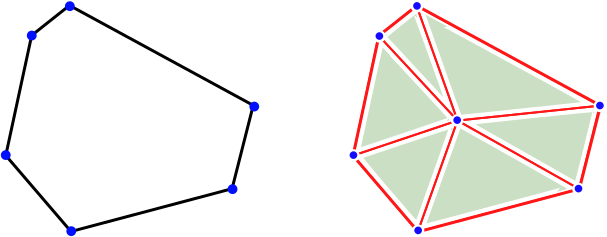
\includegraphics[width=3.5in]{figures/reproducing_element_shape.pdf}  \caption{A representative polygonal element and its corresponding edge-based partition.}
  \label{fig:reproducing_element_shape}
\end{figure}

For the partitioned element under consideration, the interpolation error of order $k=1$ for the CG-PEM was computed as $E_1 (\Omega) = 2.5465 \times 10^{-16}$ (on the order of machine precision). For the DG-PEM, the interpolation error was observed to be dependent upon the accuracy of the computations performed in solving (\ref{eq:dgpem_linear_system}). The log of $\kappa(\mathbf{J})$ provides a useful indicator of the number of digits of precision lost in computing $\mathbf{J}^{-1}$. This loss of precision is reflected by a corresponding increase in the interpolation error measure. Table \ref{tab:interpolation_error_and_condJ_k1} illustrates the connection between $E_1 (\Omega)$ and $\kappa(\mathbf{J})$ for various DG-PEM penalty parameter values. 

\begin{table}
\centering
\begin{subtable}{1.0\textwidth}
\centering
\begin{tabular}{| c || c | c | c | c |}
    \hline
DG-PEM & $\alpha_{\gamma0} = 10^{-3}$ & $\alpha_{\gamma0} = 10^{0}$ & $\alpha_{\gamma0} = 10^{3}$ & $\alpha_{\gamma0} = 10^{6}$ \\ \hline \hline
$\alpha_{\gamma1} = 0.0$	& 1.66E-013 & 7.48E-016 & 4.70E-014 & 1.79E-010 \\ \hline
$\alpha_{\gamma1} = 10^{0}$ & 1.65E-013 & 9.67E-016 & 8.73E-015 & 2.51E-011 \\ \hline
$\alpha_{\gamma1} = 10^{3}$ & 1.01E-012 & 2.66E-013 & 1.36E-015 & 4.49E-014 \\ \hline
$\alpha_{\gamma1} = 10^{6}$ & 1.13E-009 & 3.13E-010 & 7.10E-013 & 9.03E-016 \\
    \hline
    \end{tabular}
    \caption{Interpolation error: $E_1 (\Omega)$}
    \label{tab:interpolation_error_k1}
\end{subtable}% <---- don't forget this %
\\
\begin{subtable}{1.0\textwidth}
\centering
\begin{tabular}{| c || c | c | c | c |}
    \hline
DG-PEM & $\alpha_{\gamma0} = 10^{-3}$	&	$\alpha_{\gamma0} = 10^{0}$	&	$\alpha_{\gamma0} = 10^{3}$	&	$\alpha_{\gamma0} = 10^{6}$ \\ \hline \hline
$\alpha_{\gamma1} = 0.0$	&	5.44E+002 & 4.07E+000 & 5.94E+003 & 5.96E+006 \\ \hline
$\alpha_{\gamma1} = 10^{0}$	&	4.96E+003 & 2.01E+001 & 9.33E+002 & 9.29E+005 \\ \hline
$\alpha_{\gamma1} = 10^{3}$	&	1.58E+007 & 2.50E+004 & 6.96E+001 & 1.11E+003 \\ \hline
$\alpha_{\gamma1} = 10^{6}$	&	2.37E+010 & 2.50E+007 & 6.86E+004 & 6.98E+001 \\
    \hline
    \end{tabular}
    \caption{DG-PEM linear system conditioning: $\kappa(\mathbf{J})$}
    \label{tab:condJ_k1}
\end{subtable}

\caption{Computed values of $E_1 (\Omega)$ and $\kappa(\mathbf{J})$ for the element in Figure \ref{fig:reproducing_element_shape}, using various DG-PEM penalty parameter settings.}
\label{tab:interpolation_error_and_condJ_k1}
\end{table}

The results in table \ref{tab:interpolation_error_and_condJ_k1} confirm that $\mathbf{J}$ will become poorly conditioned if either of the two penalty parameters $\alpha_{\gamma0}$ or $\alpha_{\gamma1}$ are sufficiently large. This is true regardless of how the DG polynomial bases are specified within each geometric entity. Under certain circumstances, $\mathbf{J}$ will remain well-conditioned if both $\alpha_{\gamma0}$ and $\alpha_{\gamma1}$ are kept roughly proportional to one another, for all values of $\alpha_{\gamma0}, \, \alpha_{\gamma1} > 0$. If $\alpha_{\gamma0}$ and $\alpha_{\gamma1}$ are increased proportionally to one another, one recovers the behavior of the pure penalty DG-PEM in (\ref{eq:pure_penalty}).

It is remarked that other factors which impact with condition number of $\mathbf{J}$ may have detrimental effects on the accuracy of the element's interpolation error. Specifically, consider the case where the element in Figure \ref{fig:reproducing_element_shape} is scaled anisotropically by a factor of $0.01$ in the vertical direction, yielding a comparatively thin element with an aspect ratio of 100:1. For this element, the interpolation error using the CG-PEM increases only slightly, to $E_1 (\Omega) = 6.9817 \times 10^{-15}$. The corresponding values of $E_1 (\Omega)$ and $\kappa(\mathbf{J})$ for the DG-PEM are presented in table \ref{tab:thin_interpolation_error_and_condJ_k1}.

\begin{table}
\centering
\begin{subtable}{1.0\textwidth}
\centering
\begin{tabular}{| c || c | c | c | c |}
    \hline
DG-PEM & $\alpha_{\gamma0} = 10^{-3}$ & $\alpha_{\gamma0} = 10^{0}$ & $\alpha_{\gamma0} = 10^{3}$ & $\alpha_{\gamma0} = 10^{6}$ \\ \hline \hline
$\alpha_{\gamma1} = 0.0$	& 3.02E-014 & 9.01E-015 & 5.22E-013 & 1.59E-009 \\ \hline
$\alpha_{\gamma1} = 10^{0}$ & 3.99E-014 & 1.37E-014 & 2.02E-013 & 3.12E-012 \\ \hline
$\alpha_{\gamma1} = 10^{3}$ & 2.44E-011 & 6.48E-012 & 1.89E-012 & 3.34E-013 \\ \hline
$\alpha_{\gamma1} = 10^{6}$ & 1.52E-007 & 4.97E-008 & 1.85E-009 & 3.69E-012 \\
    \hline
    \end{tabular}
    \caption{Interpolation error: $E_1 (\Omega)$}
    \label{tab:thin_interpolation_error_k1}
\end{subtable}% <---- don't forget this %
\\
\begin{subtable}{1.0\textwidth}
\centering
\begin{tabular}{| c || c | c | c | c |}
    \hline
DG-PEM & $\alpha_{\gamma0} = 10^{-3}$	&	$\alpha_{\gamma0} = 10^{0}$	&	$\alpha_{\gamma0} = 10^{3}$	&	$\alpha_{\gamma0} = 10^{6}$ \\ \hline \hline
$\alpha_{\gamma1} = 0.0$	& 9.07E+003 & 1.39E+002 & 1.14E+005 & 1.33E+008 \\ \hline
$\alpha_{\gamma1} = 10^{0}$	& 3.52E+005 & 1.75E+003 & 1.97E+004 & 3.67E+005 \\ \hline
$\alpha_{\gamma1} = 10^{3}$	& 1.17E+009 & 2.46E+006 & 2.61E+005 & 2.32E+004 \\ \hline
$\alpha_{\gamma1} = 10^{6}$	& 1.77E+012 & 2.45E+009 & 2.52E+008 & 3.07E+005 \\
    \hline
    \end{tabular}
    \caption{DG-PEM linear system conditioning: $\kappa(\mathbf{J})$}
    \label{tab:thin_condJ_k1}
\end{subtable}

\caption{Computed values of $E_1 (\Omega)$ and $\kappa(\mathbf{J})$ for a comparatively thin element with an aspect ratio of 100:1, using various DG-PEM penalty parameter settings.}
\label{tab:thin_interpolation_error_and_condJ_k1}
\end{table}

Clearly, a careful selection of $\alpha_{\gamma0}$ and $\alpha_{\gamma1}$ is warranted for the sake of minimizing the resulting interpolation error. For general 2D applications in which an edge-based partitioning scheme is employed, it is suggested that the parameter values be chosen such that $\alpha_{\gamma0} = 10.0$ and $\alpha_{\gamma1} = 0.0$. However, it is recommended that a more thorough investigation be conducted to determine more optimal parameters settings for other element types.

\section{Finite Element Patch Tests}

In this section we investigate the behavior of PEM elements in the context of the classical patch test introduced by Irons in the Appendix of \cite{Irons:65}, whose passage is argued in \cite{Simo&Taylor:86} to be a necessary and sufficient condition for convergence. This claim has been disputed, namely by Stummel in \cite{Stummel:80}. Nonetheless, it serves as a useful indicator for the expected convergence properties of conforming finite elements. Two tests will be considered: the linear and quadratic patch tests, as depicted in figure \ref{fig:polygonal_patches}.

\begin{figure}[!h]
    \centering
    \begin{subfigure}[b]{0.49\linewidth}
            \centering
            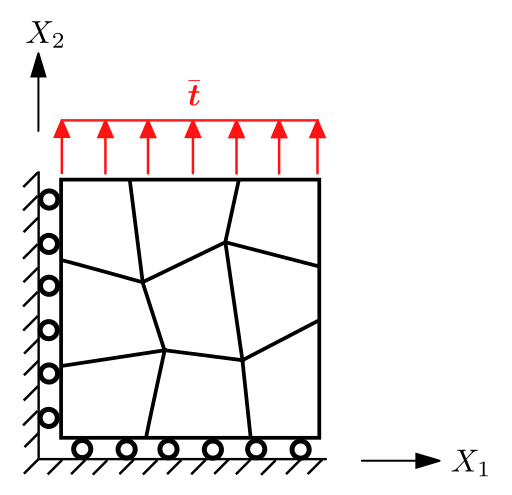
\includegraphics[width=2.5in]{figures/linear_patch_test.pdf}
    			\caption{linear patch test \label{fig:linear_patch_test}}
    \end{subfigure}
	\begin{subfigure}[b]{0.49\linewidth}
            \centering
            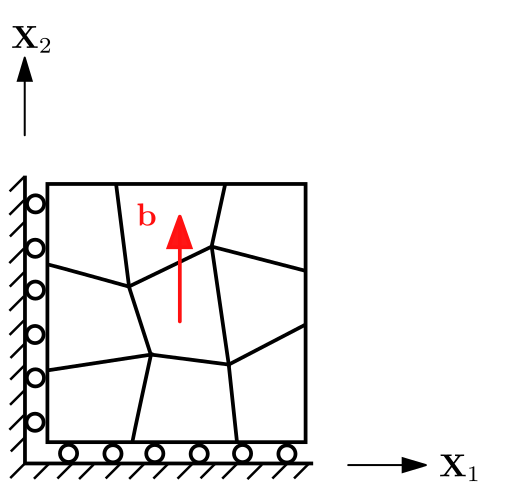
\includegraphics[width=2.5in]{figures/quadratic_patch_test.pdf}
    			\caption{quadratic patch test \label{fig:quadratic_patch_test}}
    \end{subfigure}
    \caption{Depiction of simple patch tests for (\subref{fig:linear_patch_test}) linear and (\subref{fig:quadratic_patch_test}) quadratic elements.}
    \label{fig:polygonal_patches}
\end{figure}

The linear patch test consists of a square patch of elements with dimensions $L \times L$. The normal components of displacement on the $-X_1$ and $-X_2$ faces of the patch are constrained such that
\begin{equation}
	u_1 (X_1 = 0) = 0, \quad u_2 (X_2 = 0) = 0.
\end{equation}
A constant vertical traction $\bar{\mathbf{t}} = (0, \, T)$ is prescribed on the $+X_2$ face of the patch. For a linear elastic body under plane strain conditions, an exact solution for the in-plane displacement and stress fields is easily obtained:
\begin{equation}
	u_1 (\mathbf{X}) = - \frac{\nu}{2 \mu} T X_1, \quad u_2 (\mathbf{X}) = \frac{(1-\nu)}{2 \mu} T X_2,
\end{equation}
\begin{equation}
	\sigma_{11} (\mathbf{X}) = \sigma_{12} (\mathbf{X}) = 0, \quad \sigma_{22} (\mathbf{X}) = T.
\end{equation}

For the quadratic patch test, we will consider a similarly constrained square patch as for the linear patch test. A constant body force $\mathbf{b} = (b_1, \, b_2)$ acts uniformly over the patch. Additionally, linearly varying tractions are applied to the unconstrained faces of the patch:
\begin{equation}
	\bar{t}_1 (X_1 = L) = - \frac{\lambda}{\lambda + 2 \mu} b_2 X_2, \quad \bar{t}_2 (X_1 = L) = 0,
\end{equation}
\begin{equation}
	\bar{t}_2 (X_2 = L) = - \frac{\lambda}{\lambda + 2 \mu} b_1 X_2, \quad \bar{t}_1 (X_2 = L) = 0.
\end{equation}
For a linear elastic material under plane strain conditions, an exact solution may be obtained of the form:
\begin{equation}
	u_1 (\mathbf{X}) = \frac{b_1}{2 (\lambda + 2 \mu)} (L - X_1) X_1 + \frac{\nu (b_1 - b_2)}{2 \mu} L X_1,
\end{equation}
\begin{equation}
	u_2 (\mathbf{X}) = \frac{b_2}{2 (\lambda + 2 \mu)} (L - X_2) X_2 + \frac{\nu (b_2 - b_1)}{2 \mu} L X_2,
\end{equation}
\begin{equation}
	\sigma_{11} (\mathbf{X}) = b_1 (L - X_1) + \frac{\lambda}{\lambda + 2 \mu} b_2 X_2,
\end{equation}
\begin{equation}
	\sigma_{22} (\mathbf{X}) = b_2 (L -  X_2) + \frac{\lambda}{\lambda + 2 \mu} b_1 X_1,
\end{equation}
\begin{equation}
	\sigma_{12} (\mathbf{X}) = 0.
\end{equation}
A simplistic uniaxial case involving only a constant body force and no boundary tractions occurs when $\nu = 0$ and $b_1 = 0$:
\begin{equation}
	u_1 (\mathbf{X}) = 0, \quad u_2 (\mathbf{X}) = \frac{b_2}{2 (\lambda + 2 \mu)} (L - X_2) X_2,
\end{equation}
\begin{equation}
	\sigma_{11} (\mathbf{X}) = \sigma_{12} (\mathbf{X}) = 0, \quad \sigma_{22} (\mathbf{X}) = b_2 (L -  X_2).
\end{equation}

Patch test errors were measured in terms of the normalized $L^2 (\Omega)$ error metrics for displacement and stress:
\begin{equation}
	\frac{||\mathbf{u}^h - \mathbf{u}||}{||\mathbf{u}||} = \sqrt{\frac{\int_{\mathcal{B}_0} (\mathbf{u}^h - \mathbf{u}) \cdot (\mathbf{u}^h - \mathbf{u}) \, dV}{\int_{\mathcal{B}_0} \mathbf{u} \cdot \mathbf{u} \, dV}},
\end{equation}
\begin{equation}
	\frac{||\boldsymbol{\sigma}^h - \boldsymbol{\sigma}||}{||\boldsymbol{\sigma}||} = \sqrt{\frac{\int_{\mathcal{B}_0} (\boldsymbol{\sigma}^h - \boldsymbol{\sigma}) \colon (\boldsymbol{\sigma}^h - \boldsymbol{\sigma}) \, dV}{\int_{\mathcal{B}_0} \boldsymbol{\sigma} \colon \boldsymbol{\sigma} \, dV}},
	\label{eq:normalized_stress_error}
\end{equation}
where $\mathbf{u}$ and $\boldsymbol{\sigma}$ denote the exact solutions for the displacement and stress fields, respectively.

\subsection*{Linear Patch Tests in 2D}

The two meshes depicted in Figure \ref{fig:patch_test_meshes} are considered. The PEM was used on the polygonal mesh, whereas the FEM with standard 4-nodes isoparametric elements was used on the quadrilateral mesh.

\begin{figure}[!h]
    \centering
    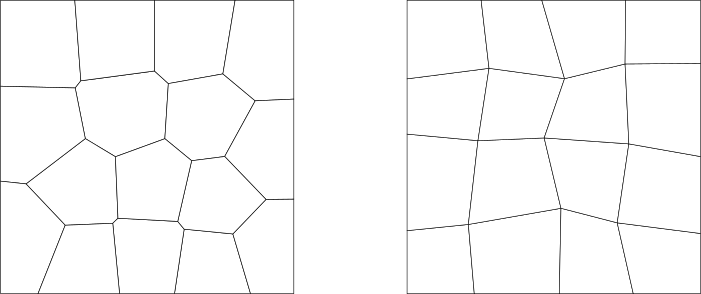
\includegraphics[width=4.0in]{figures/patch_test_meshes.pdf}
    	\caption{Meshes used for the linear patch test: (left) polygonal mesh, (right) distorted quadrilateral mesh.}
    \label{fig:patch_test_meshes}
\end{figure}

Linear patch test errors for the FEM, CG-PEM, and DG-PEM were explored. Both the CG-PEM and DG-PEM utilized an edge-based partitioning scheme and composite mid-point quadrature rules for each element. Unless otherwise noted, the parameters for the DG-PEM were selected as $\epsilon = +1$, $\alpha_{\gamma0} = 10.0$, and $\alpha_{\gamma1} = 0.0$. Further, the DG-PEM was tested both with and without using the gradient correction scheme presented in \cite{Talischi:15}. These corrections were applied to the test function gradients alone (yielding a ``nonsymmetric correction'' scheme), or to both the trial and test function gradients (yielding a ``symmetric correction'' scheme). The results of these tests may be found in table \ref{tab:linear_patch_test}.

\begin{table}[!ht]
  \begin{center}
    \begin{tabular}{| c || c | c |}
    \hline
           & $||\mathbf{u}^h - \mathbf{u}|| / ||\mathbf{u}||$ & $||\boldsymbol{\sigma}^h - \boldsymbol{\sigma}|| / ||\boldsymbol{\sigma}||$ \\ \hline \hline
    FEM (4-node quadrilaterals) & 5.1568E-015 & 7.7395E-016 \\ \hline
    CG-PEM (no gradient correction) & 5.9125E-012 & 5.1637E-012 \\ \hline
    DG-PEM (no gradient correction) & 2.7721E-005 & 3.0904E-004 \\ \hline
    DG-PEM (symmetric correction) & 6.2750E-012 & 5.3521E-012 \\ \hline
    DG-PEM (nonsymmetric correction) & 6.2673E-012 & 5.3494E-012 \\
    \hline
    \end{tabular}
    \caption{Linear patch test results comparison for FEM, CG-PEM, and DG-PEM.}
    \vspace{-5pt}
    \label{tab:linear_patch_test}
    \vspace{-25pt}
  \end{center}
\end{table}

The classical FEM produces errors on the order of machine precision. The CG-PEM produces results that are only slightly less accurate. As expected, the errors for the CG-PEM are unaffected by the use (or disuse) of a gradient correction scheme. In contrast, the DG-PEM produces noticeable errors if no gradient correction scheme is employed. Using either of the symmetric or nonsymmetric gradient correction schemes with the DG-PEM yields comparable accuracy to the CG-PEM.

These observations help to illuminate an important point regarding the consistent integration of the weak form. Consider the consistency equations in (\ref{eq:consistency}). It is remarked that any continuous field $\varphi_a \in C^0 (\Omega_e)$ integrated exactly in (\ref{eq:consistency}) will lead to direct satisfaction of quadrature consistency. Such is the case for the CG-PEM under the present circumstances. However, if $\varphi_a$ is not a continuous field, neither (\ref{eq:consistency}) nor quadrature consistency will be satisfied, in general. Such is the case for the DG-PEM, even when exact integration is used. The consequence is violation of patch tests. This can be mitigated through the use of a gradient correction scheme, or alternatively through an appropriate selection of the DG-PEM parameters. Specifically, in the limit as $\alpha_{\gamma0} \rightarrow \infty$, the DG-PEM reduces to the CG-PEM, and the resulting patch test errors can be eliminated. Table \ref{tab:linear_patch_test_parameter_study} demonstrates this behavior for increasing values of $\alpha_{\gamma0}$, in the absence of a gradient correction scheme.

\begin{table}[!ht]
  \begin{center}
    \begin{tabular}{| c || c | c | c | c | c |}
    \hline
    DG-PEM & $\alpha_{\gamma0} = 10^{-6}$ & $\alpha_{\gamma0} = 10^{-3}$ & $\alpha_{\gamma0} = 10^{0}$ & $\alpha_{\gamma0} = 10^{3}$ & $\alpha_{\gamma0} = 10^{6}$ \\ \hline \hline
    	$\alpha_{\gamma1} = 0.0$ & 2.8433E-009 & 2.8152E-006 & 3.3114E-004 & 4.8035E-006 & 4.8278E-009 \\ \hline
    $\alpha_{\gamma1} = 10^{-3}$ & 2.8505E-009 & 2.8224E-006 & 3.2288E-004 & 4.9805E-006 & 5.0082E-009 \\ \hline
    $\alpha_{\gamma1} = 10^{0}$ & 3.4853E-009 & 3.4604E-006 & 2.4827E-003 &  7.4284E-004 & 8.6376E-007 \\ \hline
    $\alpha_{\gamma1} = 10^{3}$ & 3.5460E-009 & 3.5450E-006 & 3.0047E-003 & 1.3898E-002 & 7.4705E-004 \\ \hline
    $\alpha_{\gamma1} = 10^{6}$ & 3.5457E-009 & 3.5456E-006 & 3.0054E-003 & 1.4604E-002 & 1.3953E-002 \\
    \hline
    \end{tabular}
    \caption{Computed values of $||\boldsymbol{\sigma}^h - \boldsymbol{\sigma}|| / ||\boldsymbol{\sigma}||$ for the DG-PEM using various penalty parameter settings. No gradient correction scheme was utilized. Identical trends were observed for $||\mathbf{u}^h - \mathbf{u}|| / ||\mathbf{u}||$.}
    \vspace{-5pt}
    \label{tab:linear_patch_test_parameter_study}
    \vspace{-25pt}
  \end{center}
\end{table}

Additionally, it is noted that the DG-PEM recovers integration consistency in the limit as $\alpha_{\gamma0} \rightarrow 0$. This is a direct consequence of (\ref{eq:weak_compatibility_enforcement}). It is tempting to want to specify $\alpha_{\gamma0}$ to be sufficiently small/large enough to reduce patch test errors to an acceptable level. However, this thinking must be tempered by an understanding of the effects of interpolation error on patch test errors. Recall that the interpolation error $E_1 (\Omega)$ for a given element is controlled largely by the conditioning of $\mathbf{J}$. In turn, $\kappa (\mathbf{J})$ will be adversely affected by sufficiently small/large values of $\alpha_{\gamma0}$. Table \ref{tab:interpolation_patch_test_error} demonstrates the consequent limitations imposed upon the choice of $\alpha_{\gamma0}$ due to excessive interpolation error.

\begin{table}[!ht]
  \begin{center}
    \begin{tabular}{| c || c | c | c | c |}
    \hline
    DG-PEM & $\kappa(\mathbf{J})$ &  $E_1 (\Omega)$ & $||\mathbf{u}^h - \mathbf{u}|| / ||\mathbf{u}||$ & $||\boldsymbol{\sigma}^h - \boldsymbol{\sigma}|| / ||\boldsymbol{\sigma}||$ \\ \hline \hline
    $\alpha_{\gamma0} = 10^{0}$ & 4.3653E+000 & 3.7339E-015 & 3.9872E-005 & 3.3113E-004 \\ \hline
    $\alpha_{\gamma0} = 10^{3}$ & 6.1670E+003 & 2.5645E-012 & 3.5373E-007 & 4.8035E-006 \\ \hline
    $\alpha_{\gamma0} = 10^{6}$ & 6.1816E+006 & 2.2129E-009 & 3.5767E-010 & 4.8276E-009 \\ \hline
    $\alpha_{\gamma0} = 10^{9}$ & 6.1817E+009 & 1.6471E-006 & 1.4331E-009 & 2.4472E-008 \\ \hline
    $\alpha_{\gamma0} = 10^{12}$ & 6.1821E+012 & 1.7678E-003 & 2.1612E-006 & 3.0495E-005 \\
    \hline
    \end{tabular}
    \caption{The effects of interpolation error on patch test errors in the DG-PEM. No gradient correction scheme was utilized.}
    \vspace{-5pt}
    \label{tab:interpolation_patch_test_error}
    \vspace{-25pt}
  \end{center}
\end{table}

If the interpolation error $E_1 (\Omega)$ becomes large enough (due to poor conditioning of $\mathbf{J}$), it will dominate any other sources of error incurred in the patch test. Moreover, interpolation errors persist even if a gradient correction scheme is employed, and can become particularly troublesome for: thin elements, higher-order elements, or elements with nearly degenerate features.

\subsection*{Linear Patch Tests in 3D}

For the linear patch test described in the previous example, a fairly straightforward extension to the case of 3-dimensions is obtained by considering a cube of dimensions $L \times L \times L$ with normal displacements constrained on its $-X_1$, $-X_2$, and $-X_3$ faces:
\begin{equation}
	u_1 (X_1 = 0) = 0, \quad u_2 (X_2 = 0) = 0, \quad u_3 (X_3 = 0) = 0.
\end{equation}
A constant vertical traction $\bar{\mathbf{t}} = (0, \, 0, \, T)$ is prescribed on the $+X_3$ face of the patch. For a linear elastic body, the exact solution is:
\begin{equation}
	u_1 (\mathbf{X}) = - \frac{\nu}{E} T X_1, \quad u_2 (\mathbf{X}) = - \frac{\nu}{E} T X_2, \quad u_3 (\mathbf{X}) = \frac{T}{E} X_3, 
\end{equation}
\begin{equation}
	\sigma_{33} (\mathbf{X}) = T, \quad \text{all other } \sigma_{ij} (\mathbf{X}) = 0.
\end{equation}

%A curious set of results are obtained for polyhedral elements. Specifically, the DG-PEM elements do not pass patch tests, even if a gradient correction scheme is applied. This can be explained by virtue of the DG-PEM's lack of continuity/consistency in the representation of $\varphi^h \in \partial \Omega$. Because 2D DG-PEM elements typically have continuous representations for $\varphi^h|_{\partial \Omega} \in C^0 (\partial \Omega)$, we may directly apply a gradient correction scheme in such cases, yielding satisfaction of patch tests. However, for 3D DG-PEM elements, this is not the case. Rather, $\varphi^h|_{\partial \Omega} \not \in C^0 (\partial \Omega)$, and we cannot guarantee the necessary conditions to pass patch tests (i.e. we lack ``weak compatibility''). However, in the limit as $\alpha_{\gamma0} \rightarrow \infty$ ($\alpha_{\gamma1}$ small), we recover a $C^0 (\partial \Omega)$ representation for $\varphi^h|_{\partial \Omega}$, leading to satisfaction of finite element patch tests. A few numerical tests support this hypothesis. This suggests that use of the CG-PEM on $\partial \Omega$ may be the best course of action. Subsequently, the DG-PEM may be used on the interior of $\Omega$ with impunity. Alternatively, one would need to enforce some additional set of constraints on each face to guarantee ``weak compatibility.''

The two hexahedral meshes depicted in Figure \ref{fig:hexahedral_patch_meshes} were used in conjunction with the FEM, whereas the DG-PEM was used on the polyhedral mesh depicted in Figure \ref{fig:polyhedral_patch_mesh}. The DG-PEM parameter settings were consistent with those used for the 2D patch test. The results are displayed in Table \ref{tab:linear_patch_test_3d}.

\begin{figure}[!h]
    \centering
    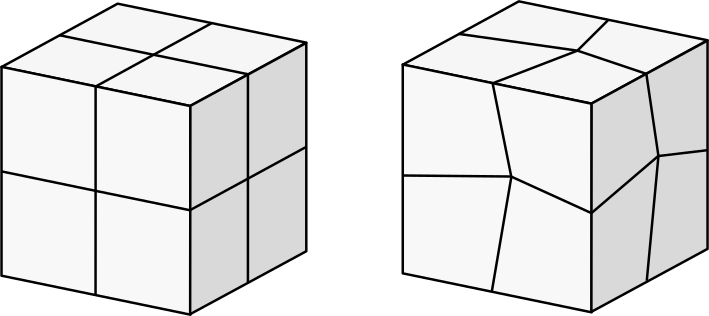
\includegraphics[width=4.0in]{figures/hexahedral_patch_meshes.pdf}
    	\caption{Hexahedral meshes: (left) regular, (right) distorted.}
    \label{fig:hexahedral_patch_meshes}
\end{figure}

\begin{figure}[!h]
    \centering
    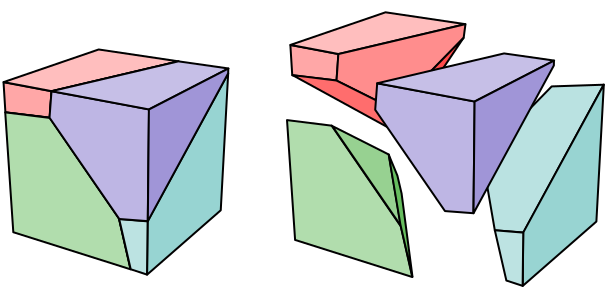
\includegraphics[width=4.0in]{figures/polyhedral_patch_mesh.pdf}
    	\caption{Patch of polyhedral elements.}
    \label{fig:polyhedral_patch_mesh}
\end{figure}

\begin{table}[!ht]
  \begin{center}
    \begin{tabular}{| c || c | c | c |}
    \hline
           & $E_1 (\Omega)$ & $||\mathbf{u}^h - \mathbf{u}|| / ||\mathbf{u}||$ & $||\boldsymbol{\sigma}^h - \boldsymbol{\sigma}|| / ||\boldsymbol{\sigma}||$ \\ \hline \hline
    FEM (regular hexahedra) & 2.4441E-016 & 1.5371E-015 & 8.1102E-016 \\ \hline
    FEM (distorted hexahedra) & 3.4394E-016 & 7.5402E-011 & 1.6047E-010 \\ \hline
    DG-PEM (no gradient correction) & 2.0369E-008 & 2.7189E-001 & 4.4846E-001 \\ \hline
    DG-PEM (symmetric correction) & 4.1522E-008 & 1.2598E-008 & 4.1608E-008 \\ \hline
    DG-PEM (nonsymmetric correction) & 2.0369E-008 & 1.0193E-008 & 2.9253E-008 \\
    \hline
    \end{tabular}
    \caption{3D linear patch test results comparison for FEM and DG-PEM.}
    \vspace{-5pt}
    \label{tab:linear_patch_test_3d}
    \vspace{-25pt}
  \end{center}
\end{table}

It is interesting to note that the FEM incurs a mild amount of error on the distorted hexahedral mesh. Given that the elements' interpolation error remains unchanged, this error is partially attributable to inaccuracies in the numerical integration used for the elements. Using higher-order Gaussian product rules on the isoparametric elements and their faces reduces the patch test errors to a certain extent, but nonetheless, some residual errors still remain.

In contrast, the accuracy of the DG-PEM appears to be limited more by interpolation error. As before, these errors are attributable to poor conditioning of the DG-PEM systems of equations. The current evidence suggests that the conditioning of $\mathbf{J}$ becomes worse in higher spatial dimensions. The use of either the symmetric or nonsymmetric gradient correction scheme assists in restoring integration consistency, yielding patch test errors on the order of $E_1 (\Omega)$.

\subsection*{Quadratic Patch Tests in 2D}

The two quadrilateral meshes depicted in Figure \ref{fig:quadrilateral_patch_meshes} were used in conjunction with the FEM, using both 8-node serendipity and 9-node Lagrange isoparametric formulations. The PEM was used on the polygonal mesh depicted in Figure \ref{fig:quadratic_polygonal_patch_mesh}.

\begin{figure}[!h]
    \centering
    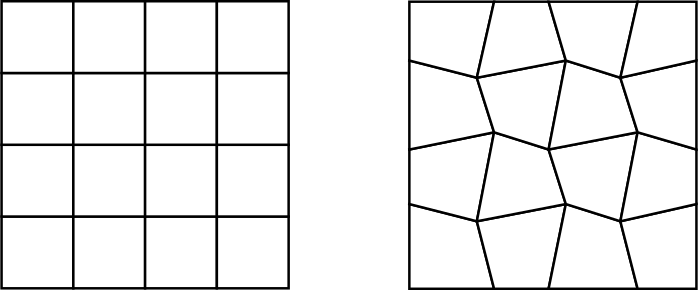
\includegraphics[width=4.0in]{figures/quadrilateral_patch_meshes.pdf}
    	\caption{Quadrilateral meshes: (left) regular, (right) distorted.}
    \label{fig:quadrilateral_patch_meshes}
\end{figure}

\begin{figure}[!h]
    \centering
    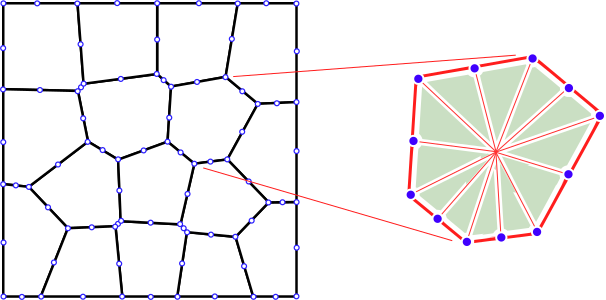
\includegraphics[width=4.0in]{figures/quadratic_polygonal_patch_mesh.pdf}
    	\caption{Patch of serendipity polygonal elements.}
    \label{fig:quadratic_polygonal_patch_mesh}
\end{figure}

Quadratic patch test errors for the FEM and DG-PEM were explored. The DG-PEM utilized an edge-based partitioning scheme and composite mid-point quadrature rules for each element. The DG-PEM bases was chosen such that $\varphi^h \in \mathcal{D}^h_2 (\Omega)$, yielding quadratically complete shape functions. Further, the DG-PEM was tested both with and without using the symmetric and nonsymmetric gradient correction schemes discussed previously. The results are presented in table \ref{tab:quadratic_patch_test}.

\begin{table}[!ht]
  \begin{center}
    \begin{tabular}{| c || c | c | c |}
    \hline
           & $E_2 (\Omega)$ & $||\mathbf{u}^h - \mathbf{u}|| / ||\mathbf{u}||$ & $||\boldsymbol{\sigma}^h - \boldsymbol{\sigma}|| / ||\boldsymbol{\sigma}||$ \\ \hline \hline
    FEM (regular 8-node quadrilaterals) & 9.0812E-016 & 1.7437E-009 & 1.3950E-008 \\ \hline
    FEM (distorted 8-node quadrilaterals) & 4.7831E-003 & 9.9714E-005 & 2.0795E-003 \\ \hline
    FEM (regular 9-node quadrilaterals) & 8.6713E-016 & 1.7437E-009 & 1.3950E-008 \\ \hline
    FEM (distorted 9-node quadrilaterals) & 1.2818E-015 & 2.0841E-009 & 1.5752E-008 \\ \hline
    DG-PEM (no gradient correction) & 3.3857E-008 & 9.8535E-002 & 2.8876E-001 \\ \hline
    DG-PEM (symmetric correction) & 3.6486E-007 & 3.5935E-008 & 1.4642E-007 \\ \hline
    DG-PEM (nonsymmetric correction) & 3.3857E-008 & 4.5498E-009 & 5.5341E-009 \\
    \hline
    \end{tabular}
    \caption{Quadratic patch test results comparison for FEM and DG-PEM.}
    \vspace{-5pt}
    \label{tab:quadratic_patch_test}
    \vspace{-25pt}
  \end{center}
\end{table}

It is interesting to note that the 8-node isoparametric quadrilaterals fail the quadratic patch test if the mesh becomes distorted. Only affinely distorted quadrilaterals of this type will exhibit quadratic completeness. Arbitrarily distorted elements will suffer from excessive interpolation errors, as observed in Table \ref{tab:quadratic_patch_test}. This behavior is discussed in greater detail in \cite{Arnold:02} and \cite{Arnold:01}. In comparison, the 9-node quadrilateral elements preserve quadratic completeness, even when distorted as in Figure \ref{fig:quadrilateral_patch_meshes}. However, it should be remarked that if the elements' edges are curved, both the 8- and 9-node isoparametric elements will lose 2nd order completeness and fail quadratic patch tests.

To account for the effects of integration error, the DG-PEM requires the use of a gradient correction scheme. However, if a symmetric correction scheme is employed, it is observed that there is a loss of completeness in the representation of the solution gradients over the element, corresponding to an increase in the interpolation error. Only the nonsymmetric gradient correction method is able to achieve the desired level of accuracy in the quadratic patch test. It shall therefore be used exclusively throughout the remainder of our discussions.

\subsection*{Quadratic Patch Tests in 3D}

The quadratic patch test described in the previous example may be extended directly to the 3-dimensional setting. As for the 3D linear patch test, the two hexahedral meshes depicted in Figure \ref{fig:hexahedral_patch_meshes} were used in conjunction with the FEM, this time using 20-node isoparametric elements. The DG-PEM was used on the ``serendipity'' polyhedral mesh depicted in Figure \ref{fig:quadratic_polyhedral_patch_mesh}, with similar parameter settings to those used for the 2D patch test. The results are displayed in Table \ref{tab:quadratic_patch_test_3d}.

\begin{figure}[!h]
    \centering
    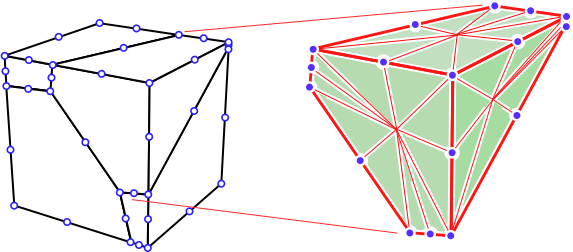
\includegraphics[width=4.0in]{figures/quadratic_polyhedral_patch_mesh.pdf}
    	\caption{Patch of serendipity polyhedral elements.}
    \label{fig:quadratic_polyhedral_patch_mesh}
\end{figure}

\begin{table}[!ht]
  \begin{center}
    \begin{tabular}{| c || c | c | c |}
    \hline
           & $E_2 (\Omega)$ & $||\mathbf{u}^h - \mathbf{u}|| / ||\mathbf{u}||$ & $||\boldsymbol{\sigma}^h - \boldsymbol{\sigma}|| / ||\boldsymbol{\sigma}||$ \\ \hline \hline
    FEM (regular hexahedra) & 6.1677E-016 & 6.9751E-009 & 2.7900E-008 \\ \hline
    FEM (distorted hexahedra) & 5.6085E-003 & 1.4755E-004 & 1.4958E-003 \\ \hline
    DG-PEM (no gradient correction) & 3.2351E-008 & 1.3054E-001 & 2.9833E-001 \\ \hline
    DG-PEM (symmetric correction) & 9.7520E-002 & 2.4536E-002 & 3.1112E-002 \\ \hline
    DG-PEM (nonsymmetric correction) & 3.2351E-008 & 2.6577E-008 & 1.1622E-008 \\
    \hline
    \end{tabular}
    \caption{3D quadratic patch test results comparison for FEM and DG-PEM.}
    \vspace{-5pt}
    \label{tab:quadratic_patch_test_3d}
    \vspace{-25pt}
  \end{center}
\end{table}

As was the case in 2D, the 20-node isoparametric brick elements perform well on the regular (undistorted) mesh, but lose polynomial completeness on the distorted mesh. Correspondingly, there is an observed loss of accuracy in both $E_2 (\Omega)$ and the patch test error metrics.

For the DG-PEM elements, we observe an interesting phenomenon with respect to the choice of gradient correction scheme. Under the present circumstances, applying a symmetric gradient correction (to both the trial and test functions) adversely impacts the polynomial completeness properties of the trial solution space. This result highlights the particular advantage of the nonsymmetric gradient correction scheme, which only modifies the test functions. Polynomial completeness of the trial solution space is therefore preserved, and patch test errors are rendered comparable with the (undistorted) FEM.

%Another quadratic patch test which involves no body force considers an elastic cantilever beam in pure bending, as depicted in Figure \ref{fig:bending_patch_test}. For clarity, this problem shall be referred to as the ``bending patch test.'' The support conditions of the (weakly) fixed beam are
%\begin{equation}
%	u_1 (X_1 = 0) = 0, \quad u_2 (X_1 = 0, X_2 = 0) = 0.
%\end{equation}
%A linearly varying traction $\bar{\mathbf{t}} = (M X_2, \, 0)$ is applied to the free end of the beam. For plane strain isotropic elasticity, the exact solution is:
%\begin{equation}
%	u_1 (\mathbf{X}) = \frac{M (\lambda + 2 \mu)}{4 \mu (\lambda + \mu)} X_1 X_2,
%\end{equation}
%\begin{equation}
%	u_2 (\mathbf{X}) = - \frac{M}{8 \mu (\lambda + \mu)} \left[ (\lambda + 2 \mu) X_1^2 + \lambda X_2^2 \right],
%\end{equation}
%\begin{equation}
%	\sigma_{11} = M X_2, \quad \sigma_{22} = \sigma_{12} = 0.
%\end{equation}

\section{Tests for Element Quality}

\subsection*{Conditioning of Individual Element Stiffness Matrices}

Partitioned element methods allow for the elements to take on virtually arbitrary shape. Nonetheless, elements with non-convex or degenerate features may degrade the overall accuracy of the resulting numerical solution. This section attempts to characterize the behavior of a representative sampling of polygonal PEM elements by examining the eigenvalues of each element's elastic stiffness matrix.

The motivation for the present study is to assess the effects of element formulation upon a given element's susceptibility to geometric locking phenomena. Heuristically: an element will be more sensitive to the effects of locking if its local stiffness matrix contains a number of eigenmodes (modes of deformation) whose corresponding eigenvalues are excessively large in comparison with the low-order deformation modes.

As a separate issue from locking, if a given element's local stiffness matrix is poorly conditioned, the global stiffness matrix of a mesh which contains said element may become poorly conditioned, as well. This may negatively impact the degree of solution accuracy that can be obtained due to floating point arithmetic. For implicit solid mechanics applications, the accuracy of any linear solver (whether direct or iterative) will be compromised by poor conditioning of the global stiffness matrix.

For the elements considered, a comparison study was carried out to examine differences in the eigenvalue spectra of elements whose stiffness matrices were computed using various element formulations. Specifically, approximations to harmonic shape functions were obtained for each element using the VETFEM, the CG-PEM, and the DG-PEM. These results were compared against a computed reference solution for the harmonic shape functions.

For each element, the elastic constants for Young's modulus and Poisson's ratio were chosen as $E = 1.0$ and $\nu = 0.0$, respectively. The choice of $\nu = 0.0$ is deliberate, and aims to decouple the effects of volumetric locking from the effects of geometric locking. All elements were scaled to have roughly unit diameter.

\subsubsection*{Examination of the Effects of Geometric Non-convexity}

A study was carried out to assess the effects of geometric non-convexity on a given element's eigenvalue spectrum. Three element shapes were considered, including: (A) a regular convex polygon, (B) an element with two collinear edges, and (C) a non-convex polygon. These elements are illustrated in Figure \ref{fig:concave_element_shapes}.

\begin{figure}[!h]
  \centering
  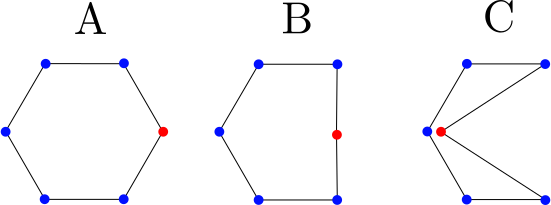
\includegraphics[width=3.5in]{figures/concave_element_shapes.pdf}  \caption{A representative sampling of hexagonal elements: (A) strictly convex, (B) two collinear edges, (C) non-convex.}
  \label{fig:concave_element_shapes}
\end{figure}

The harmonic shape functions defined on these elements were approximated using the VETFEM, the CG-PEM, and the DG-PEM. The VETFEM approximations consisted of 4th order polynomials, and were obtained as the solutions to (\ref{eq:vetfem}). The CG-PEM and DG-PEM approximations were obtained using the random Delaunay partitions shown in Figure \ref{fig:concave_element_partitions}. The penalty parameters appearing in (\ref{eq:penalty_parameters}) for the DG-PEM were chosen such that $\alpha_{\gamma0} = 10$, $\alpha_{\gamma1} = 0$ for all segments $\gamma$. Unless otherwise noted, the NIPG version of the DG-PEM (with $\epsilon = +1$) was utilized throughout. Reference solutions for the harmonic shape functions were computed on a highly refined partition of the element using the CG-PEM.

\begin{figure}[!h]
  \centering
  
\includegraphics[width=3.5in]{figures/concave_element_partitions.pdf}  \caption{Delaunay partitions for elements A, B, and C.}
  \label{fig:concave_element_partitions}
\end{figure}

For the red nodes indicated in Figure \ref{fig:concave_element_shapes}, color plots of the associated harmonic shape functions (and their corresponding approximations) are provided in Figure \ref{fig:concave_element_comparison}.

\begin{figure}[!h]
  \centering
  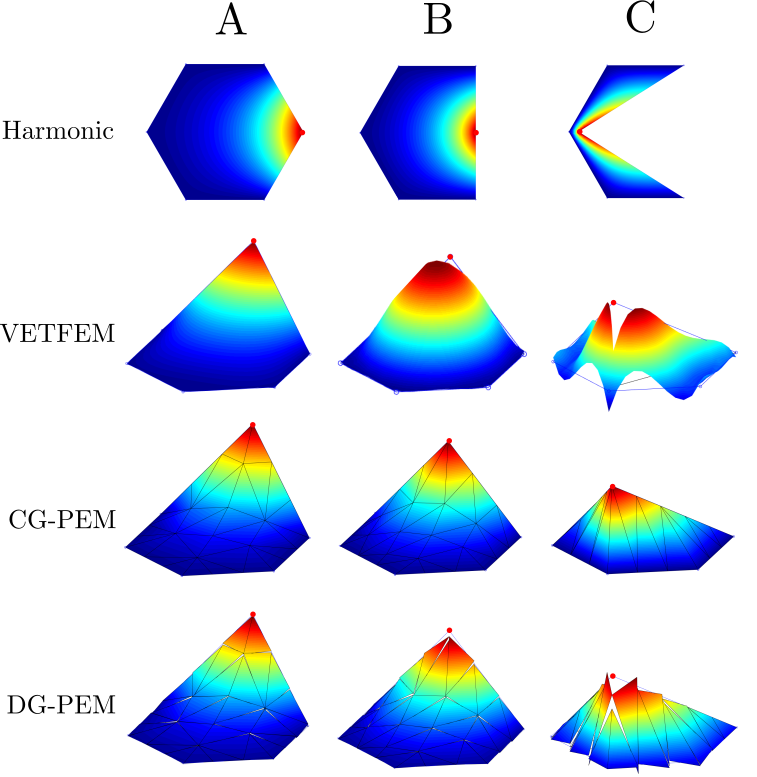
\includegraphics[width=5.0in]{figures/concave_element_comparison.pdf}  \caption{Comparison of the shape functions computed for elements A, B, and C using the VETFEM, CG-PEM, and DG-PEM.}
  \label{fig:concave_element_comparison}
\end{figure}

Concerning the VETFEM approximations depicted in Figure \ref{fig:concave_element_comparison} (particularly for elements B and C), the resulting shape functions present a number of undesirable features: oscillations, non-positivity, and non-interpolatory behavior. By comparison, the DG-PEM approximations avoid the issue of oscillations, though they are not strictly positive, nor are they interpolatory. Only the CG-PEM approximations can claim good behavior on all three fronts: they are non-oscillatory, strictly positive, and interpolatory. Nonetheless, it is important to emphasize that the aforementioned properties are not strictly necessary for convergence of the overall method. So long as a stable and consistent integration of the weak form is obtained, convergence is achieved. For certain applications, maintaining strict positivity or continuity of the shape function approximations may be desirable, though such applications are not considered here.

Using the aforementioned approximations in place of the harmonic shape functions, the elements' elastic stiffness matrices were computed (by numerical quadrature). The eigendecomposition of each element's local stiffness matrix was then determined, with particular attention paid to the largest eigenvalue $\lambda_{\max}$ and the smallest (non-zero) eigenvalue $\lambda_{\min}$. A comparison of the computed values for $\lambda_{\max}$ and $\lambda_{\min}$ is provided in table \ref{tab:concave_stiffness_max_min_eigenvalue}.

\begin{table}
\centering
\begin{subtable}{.5\textwidth}
\centering
\begin{tabular}{| c || c | c | c |}
    \hline
		Element  & A      & B      & C \\ \hline \hline
		Harmonic	 & 0.9635 & 1.2151 & 7.1166 \\ \hline
		VETFEM	 & 0.9950 & 4.4864 & 6.0305 \\ \hline
		CG-PEM	 & 1.0723 & 1.2760 & 8.7108 \\ \hline
		DG-PEM	 & 0.9668 & 1.1997 & 6.2766 \\
    \hline
    \end{tabular}
    \caption{Largest eigenvalue: $\lambda_{\max}$}
    \label{tab:concave_stiffness_max_eigenvalue}
\end{subtable}% <---- don't forget this %
\begin{subtable}{.5\textwidth}
\centering
\begin{tabular}{| c || c | c | c |}
    \hline
		Element  & A      & B      & C \\ \hline \hline
		Harmonic	 & 0.5226 & 0.3449 & 0.00562 \\ \hline
		VETFEM   & 0.5335 & 0.3491 & 0.09189 \\ \hline
		CG-PEM   & 0.6175 & 0.3935 & 0.00694 \\ \hline
		DG-PEM   & 0.5345 & 0.3425 & 0.00527 \\
    \hline
    \end{tabular}
    \caption{Smallest (non-zero) eigenvalue: $\lambda_{\min}$}
    \label{tab:concave_stiffness_min_eigenvalue}
\end{subtable}

\caption{Comparison of maximum and minimum (non-zero) eigenvalues of the element stiffness matrices for the elements shown in Figure \ref{fig:concave_element_shapes}.}
\label{tab:concave_stiffness_max_min_eigenvalue}
\end{table}

Irrespective of the chosen approximation method, the condition number for a given element's stiffness matrix becomes large as the degree of geometric non-convexity increases. The VETFEM yields a fairly accurate approximation for the eigenvalues of element A, but obtains an overly stiff approximation for element B, and overestimates the eigenvalues at the low end of the spectrum for element C. The CG-PEM appears to uniformly over-estimate the eigenvalue spectra of all elements A, B, and C, though not significantly. By contrast, the DG-PEM under-estimates the eigenvalues for elements B and C, though this behavior is observed to be contingent upon upon how the penalty parameters $\alpha_{\gamma0}$ and $\alpha_{\gamma1}$ are specified. Table \ref{tab:concave_stiffness_max_min_eigenvalue_parameter_study} illuminates the dependence of $\lambda_{\max}$ and $\lambda_{\min}$ (for element C) upon the choice of DG-PEM penalty parameters. Similar parameter dependencies are obtained for elements A and B.

\begin{table}
\centering
\begin{subtable}{1.0\textwidth}
\centering
\begin{tabular}{| c || c | c | c | c |}
    \hline
DG-PEM & $\alpha_{\gamma0} = 10^{-3}$ & $\alpha_{\gamma0} = 10^{0}$ & $\alpha_{\gamma0} = 10^{3}$ & $\alpha_{\gamma0} = 10^{6}$ \\ \hline \hline
$\alpha_{\gamma1} = 0.0$	& 5.9210 & 5.4949 & 8.6484 & 8.7108 \\ \hline
$\alpha_{\gamma1} = 10^{0}$ & 5.9210 & 5.2235 & 7.7525 & 8.7106 \\ \hline
$\alpha_{\gamma1} = 10^{3}$ & 5.9210 & 5.0938 & 3.9671 & 7.7874 \\ \hline
$\alpha_{\gamma1} = 10^{6}$ & 5.9210 & 5.0935 & 3.8699 & 3.9640 \\
    \hline
    \end{tabular}
    \caption{Largest eigenvalue: $\lambda_{\max}$}
    \label{tab:concave_stiffness_max_eigenvalue_parameter_study}
\end{subtable}% <---- don't forget this %
\\
\begin{subtable}{1.0\textwidth}
\centering
\begin{tabular}{| c || c | c | c | c |}
    \hline
DG-PEM & $\alpha_{\gamma0} = 10^{-3}$	&	$\alpha_{\gamma0} = 10^{0}$	&	$\alpha_{\gamma0} = 10^{3}$	&	$\alpha_{\gamma0} = 10^{6}$ \\ \hline \hline
$\alpha_{\gamma1} = 0.0$	&	0.004747	&	0.003554	&	0.006920	&	0.006943 \\ \hline
$\alpha_{\gamma1} = 10^{0}$	&	0.004748	&	0.003675	&	0.006489	&	0.006941 \\ \hline
$\alpha_{\gamma1} = 10^{3}$	&	0.004748	&	0.004210	&	0.002898	&	0.006508 \\ \hline
$\alpha_{\gamma1} = 10^{6}$	&	0.004748	&	0.004211	&	0.003660	&	0.002896 \\
    \hline
    \end{tabular}
    \caption{Smallest (non-zero) eigenvalue: $\lambda_{\min}$}
    \label{tab:concave_stiffness_min_eigenvalue_parameter_study}
\end{subtable}

\caption{Comparison of maximum and minimum (non-zero) eigenvalues of the element stiffness matrix for element C, computed for various DG-PEM penalty parameter values.}
\label{tab:concave_stiffness_max_min_eigenvalue_parameter_study}
\end{table}

The results in table \ref{tab:concave_stiffness_max_min_eigenvalue_parameter_study} warrant a number of observations. The eigenvalue spectrum obtained for the DG-PEM converges to that of the CG-PEM as the value of $\alpha_{\gamma0}$ is increased (provided $\alpha_{\gamma1}$ is sufficiently small). Moreover, the shape functions will themselves converge to the $C^0$ continuous approximations obtained by the CG-PEM. This is the expected result.
Additionally, if $\alpha_{\gamma0}$ is made sufficiently small, the eigenvalues will becomes relatively insensitive to the choice of $\alpha_{\gamma1}$. 

Conversely, as $\alpha_{\gamma0}$ is increased, the eigenvalues (and the corresponding shape function approximations) become more sensitive to the choice of $\alpha_{\gamma1}$. In such cases, $\alpha_{\gamma1}$ may be thought of as a ``regularization'' parameter, acting to effectively smooth out variations in the gradient of the shape functions over the element. For low-order DG-PEM, increasing $\alpha_{\gamma1}$ tends the element towards a uniform gradient formulation. Doing so risks rank-deficiency of the element's resulting stiffness matrix. If $\alpha_{\gamma0}$ and $\alpha_{\gamma1}$ are increased proportionally to one another, one recovers the behavior of the pure penalty DG-PEM corresponding to (\ref{eq:pure_penalty}).

\subsubsection*{Examination of the Effects of Nearly Degenerate Features}

A study was carried out to assess the effects of geometric degeneracy on a given element's eigenvalue spectrum. The two elements illustrated in Figure \ref{fig:degenerate_element_shapes} were considered: a regular pentagon, and an irregular pentagon with a comparatively short edge.

\begin{figure}[!h]
  \centering
  
\includegraphics[width=3.7in]{figures/degenerate_element_shapes.pdf}  \caption{Two convex pentagonal elements: (left) regular pentagon with edges of equal length $l = 1.0$, (right) pentagon with a comparatively short edge of length $l = 0.01$.}
  \label{fig:degenerate_element_shapes}
\end{figure}

As in the previous example, the harmonic shape functions defined on these elements were approximated by the VETFEM (using 3rd order polynomials), the CG-PEM (using an edge-based partition), and the DG-PEM (using an edge-based partition, and the parameter settings described for the previous problem). Reference solutions for the harmonic shape functions were computed on a highly refined partition of the element using the CG-PEM.

\begin{figure}[!h]
  \centering
  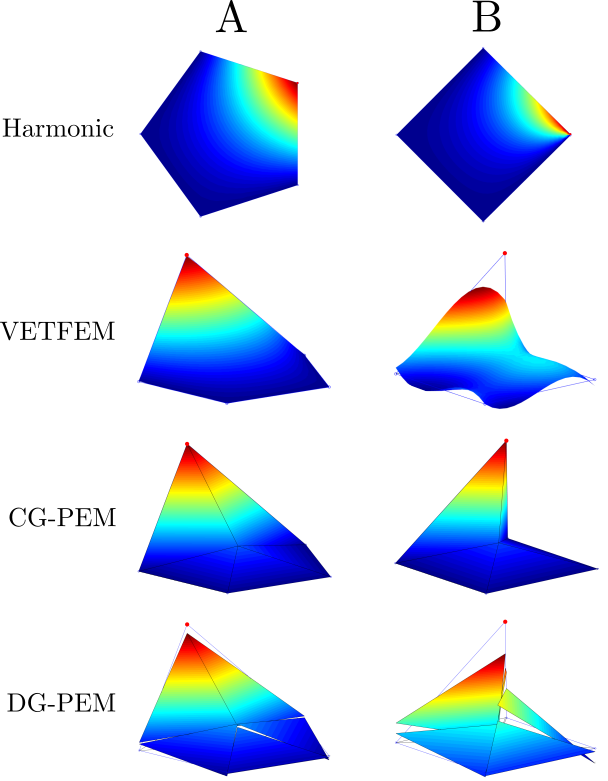
\includegraphics[width=5.0in]{figures/degenerate_element_comparison.pdf}  \caption{Comparison of shape functions computed for the two pentagonal elements with $l=1.0$ and $l=0.01$ using VETFEM, CG-PEM, and DG-PEM.}
  \label{fig:degenerate_element_comparison}
\end{figure}

As in the previous example, the aforementioned approximations were used in place of the harmonic shape functions when integrating the elements' elastic stiffness matrices. A comparison of the computed values for $\lambda_{\max}$ and $\lambda_{\min}$ is provided in table \ref{tab:degenerate_stiffness_max_min_eigenvalue}.

\begin{table}
\centering
\begin{subtable}{.5\textwidth}
\centering
\begin{tabular}{| c || c | c |}
    \hline
             & $l=1.0$ & $l=0.01$ \\ \hline \hline
    Harmonic & 0.9510 & 5.0899 \\ \hline
    VETFEM   & 0.9510 & 1.6818 \\ \hline
    CG-PEM   & 1.1326 & 64.098 \\ \hline
    DG-PEM   & 0.9510 & 1.3085 \\
    \hline
    \end{tabular}
    \caption{Largest eigenvalue: $\lambda_{\max}$}
    \label{tab:degenerate_stiffness_max_eigenvalue}
\end{subtable}% <---- don't forget this %
\begin{subtable}{.5\textwidth}
\centering
\begin{tabular}{| c || c | c |}
    \hline
             & $l=1.0$ & $l=0.01$ \\ \hline \hline
    Harmonic & 0.4925 & 0.3951 \\ \hline
    VETFEM   & 0.4906 & 0.3746 \\ \hline
    CG-PEM   & 0.8387 & 0.5516 \\ \hline
    DG-PEM   & 0.4739 & 0.2592 \\
    \hline
    \end{tabular}
    \caption{Smallest (non-zero) eigenvalue: $\lambda_{\min}$}
    \label{tab:degenerate_stiffness_min_eigenvalue}
\end{subtable}

\caption{Comparison of maximum and minimum (non-zero) eigenvalues of the element stiffness matrices computed for the elements shown in Figure \ref{fig:degenerate_element_shapes}.}
\label{tab:degenerate_stiffness_max_min_eigenvalue}
\end{table}

As noted in the previous example, the CG-PEM consistently over-estimates the eigenvalue spectra of the elements. Using a coarse (edge-based) partition further degrades the accuracy of the CG-PEM shape functions, to the extent that higher-order modes of deformation are severely over-stiff. Upon decreasing the edge length $l$ further, the maximum eigenvalue was observed to increase as $\lambda_{\max} \approx O (l^{-1})$. By comparison, the eigenvalue spectra for the VETFEM and DG-PEM remain small (well-conditioned), and relatively constant as $l \rightarrow 0$. The VETFEM, however, is observed to yield oscillatory solutions for the shape functions with decreasing $l$.

While the aforementioned insensitivity of the DG-PEM's eigenvalue spectra to short edges appears to be a desirable quality, it remains to be seen whether this is indeed the case. Correspondingly, the following series of investigations seeks to evaluate the implications of this property in a practical context.

\subsection*{Meshes Consisting of Elements with Degenerate Edges}

It is demonstrated herein that for certain element formulations, an over-abundance of short edges can potentially degrade the quality of the resulting finite element solution. Consider the two square patches depicted in Figure \ref{fig:polygonal_patches}, each containing 1,000 polygonal elements. Both meshes were generated using PolyMesher, a polygonal meshing tool detailed in \cite{Talischi:12}. The Voronoi mesh in Figure \ref{fig:patch_mesh} was obtained by a random point sampling process, and contains numerous elements with short edges. The mesh in Figure \ref{fig:lloyd_mesh} was obtained after 100 iterations of Lloyd's algorithm, yielding a polygonal mesh with reasonably well-proportioned elements. Additionally, any remaining short edges in the mesh of Figure \ref{fig:lloyd_mesh} were collapsed out according to the procedure described in \cite{Talischi:12}.
\begin{figure}[!h]
    \centering
    \begin{subfigure}[b]{0.49\linewidth}
            \centering
            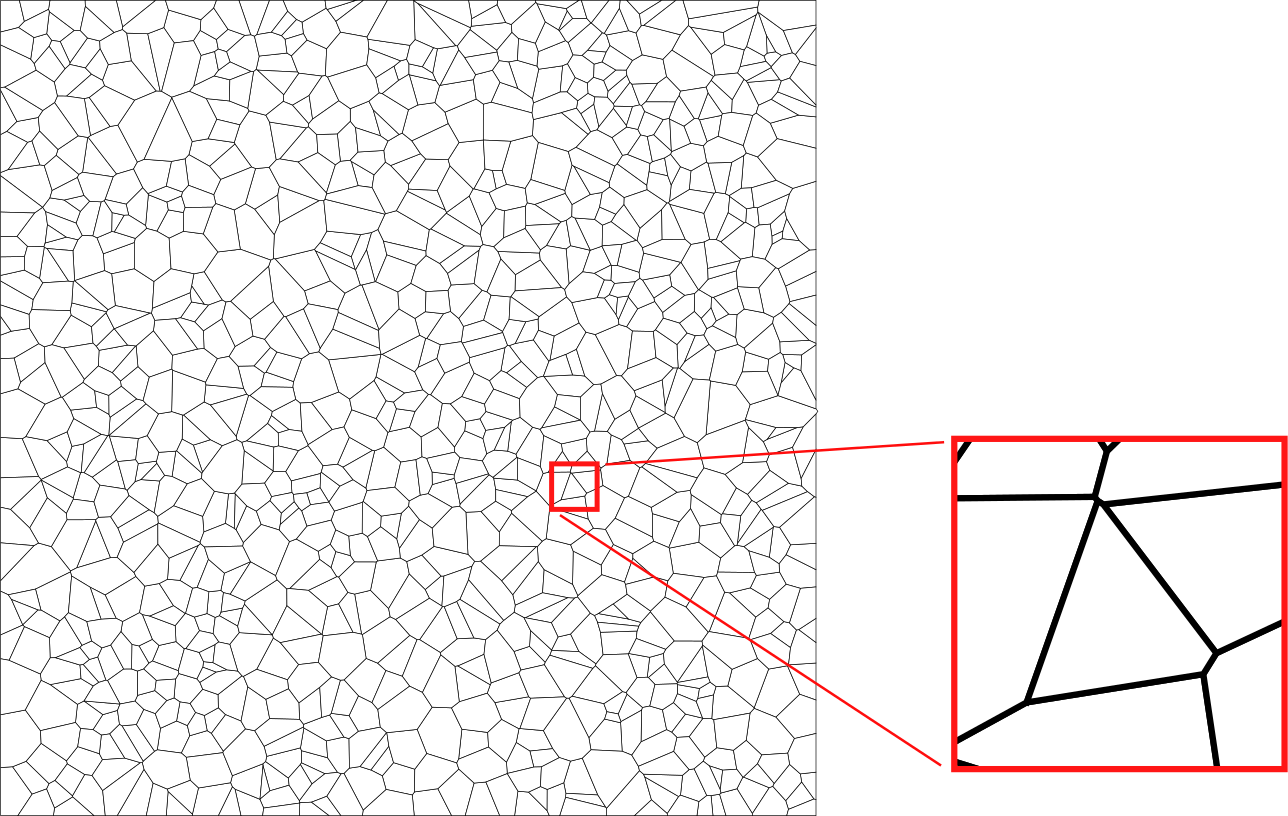
\includegraphics[width=3.0in]{figures/patch_mesh.pdf}
    			\caption{Random Voronoi mesh \label{fig:patch_mesh}}
    \end{subfigure}
	\begin{subfigure}[b]{0.49\linewidth}
            \centering
            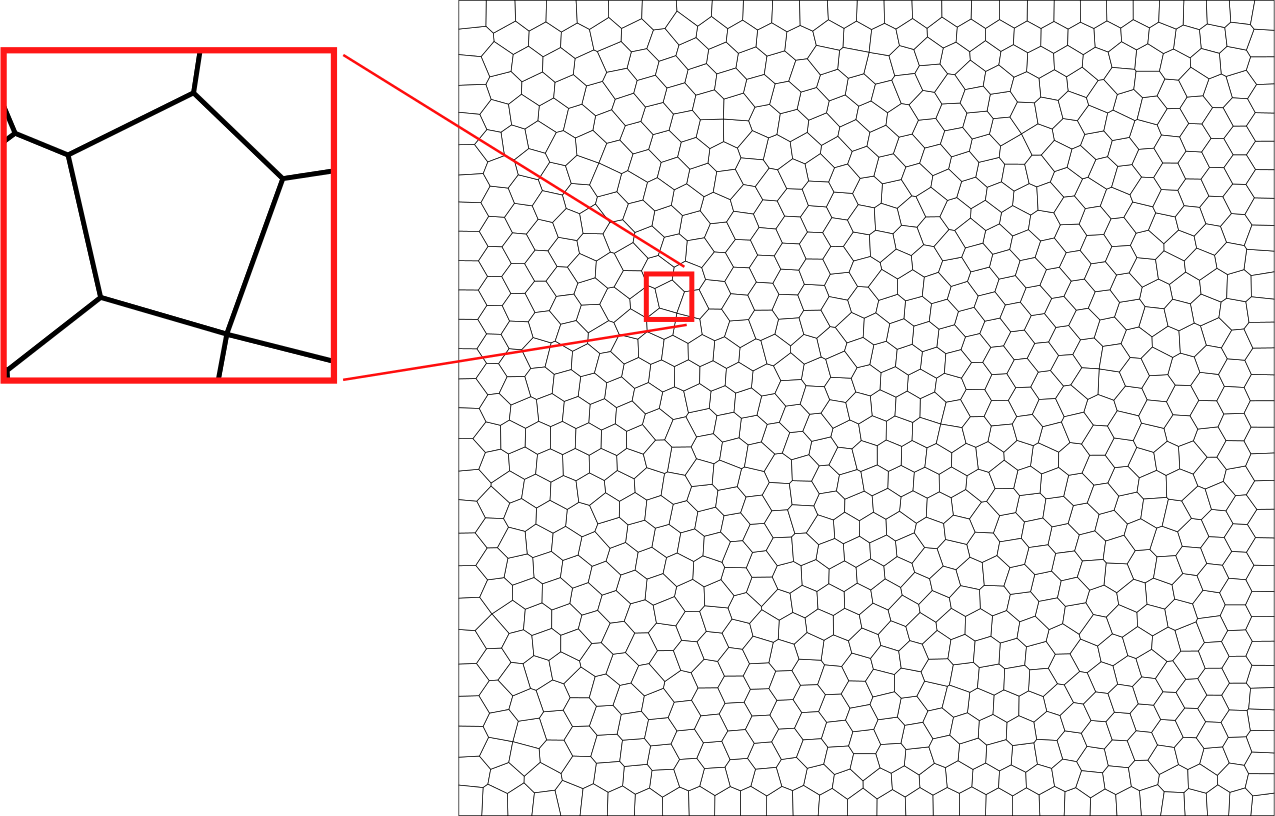
\includegraphics[width=3.0in]{figures/lloyd_mesh.pdf}
    			\caption{Lloyd mesh (100 iterations) \label{fig:lloyd_mesh}}
    \end{subfigure}
    \caption{Patches generated by PolyMesher, each containing 1,000 polygonal elements.}
    \label{fig:polygonal_patches}
\end{figure}

First, some preliminary definitions are provided for a number of relevant mesh metrics. For every polygonal element $\Omega_e \subset \mathbb{R}^2$, let $h_e$ denote the diameter of $\Omega_e$, such that
\begin{equation}
	h_e = \sup_{\mathbf{X}_1, \mathbf{X}_2 \in \Omega_e} || \mathbf{X}_1 - \mathbf{X}_2 ||_2.
\end{equation}
Further, denote by $|E|$ the length of any edge $E \subset \partial \Omega_e$, and define $\rho_e$ as the ratio of the smallest edge length $|E|$ divided by the element diameter $h_e$, i.e.
\begin{equation}
	\rho_e = \max_{E \subset \partial \Omega_e} \frac{|E|}{h_e}.
\end{equation}

For the meshes depicted in Figure \ref{fig:polygonal_patches}, the aforementioned edge length metrics were computed for all elements and edges in each mesh. Several histograms which characterize this data are provided in Figure \ref{fig:patch_edge_metrics}.
\begin{figure}[!h]
    \centering
    \begin{subfigure}[b]{0.49\linewidth}
            \centering
            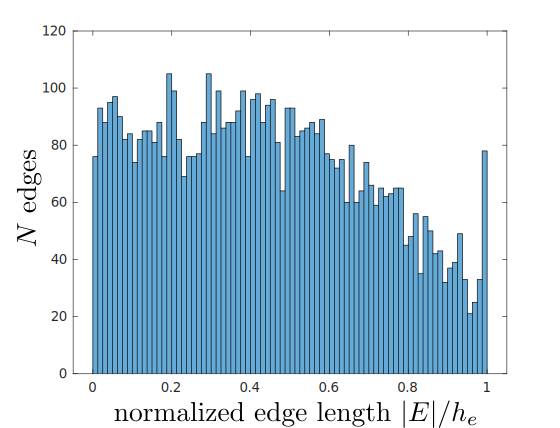
\includegraphics[width=3.0in]{figures/patch_edge_lengths.pdf}
    			\caption{Voronoi mesh \label{fig:patch_edge_lengths}}
    \end{subfigure}
	\begin{subfigure}[b]{0.49\linewidth}
            \centering
            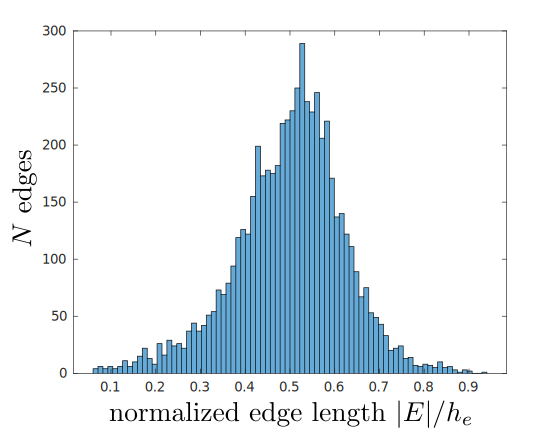
\includegraphics[width=3.0in]{figures/lloyd_edge_lengths.pdf}
    			\caption{Lloyd mesh \label{fig:lloyd_edge_lengths}}
    \end{subfigure}
    \begin{subfigure}[b]{0.49\linewidth}
            \centering
            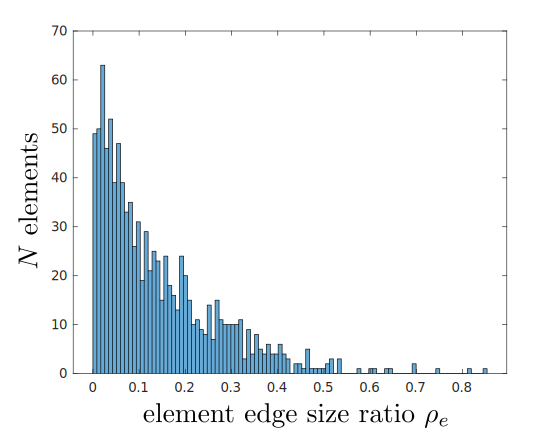
\includegraphics[width=3.0in]{figures/patch_edge_ratios.pdf}
    			\caption{Voronoi mesh \label{fig:patch_edge_ratios}}
    \end{subfigure}
	\begin{subfigure}[b]{0.49\linewidth}
            \centering
            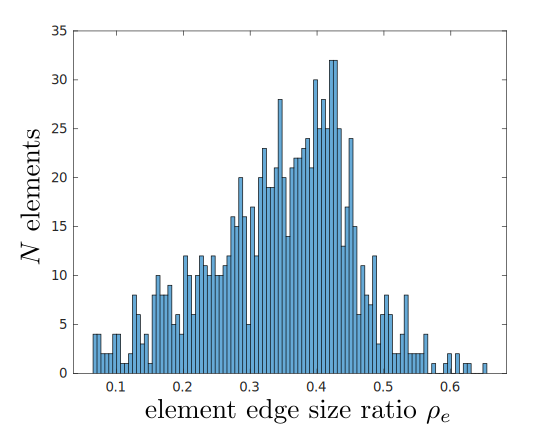
\includegraphics[width=3.0in]{figures/lloyd_edge_ratios.pdf}
    			\caption{Lloyd mesh \label{fig:lloyd_edge_ratios}}
    \end{subfigure}
    \caption{Histograms of various mesh metrics associated with the polygonal meshes depicted in Figure \ref{fig:polygonal_patches}:  (\subref{fig:patch_edge_lengths}) and (\subref{fig:lloyd_edge_lengths}) show the distributions of edge lengths contained in the random Voronoi and Lloyd meshes, respectively. (\subref{fig:patch_edge_ratios}) and (\subref{fig:lloyd_edge_ratios}) show the distributions for the smallest edge length ratios $\rho_e$ in the random Voronoi and Lloyd meshes, respectively.}
    \label{fig:patch_edge_metrics}
\end{figure}

A key observation regarding Figure \ref{fig:patch_edge_metrics} concerns the distribution of edge lengths within the random Voronoi mesh. The normalized lengths of all edges in the Voronoi mesh appear to be distributed almost uniformly, as seen in Figure \ref{fig:patch_edge_lengths}. Nonetheless, Figure \ref{fig:patch_edge_ratios} suggests that there is a relatively high probability that any given element in the random Voronoi mesh will contain at least one short edge. By comparison, the distributions for $|E|/h_e$ and $\rho_e$ in the Lloyd mesh are more Gaussian in nature, as demonstrated by Figures \ref{fig:lloyd_edge_lengths} and \ref{fig:lloyd_edge_ratios}, respectively.

To quantify the potential impact of short edges on finite element solution accuracy, the eigenvalue spectra of each patch's global stiffness matrix $\mathbf{K}$ were examined. Excessively large eigenvalues (particularly for the Voronoi mesh) may indicate solution sensitivity to the choice of discretization.

Each patch was specified to have unit dimensions ($1 \times 1$) and material properties ($E = 1.0$, $\nu = 0.0$). Global stiffness matrices were assembled for the two polygonal meshes shown in Figure \ref{fig:polygonal_patches} using the CG-PEM and the DG-PEM. Both formulations employed an edge-based partitioning scheme with composite mid-point quadrature on each element. The DG-PEM parameters were specified as $\epsilon = +1$, $\alpha_{\gamma0} = 10$, and $\alpha_{\gamma1} = 0$. The resulting eigenvalue spectra are plotted in Figure \ref{fig:patch_eigenvalue_distributions}.

\begin{figure}[!h]
  \centering
  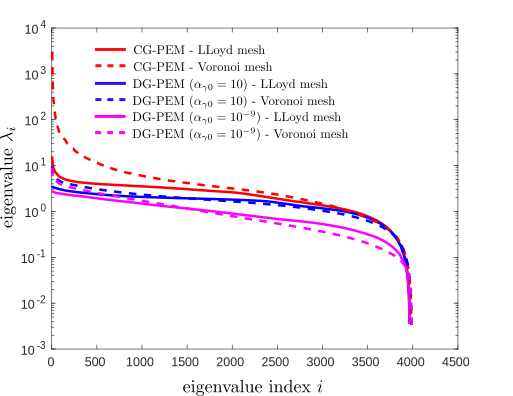
\includegraphics[width=5.0in]{figures/eigenvalue_distributions.pdf}  \caption{Eigenvalue spectra $\left\{ \lambda_i \right\}_{i = 1}^{N-3}$ for the (elastic) global stiffness matrix $\mathbf{K}$, computed for the CG-PEM and the DG-PEM ($\epsilon = +1$, $\alpha_{\gamma1} = 0$).}
  \label{fig:patch_eigenvalue_distributions}
\end{figure}

For the Lloyd mesh, both the CG-PEM and DG-PEM produce fairly comparable eigenvalue spectra. For the random Voronoi mesh, the CG-PEM produces higher-energy modes with significantly larger eigenvalues than the DG-PEM. Interestingly, the DG-PEM yields very similar eigenvalue spectra for both meshes. This appears to indicate a diminished sensitivity of the DG-PEM solution to the chosen discretization. Importantly, the behavior of the lower-energy modes remains the same across all meshes and element formulations. Figure \ref{fig:patch_eigenmodes_DGPEM} depicts the lowest-energy mode shapes determined by the DG-PEM. Similar mode shapes and corresponding eigenvalues were obtained for the CG-PEM.
\begin{figure}[!h]
  \centering
  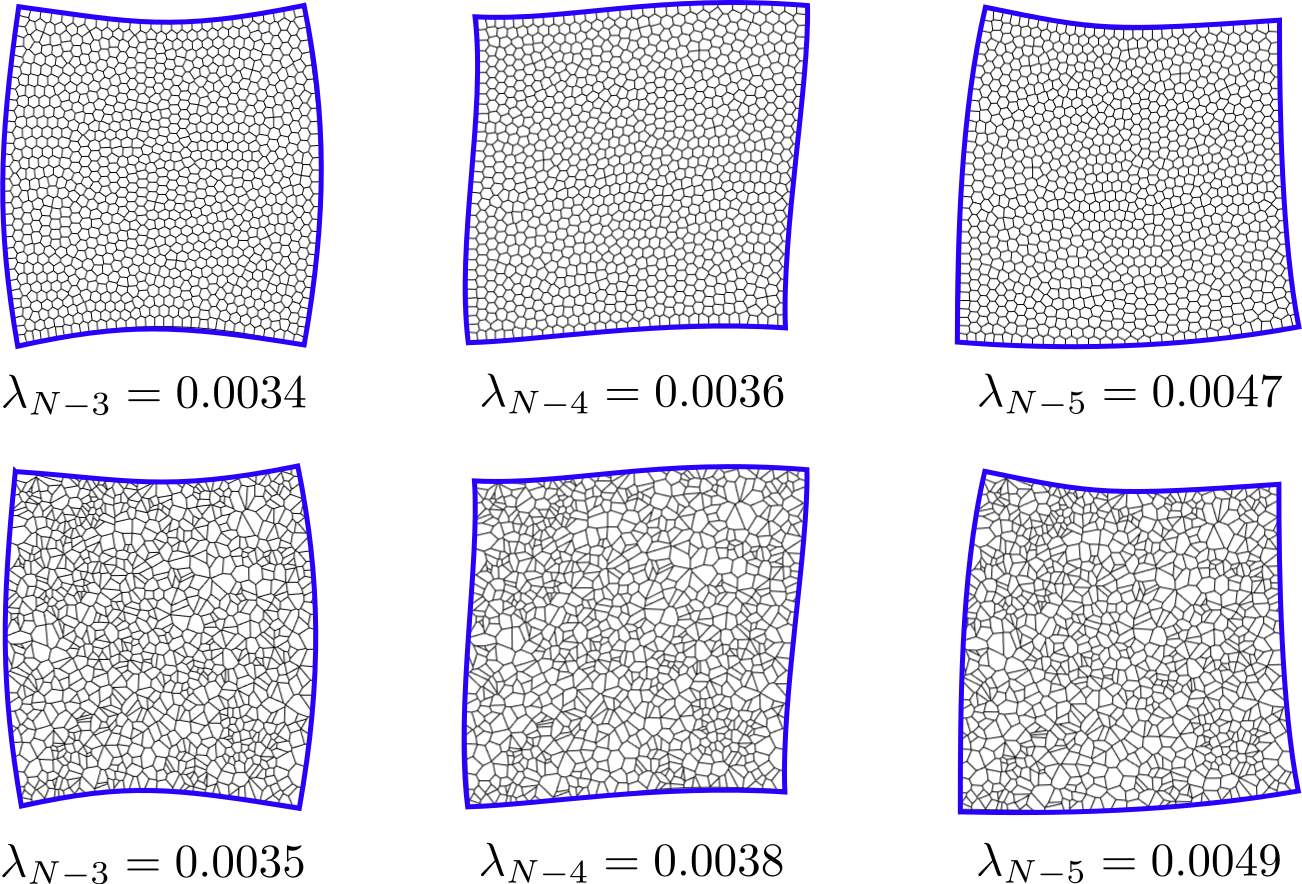
\includegraphics[width=5.0in]{figures/patch_eigenmodes_DGPEM.pdf}  \caption{Depiction of the smallest non-zero eigenvalues and corresponding eigenmodes computed using the DG-PEM ($\epsilon = +1$, $\alpha_{\gamma0} = 10$, $\alpha_{\gamma1} = 0$). $N$ denotes the size of the global stiffness matrix $\mathbf{K}$, and $\lambda_{N} = \lambda_{N-1} = \lambda_{N-2} = 0$ correspond to the zero-energy modes of deformation.}
  \label{fig:patch_eigenmodes_DGPEM}
\end{figure}

It is stressed that the results obtained for the DG-PEM will vary depending on the choice of penalty parameters $\alpha_{\gamma0}$ and $\alpha_{\gamma1}$. As $\alpha_{\gamma0} \rightarrow \infty$ the behavior of the CG-PEM is recovered. The corresponding variability in the condition number of $\mathbf{K}$ is characterized in Table \ref{tab:global_stiffness_condition_number}.
\begin{table}[!ht]
  \begin{center}
    \begin{tabular}{| c || c | c |}
    \hline
           & Voronoi mesh & Lloyd mesh \\ \hline \hline
    CG-PEM & 9.1e+05 & 4.6e+03 \\ \hline
    DG-PEM ($\alpha_{\gamma0} = 10^3$) & 4.8e+04 & 4.4e+03 \\ \hline
    DG-PEM ($\alpha_{\gamma0} = 10^1$) & 2.9e+03 & 1.0e+03 \\ \hline
    DG-PEM ($\alpha_{\gamma0} = 10^{-1}$) & 2.7e+03 & 8.1e+02  \\ \hline
    DG-PEM ($\alpha_{\gamma0} = 10^{-9}$) & 2.7e+03 & 8.1e+02 \\
    \hline
    \end{tabular}
    \caption{Computed values for the condition number $\kappa(\mathbf{K})$ of the global stiffness matrix $\mathbf{K}$ (excluding rigid body modes).}
    \vspace{-5pt}
    \label{tab:global_stiffness_condition_number}
    \vspace{-25pt}
  \end{center}
\end{table}

The condition number of the resulting global stiffness matrix will become large (asymptotically approaching that of the CG-PEM) as $\alpha_{\gamma0}$ is increased. Conversely, decreasing $\alpha_{\gamma0}$ lowers the condition number of $\mathbf{K}$, achieving an apparent lower-bound on $\kappa (\mathbf{K})$ in the limit as $\alpha_{\gamma0} \rightarrow 0$. Importantly, the resulting stiffness matrix does not contain spurious zero-energy modes, regardless of the choice of $\alpha_{\gamma0}$. Consequently, $\alpha_{\gamma0}$ should not be regarded as a type of hourglass control parameter, as any choice of $\alpha_{\gamma0} > 0$ will yield adequate stability.

% FEPEM - lloyd
% Max E = 1.6e+1
% Mix E = 3.5e-03
% E Rat = 4.6e+03

% FEPEM - patch
% Max E = 3.0e+03
% Mix E = 3.3e-03
% E Rat = 9.1e+05
% Min Emodes:  0.0034, 0.0036, 0.0047

% DGPEM - lloyd - A0 = 1.0e+3
% Max E = 1.5e+1
% Mix E = 3.5e-03
% E Rat = 4.4e+03
% Min Emodes: 0.0035, 0.0038, 0.0049

% DGPEM - patch - A0 = 1.0e+3
% Max E = 1.6e+02
% Mix E = 3.3e-03
% E Rat = 4.8e+04

% DGPEM - lloyd - A0 = 1.0e+1
% Max E = 3.6e+00
% Mix E = 3.5e-03
% E Rat = 1.0e+03

% DGPEM - patch - A0 = 1.0e+1
% Max E = 9.6e+00
% Mix E = 3.3e-03
% E Rat = 2.9e+03

% DGPEM - lloyd - A0 = 1.0e-1
% Max E = 2.8e+00
% Mix E = 3.5e-03
% E Rat = 8.1e+02

% DGPEM - patch - A0 = 1.0e-1
% Max E = 8.9e+00
% Mix E = 3.3e-03
% E Rat = 2.7e+03

%\begin{figure}[!h]
%    \centering
%    \begin{subfigure}[b]{0.49\linewidth}
%            \centering
%            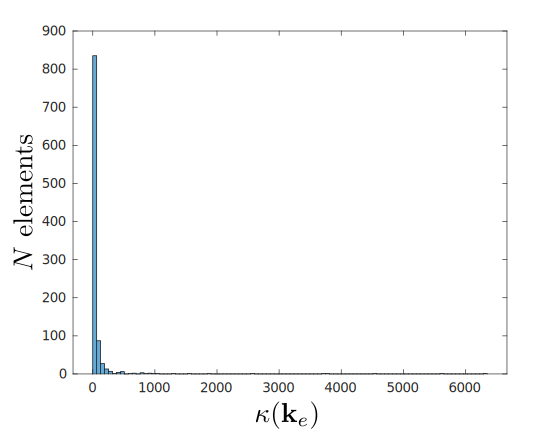
\includegraphics[width=3.0in]{figures/patch_condition_number_FEPEM.pdf}
%    			\caption{CG-PEM on the Voronoi mesh  \label{fig:patch_condition_number_FEPEM}}
%    \end{subfigure}
%	\begin{subfigure}[b]{0.49\linewidth}
%            \centering
%            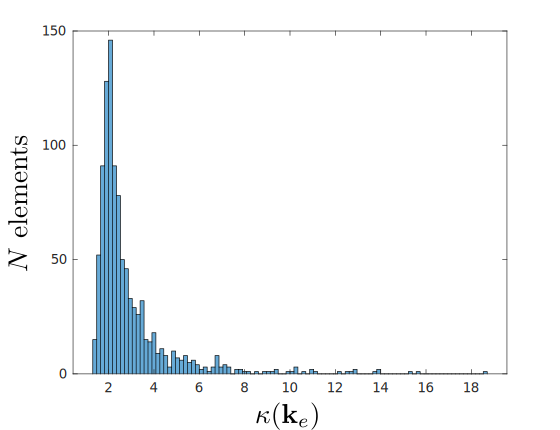
\includegraphics[width=3.0in]{figures/lloyd_condition_number_FEPEM.pdf}
%    			\caption{CG-PEM on the Lloyd mesh  \label{fig:lloyd_condition_number_FEPEM}}
%    \end{subfigure}
%    \begin{subfigure}[b]{0.49\linewidth}
%            \centering
%            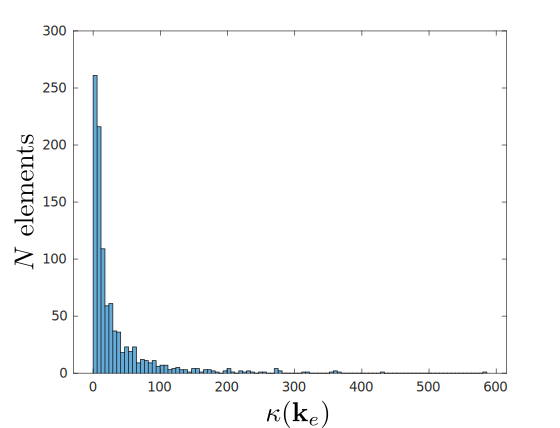
\includegraphics[width=3.0in]{figures/patch_condition_number_DGPEM.pdf}
%    			\caption{DG-PEM on the Voronoi mesh  \label{fig:patch_condition_number_DGPEM}}
%    \end{subfigure}
%	\begin{subfigure}[b]{0.49\linewidth}
%            \centering
%            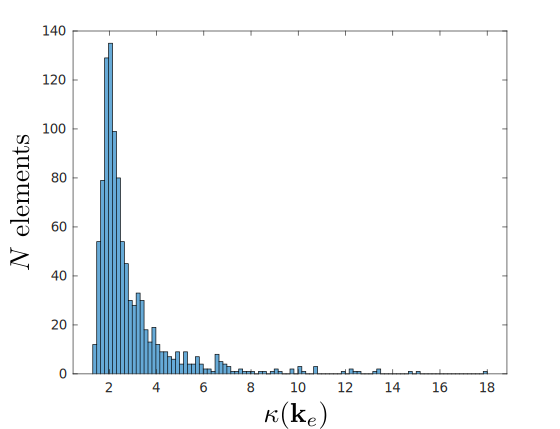
\includegraphics[width=3.0in]{figures/lloyd_condition_number_DGPEM.pdf}
%    			\caption{DG-PEM on the LLoyd mesh  \label{fig:lloyd_condition_number_DGPEM}}
%    \end{subfigure}
%    \caption{Histograms of various element metrics associated with the polygonal meshes depicted in Figure \ref{fig:polygonal_patches}:  (\subref{fig:patch_edge_lengths}) and (\subref{fig:lloyd_edge_lengths}) show the distributions of edge lengths contained in the random Voronoi and Lloyd meshes, respectively; (\subref{fig:patch_edge_ratios}) and (\subref{fig:lloyd_edge_ratios}) show the distributions for the smallest edge length ratios $\rho_e$ in the random Voronoi and Lloyd meshes, respectively.}
%\end{figure}

% local condition number investigation
	% look at DG-PEM system conditioning for certain degenerate elements
	%	* construct a random voronoi mesh on a 2d patch of elements
	%		- get edge-length metrics for voronoi cells
	%   		- examine condition number of local DGPEM systems on these elems
	%       - examine condition number of local stiffness matricies
	%			* look at max and min eigenvalues
	%		- check partition of unity and linear completeness passage
	%		- after grad correction, examine satisfaction of patch tests
	%	* do this for quadratic elements, as well
	%	* do parameter sensitivity analysis
	%	* look at global stiffness matrix condition number
	% look at conditioning for plate-like geometry (anisotropic patch tests)

% check via a series of single-element tests:
	% - examine a test involving a single non-convex element
	%   * shift node around, showing behavior vs. parameterized location
	%     - compare results for VETFEM, DGPEM, and FEPEM vs true harmonic SF
	%     - look at:
	%       * max and min eigenvalues of resulting stiffness matrix
	%       * comment on condition number, and effect on 
	%   * choose different partitioning algorithms / refinement levels
	%   * play around with DGPEM penalization parameters
	%   * examine effects of choosing DG
	% - do a test with a patch of non-convex elements
	%   * examine effects on global stiffness matrix conditioning
	%	* parameterized non-convexity, 

\section{Convergence Studies}

A series of studies were carried out to determine the convergence behavior of the DG-PEM. Several studies were conducted to verify that the DG-PEM yields a convergent sequences of approximations to a given problem under mesh refinement. A few relatively simple two- and three-dimensional elasticity problems are considered. Convergence results for the DG-PEM are compared against FEM, using both linear and quadratic elements in each case.

\subsection*{Infinite Elastic Plate in Far-Field Tension}

\begin{figure}[!h]
  \centering
  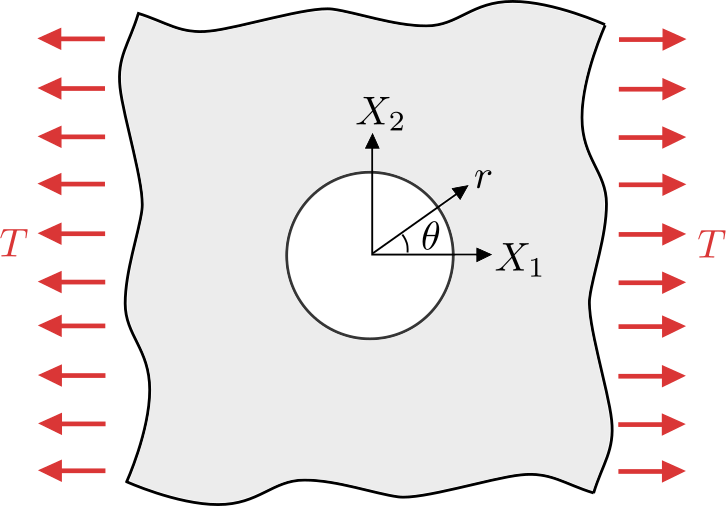
\includegraphics[width=4.0in]{figures/plate_with_hole.pdf}  \caption{Infinite plate with a circular hole placed in uniaxial tension.}
  \label{fig:plate_with_hole_problem}
\end{figure}
To demonstrate optimal convergence of the PEM for higher-order elements, we will choose to investigate the 2D elastostatics problem of an infinite plate with a circular hole in uniaxial tension (depicted in figure \ref{fig:plate_with_hole_problem}), for which there exist analytical solutions of the resulting displacement and stress fields (obtained from reference \cite{Wikiversity:17}):
\begin{equation}
  u_1 (r,\theta) = \frac{Ta}{8\mu} \left[ \frac{r}{a} (\kappa + 1) \cos \theta + \frac{2a}{r} ((1+\kappa) \cos \theta + \cos 3 \theta) - \frac{2a^3}{r^3} \cos 3 \theta \right]
\end{equation}
\begin{equation}
  u_2 (r,\theta) = \frac{Ta}{8\mu} \left[ \frac{r}{a} (\kappa - 3) \sin \theta + \frac{2a}{r} ((1-\kappa) \sin \theta + \sin 3 \theta) - \frac{2a^3}{r^3} \sin 3 \theta \right]
\end{equation}
\begin{equation}
  \sigma_{11} (r, \theta) = T - T \frac{a^2}{r^2} \bigg( \frac{3}{2} \cos 2 \theta + \cos 4 \theta \bigg) + T \frac{3a^4}{2r^4} \cos 4 \theta
\end{equation}
\begin{equation}
  \sigma_{22} (r, \theta) = - T \frac{a^2}{r^2} \bigg( \frac{1}{2} \cos 2 \theta - \cos 4 \theta \bigg) - T \frac{3a^4}{2r^4} \cos 4 \theta
\end{equation}
\begin{equation}
  \sigma_{12} (r, \theta) = - T \frac{a^2}{r^2} \bigg( \frac{1}{2} \sin 2 \theta + \sin 4 \theta \bigg) + T \frac{3a^4}{2r^4} \sin 4 \theta
\end{equation}
where $T$ is the far-field value of the applied tensile stress, $a$ is the radius of the circular hole centered at $r=0$, $\kappa = 4 - 3\nu$ (under plane-strain conditions), and $\nu$ and $\mu$ are the the Poisson's ratio and shear modulus of the material, respectively.

\begin{figure}[!h]
  \centering
  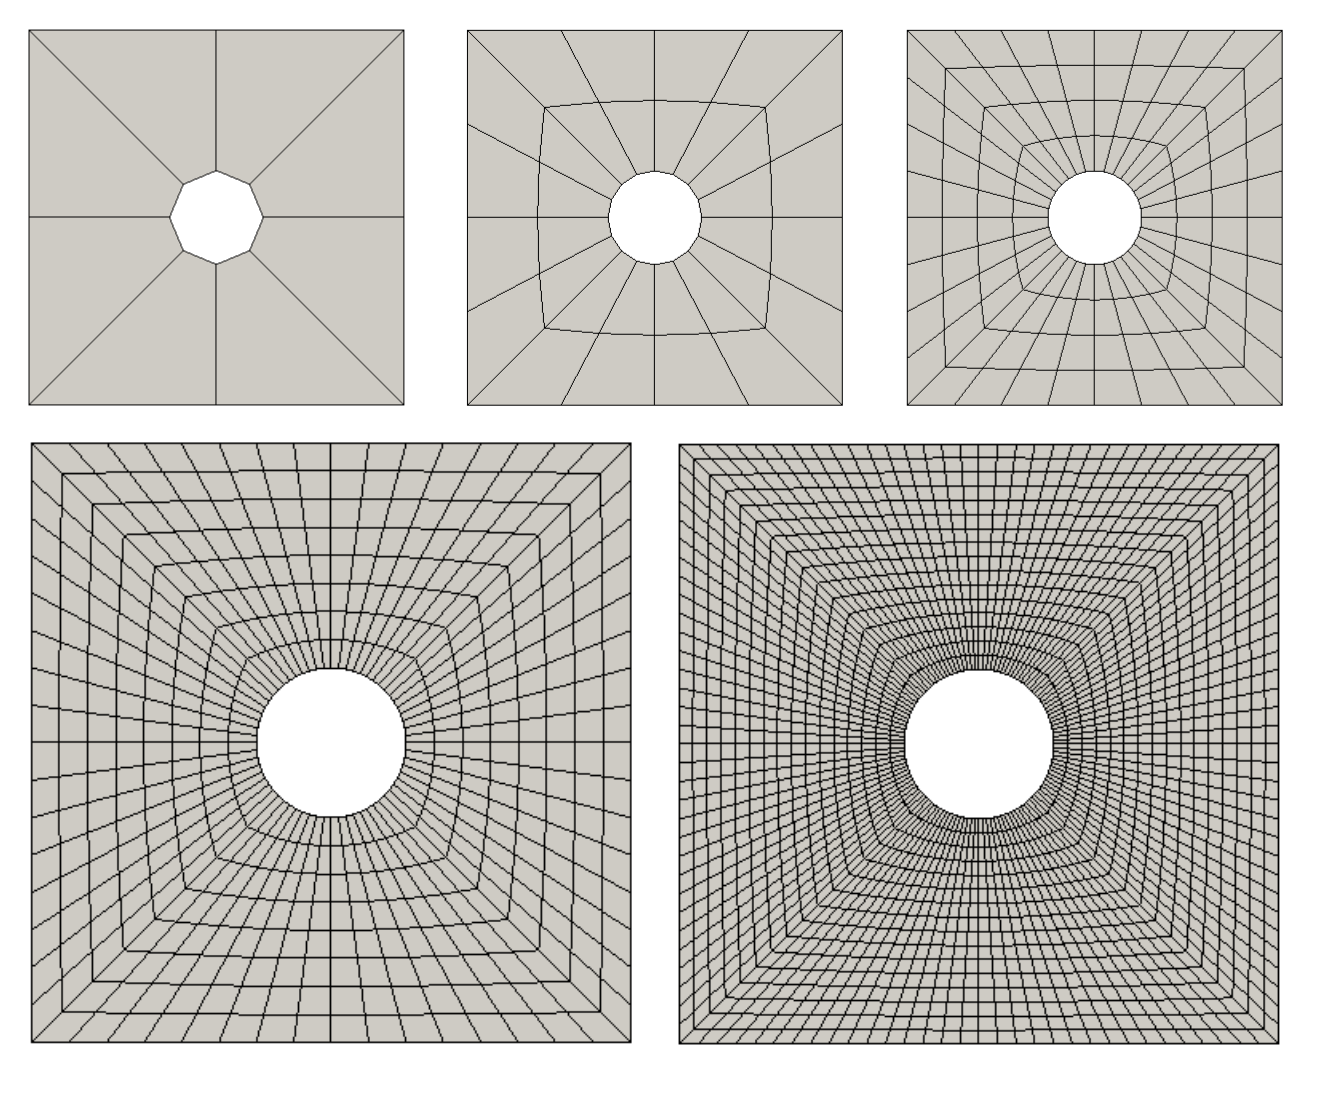
\includegraphics[width=6.0in]{figures/plate_with_hole_meshes.pdf}
  \caption{Quadrilateral meshes with varying levels of refinement.}
  \label{fig:plate_with_hole_meshes}
\end{figure}

A convergence study was carried out using a series of quadrilateral meshes with varying levels of refinement, discretizing the restricted problem domain $X_i \in [ -1, +1]$ (see figure \ref{fig:plate_with_hole_meshes}.) The meshes consisted of either 4-node quadrilateral or 8-node serendipity quadrilateral elements, and employed either an isoparametric formulation, or a sufficiently high-order DG-PEM formulation (i.e. $k=1$ for 4-node quadrilaterals, and $k=2$ for 8-node quadrilaterals.) Displacement boundary conditions were prescribed to be consistent with the exact solution on the restricted boundary. Displacement and stress error norms were computed with reference to the exact solution. Convergence plots for the displacement and stress error norms are provided in Figures \ref{fig:plate_with_hole_l2_errors} and \ref{fig:plate_with_hole_h1_errors}, respectively.

\begin{figure}[!h]
  \centering
    \begin{subfigure}[b]{0.49\linewidth}
            \centering
            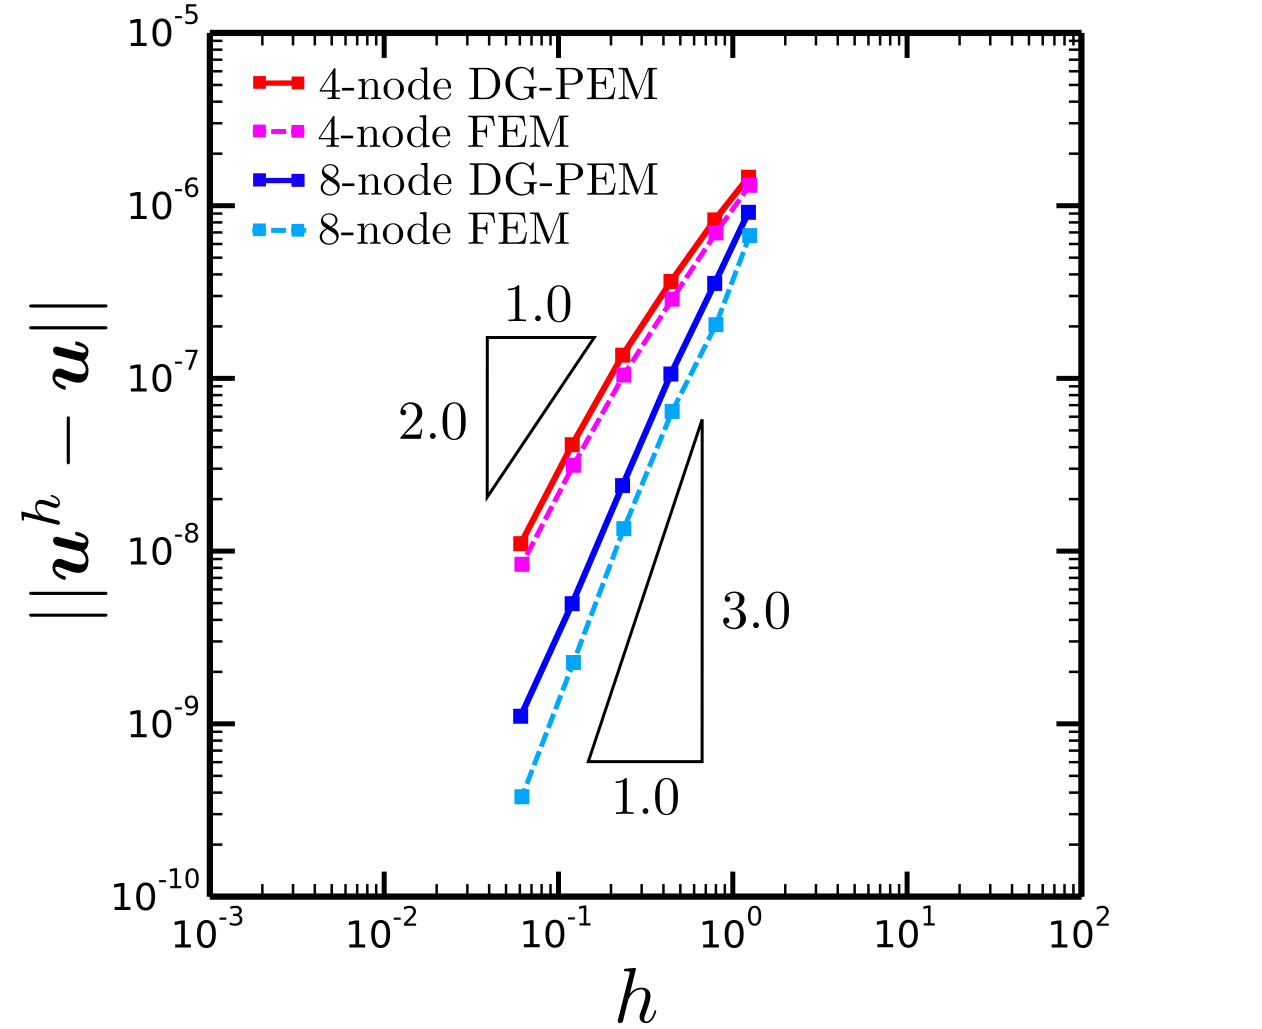
\includegraphics[width=3.3in]{figures/plate_with_hole_l2_errors.pdf}
    			\caption{displacement errors \label{fig:plate_with_hole_l2_errors}}
    \end{subfigure}
	\begin{subfigure}[b]{0.49\linewidth}
            \centering
            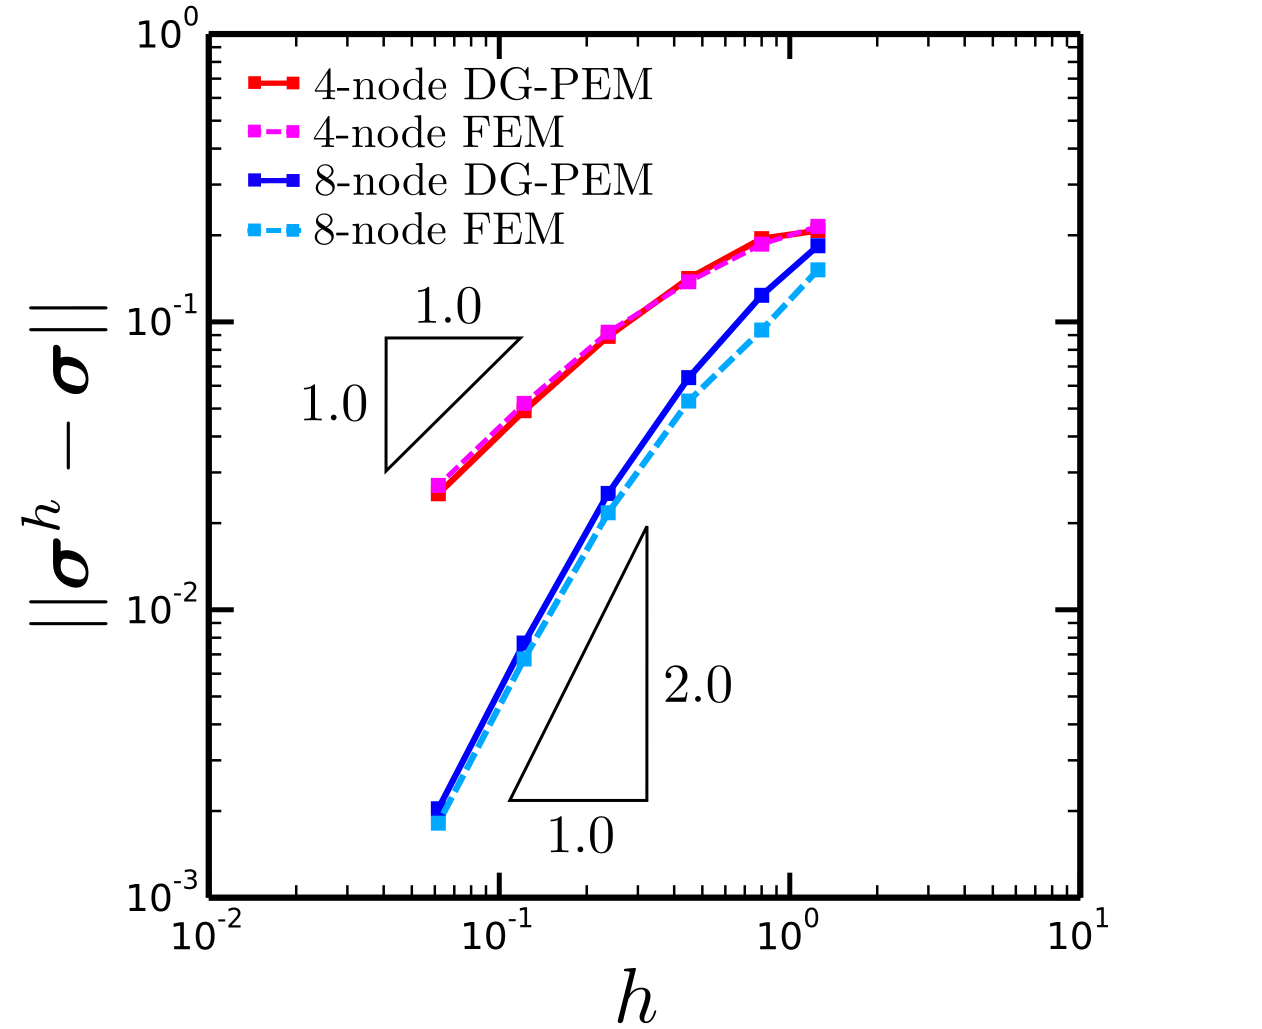
\includegraphics[width=3.3in]{figures/plate_with_hole_h1_errors.pdf}
    			\caption{stress errors \label{fig:plate_with_hole_h1_errors}}
    \end{subfigure} \caption{Convergence plots for the plate with hole problem using FEM and DG-PEM.}
  \label{fig:plate_with_hole_errors}
\end{figure}

For a given element formulation, the \textit{rate} of convergence in the two error metrics $|| \mathbf{u}^h - \mathbf{u} || \leq C h^p || \mathbf{u} ||$ and $|| \boldsymbol{\sigma}^h - \boldsymbol{\sigma} || \leq C h^q || \boldsymbol{\sigma} ||$ will be characterized by the powers $p$ and $q$, respectively. The average and maximal rates of convergence for each element formulation across all levels of mesh refinement are displayed in Table \ref{tab:plate_with_hole_convergence_rates}.

\begin{table}[!ht]
  \begin{center}
    \begin{tabular}{| c || c | c || c | c |}
    \hline
           & $p_{\text{avg}}$ & $p_{\text{max}}$ & $q_{\text{avg}}$ & $q_{\text{max}}$ \\ \hline \hline
    FEM (4-node quadrilateral)    & 1.66 (2.0) & 1.94 (2.0) & 0.66 (1.0) & 0.96 (1.0) \\ \hline
    DG-PEM (4-node quadrilateral) & 1.88 (2.0) & 2.13 (2.0) & 0.73 (1.0) & 0.99 (1.0) \\ \hline
    FEM (8-node quadrilateral)    & 2.48 (3.0) & 2.68 (3.0) & 1.43 (2.0) & 1.93 (2.0) \\ \hline
    DG-PEM (8-node quadrilateral) & 2.34 (3.0) & 3.02 (3.0) & 1.71 (2.0) & 2.42 (2.0) \\
    \hline
    \end{tabular}
    \caption{Average and maximal convergence rates $p_{\text{avg}}$ and $q_{\text{avg}}$ for each method. The optimal rates are shown in parentheses.}
    \vspace{-5pt}
    \label{tab:plate_with_hole_convergence_rates}
    \vspace{-25pt}
  \end{center}
\end{table}

It should be noted that part of the solution error incurred for the coarse meshes may be attributable to the inexact representation of the problem domain (the circular hole). This would explain why the observed convergence rates are lower at coarser levels of refinement, but approach the optimal rates as the mesh is further refined.

In the limit as $h \rightarrow 0$, the DG-PEM quadrilateral elements converge at the optimal rates in both the displacement and stress error norms. Because the quadrilateral meshes in Figure \ref{fig:plate_with_hole_meshes} consist of non-affinely distorted elements, the FEM using isoparametric serendipity elements does not achieve the optimal rates of convergence. Overall, the DG-PEM appears to converge at slightly faster rates than the FEM. However, the solution errors at coarser levels of refinement tends to be better for the FEM, in general.

Further work will seek to investigate the measured error and convergence rates of the PEM when the elements take on arbitrary shape, and for a variety of different formulations and penalization parameter settings.

\section{Sensitivity to Locking Phenomena}

\subsection*{Twisting Annulus}

Consider an incompressible elastic annulus whose inner radius at $r = R_i$ is fixed, and whose outer radius $r = R_o$ rigidly rotates at an angular velocity of $\Phi$. The radially symmetric displacement boundary conditions for this motion are described by
\begin{equation}
	u_r (R_i,t) = u_r (R_o,t) = 0, \quad u_z (R_i,t) = u_z (R_o,t) = 0,
\end{equation}
\begin{equation}
	u_\theta (R_i,t) = 0, \quad u_\theta (R_o,t) = R_o \, \Phi \, t,
\end{equation}
for all $t \geq 0$.

The elastic material is characterized by a linear hypoelastic material model of grade zero, obeying
\begin{equation}
  \dot{\boldsymbol{\sigma}} = \mathbb{C} : \mathbf{D} + \mathbf{W} \boldsymbol{\sigma} - \boldsymbol{\sigma} \mathbf{W},
\end{equation}

\subsubsection*{Exact Solution}

An exact solution for the aforementioned problem may be obtained by considering the stress divergence equations in cylindrical polar coordinates:
\begin{equation}
  \nabla \cdot \boldsymbol{\sigma} = \left\{ \begin{array}{c} \frac{\partial \sigma_{rr}}{\partial r} + \frac{\sigma_{rr}}{r} + \frac{1}{r} \frac{\partial \sigma_{\theta r}}{\partial \theta} + \frac{\partial \sigma_{z r}}{\partial z} - \frac{\sigma_{\theta \theta}}{r} \\
    \frac{1}{r} \frac{\partial \sigma_{\theta \theta}}{\partial \theta} + \frac{\partial \sigma_{r\theta}}{\partial r} + \frac{\sigma_{r\theta}}{r} + \frac{\sigma_{\theta r}}{r} + \frac{\partial \sigma_{z \theta}}{\partial z} \\
    \frac{\partial \sigma_{z z}}{\partial z} + \frac{\partial \sigma_{r z}}{\partial r} + \frac{\sigma_{r z}}{r} + \frac{1}{r} \frac{\partial \sigma_{\theta z}}{\partial \theta} \end{array} \right\} = \mathbf{0}.
\end{equation}
By the assumptions of plane strain and axisymmetry, we rationalize that $\boldsymbol{\sigma} (r)$ is a function of $r$, alone, and therefore,
\begin{equation}
  \nabla \cdot \boldsymbol{\sigma} = \left\{ \begin{array}{c} \frac{\partial \sigma_{rr}}{\partial r} + \frac{\sigma_{rr} - \sigma_{\theta \theta}}{r} \\
    \frac{\partial \sigma_{r\theta}}{\partial r} + \frac{2 \sigma_{r\theta}}{r} \\
    \frac{\partial \sigma_{r z}}{\partial r} + \frac{\sigma_{r z}}{r} \end{array} \right\} = \mathbf{0}.
\end{equation}
Furthermore, by the assumptions of plane strain, we observe that $\sigma_{rz} = 0$ and $\sigma_{\theta z} = 0$. Additionally, if we impose the incompressibility condition $\nabla \cdot \mathbf{v} = \text{tr} (\mathbf{D}) = 0$, we find that
\begin{equation}
  \text{tr} (\dot{\boldsymbol{\sigma}}) = 0 \, \Rightarrow \, \text{tr} (\boldsymbol{\sigma}) = 0 \, \forall t.
\end{equation}
The deformation necessitates that $\sigma_{zz} = 0$, and therefore $\sigma_{\theta \theta} = - \sigma_{rr}$. Consequently, we are left with 2 governing differential equations for $\sigma_{rr}$ and $\sigma_{r \theta}$:
\begin{equation}
  \frac{\partial \sigma_{rr}}{\partial r} + \frac{2 \sigma_{rr}}{r} = 0, \quad \frac{\partial \sigma_{r\theta}}{\partial r} + \frac{2 \sigma_{r\theta}}{r} = 0,
\end{equation}
whose solutions are of the form
\begin{equation}
  \sigma_{rr} = \frac{a}{r^2}, \quad \sigma_{r\theta} = \frac{b}{r^2}.
\end{equation}
Consequently,
\begin{equation}
  \left\{ \begin{array}{c} \sigma_{rr} \\ \sigma_{\theta \theta} \\ \sigma_{r \theta} \end{array} \right\} = r^{-2} \left\{ \begin{array}{c} +a \\ -a \\ b \end{array} \right\}.
\end{equation}

Under the assumption of incompressibility, we may characterize the deformation via the velocity field $v_r = 0$, $v_z = 0$, and $v_\theta (r) = r \dot{\phi}(r)$, yielding the velocity gradient (in cylindrical polar coordinates):
\begin{equation}
  \mathbf{L} = \nabla \mathbf{v} = \left[ \begin{array}{ccc} v_{r,r} & v_{r,\theta}/r-v_\theta /r & v_{r,z} \\
      v_{\theta,r} & v_{\theta,\theta}/r + v_r /r & v_{\theta,z} \\
      v_{z,r} & v_{z,\theta} /r & v_{z,z} \end{array} \right] = 
  \left[ \begin{array}{ccc} 0 & -\dot{\phi} & 0 \\
      \dot{\phi} + r \dot{\phi}_{,r} & 0 & 0 \\
      0 & 0 & 0 \end{array} \right],
\end{equation}
and the corresponding rate of deformation and spin tensors:
\begin{equation}
  \mathbf{D} = \frac{r \dot{\phi}_{,r}}{2} \left[ \begin{array}{ccc} 0 & 1 & 0 \\
      1 & 0 & 0 \\
      0 & 0 & 0 \end{array} \right], \quad \mathbf{W} = 
  \frac{2 \dot{\phi} + r \dot{\phi}_{,r}}{2} \left[ \begin{array}{ccc} 0 & - 1 & 0 \\
      1 & 0 & 0 \\
      0 & 0 & 0 \end{array} \right].
\end{equation}
The resulting stress rate equations are
\begin{equation}
  \left\{ \begin{array}{c} \dot{\sigma}_{rr} \\ \dot{\sigma}_{\theta \theta} \\ \dot{\sigma}_{r \theta} \end{array} \right\} = \left\{ \begin{array}{c} 0 \\ 0 \\ \mu r \dot{\phi}_{,r} \end{array} \right\} + 
  (2 \dot{\phi} + r \dot{\phi}_{,r}) \left\{ \begin{array}{c} - \sigma_{r \theta} \\ \sigma_{r \theta} \\ \sigma_{rr} \end{array} \right\},
\end{equation}
or
\begin{equation}
  \left\{ \begin{array}{c} \dot{a} \\ \dot{b} \end{array} \right\} = \left\{ \begin{array}{c} 0 \\ \mu r^3 \dot{\phi}_{,r} \end{array} \right\} + (2 \dot{\phi} + r \dot{\phi}_{,r}) \left[ \begin{array}{cc} 0 & -1 \\ 1 & 0 \end{array} \right] \left\{ \begin{array}{c} a \\ b \end{array} \right\},
\end{equation}
which must be valid $\forall r, \, t$. If we assume that $\dot{\phi} = f(r)$ is a function of $r$ (and not of $t$), then we obtain the condition
\begin{equation}
  3 f_{,r} + r f_{,rr} = 0,
\end{equation}
implying $f_{,r} = B r^{-3}$, and $\phi (r, t) = (A - B r^{-2} / 2)t$, thus
\begin{equation}
  \left\{ \begin{array}{c} \dot{a} \\ \dot{b} \end{array} \right\} = \left\{ \begin{array}{c} 0 \\ \mu B \end{array} \right\} + 2 A \left[ \begin{array}{cc} 0 & -1 \\ 1 & 0 \end{array} \right] \left\{ \begin{array}{c} a \\ b \end{array} \right\},
\end{equation}
and
\begin{equation}
  a(t) = - \frac{\mu B}{2 A} - C_2 \sin (2 A t) + C_1 \cos (2 A t),
\end{equation}
\begin{equation}
  b(t) = C_1 \sin (2 A t) + C_2 \cos (2 A t).
\end{equation}
Imposing the initial conditions $a(0) = b(0) = 0$ results in:
\begin{equation}
  a(t) = \frac{\mu B}{2 A} \left[ \cos (2 A t) - 1 \right], \quad b(t) = \frac{\mu B}{2 A} \sin (2 A t).
\end{equation}
Imposing the boundary conditions $\phi(R_i,t) = 0 \, \, \forall t$, $\phi(R_o,t) = \Phi \, t \, \, \forall t$ yields:
\begin{equation}
  A = \frac{\Phi R_i^{-2}}{R_i^{-2} - R_o^{-2}}, \quad B = \frac{2 \Phi}{R_i^{-2} - R_o^{-2}}.
\end{equation}

The final analytical solution for the displacement and stress fields is presented below:
\begin{equation}
  u_r = 0, \quad u_\theta = r \Phi \frac{R_i^{-2} - r^{-2}}{R_i^{-2} - R_o^{-2}} t, \quad u_z = 0,
\end{equation}
\begin{equation}
  \sigma_{rr} = - \sigma_{\theta \theta} = \mu \frac{r^{-2}}{R_i^{-2}} \left[ \cos \left( 2 \frac{\Phi R_i^{-2}}{R_i^{-2} - R_o^{-2}} t \right) - 1 \right],
\end{equation}
\begin{equation}
  \sigma_{r \theta} = \mu \frac{r^{-2}}{R_i^{-2}} \sin \left( 2 \frac{\Phi R_i^{-2}}{R_i^{-2} - R_o^{-2}} t \right).
\end{equation}

\subsubsection*{Numerical Results}

Because the element formulations that will be used herein possess only displacement degrees of freedom, we expect the finite element solutions to present inaccuracies due to the effects of volumetric locking. Moreover, it is not possible to run an analysis for a truly incompressible material (if the grade zero hypoelasticity model is to be utilized). For these reasons, it will suffice to examine solutions in the near-incompressible regime (i.e. $\nu = 0.4999$).

Additionally, because an accurate prediction of the pressure field requires the use of a mixed formulation, we expect that the stress error metric in (\ref{eq:normalized_stress_error}) will be dominated by errors in the pressure field. For this reason, we will choose to examine only the errors in the deviatoric stress:
\begin{equation}
	\frac{||\mathbf{s}^h - \mathbf{s}||}{||\mathbf{s}||} = \sqrt{\frac{\int_{\mathcal{B}_0} (\mathbf{s}^h - \mathbf{s}) \colon (\mathbf{s}^h - \mathbf{s}) \, dV}{\int_{\mathcal{B}_0} \mathbf{s} \colon \mathbf{s} \, dV}},
	\label{eq:normalized_stress_error}
\end{equation}
where $s_{ij} = \sigma_{ij} - \frac{1}{3} \delta_{ij} \sigma_{kk}$ denotes the stress deviator.

\begin{figure}[!h]
  \centering
  \includegraphics[width=6.0in]{figures/annulus_meshes.pdf}
  \caption{Polygonal meshes with varying levels of refinement for the twisting annulus problem.}
  \label{fig:annulus_meshes}
\end{figure}

\begin{figure}[!h]
  \centering
  \includegraphics[width=6.0in]{figures/quad_annulus_meshes.pdf}
  \caption{Quadrilateral meshes with varying levels of refinement for the twisting annulus problem.}
  \label{fig:quad_annulus_meshes}
\end{figure}

\begin{figure}[!h]
  \centering
    \begin{subfigure}[b]{0.49\linewidth}
            \centering
            \includegraphics[width=3.3in]{figures/quad_l2_error.pdf}
    			\caption{displacement error \label{fig:quad_l2_error}}
    \end{subfigure}
	\begin{subfigure}[b]{0.49\linewidth}
            \centering
            \includegraphics[width=3.3in]{figures/quad_h1_error.pdf}
    			\caption{stress deviator error \label{fig:quad_h1_error}}
    \end{subfigure} \caption{Convergence plots for the twisting annulus problem using standard isoparametric elements.}
  \label{fig:quad_error}
\end{figure}

\begin{figure}[!h]
  \centering
    \begin{subfigure}[b]{0.49\linewidth}
            \centering
            \includegraphics[width=3.3in]{figures/quad_l2_error.pdf}
    			\caption{displacement error \label{fig:quad_l2_error}}
    \end{subfigure}
	\begin{subfigure}[b]{0.49\linewidth}
            \centering
            \includegraphics[width=3.3in]{figures/quad_h1_error.pdf}
    			\caption{stress deviator error \label{fig:quad_h1_error}}
    \end{subfigure} \caption{Convergence plots for the twisting annulus problem using standard isoparametric elements.}
  \label{fig:quad_error}
\end{figure}

\subsection*{Thin Corner-Supported Plate}

Consider a thin plate 
(Description of the corner-supported plate problem).

\begin{figure}[!h]
  \centering
  \includegraphics[width=6.0in]{figures/plate_meshes.pdf}
  \caption{Hexahedral meshes with variable plate thickness $h$ and mesh perturbations $p$ for the corner-supported plate problem.}
  \label{fig:plate_meshes}
\end{figure}

\subsubsection{Exact Solution}

An exact solution for the vertical displacement field of the plate prob

\section{Computational Efficiency}

\subsection{Performance Comparison}



\section{Nonlinear Kinematics and Elastoplastic Material Behavior}

\subsection*{Ductile Necking Problem}

The $J_2$ model of elastoplasticity with linear isotropic hardening was implemented, employing the radial return algorithm described in \cite{LSDYNA}.

\begin{figure}[!h]
    \centering
    \begin{subfigure}[b]{0.49\linewidth}
            \centering
            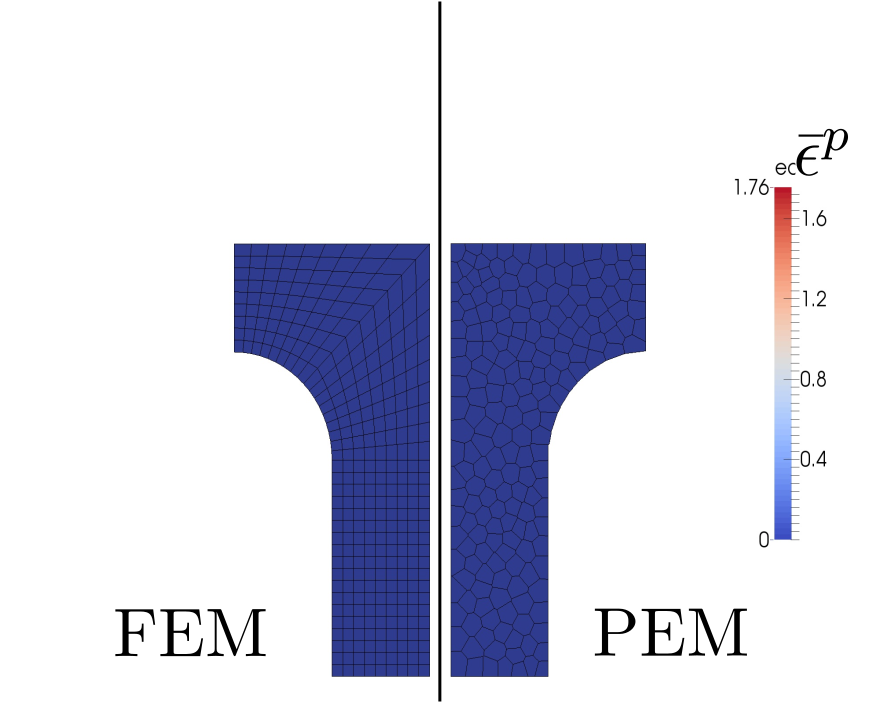
\includegraphics[width=3.0in]{figures/necking_eqps_0.pdf}
    			\caption{$t=0.0$ \label{fig:necking_eqps_0}}
    \end{subfigure}
	\begin{subfigure}[b]{0.49\linewidth}
            \centering
            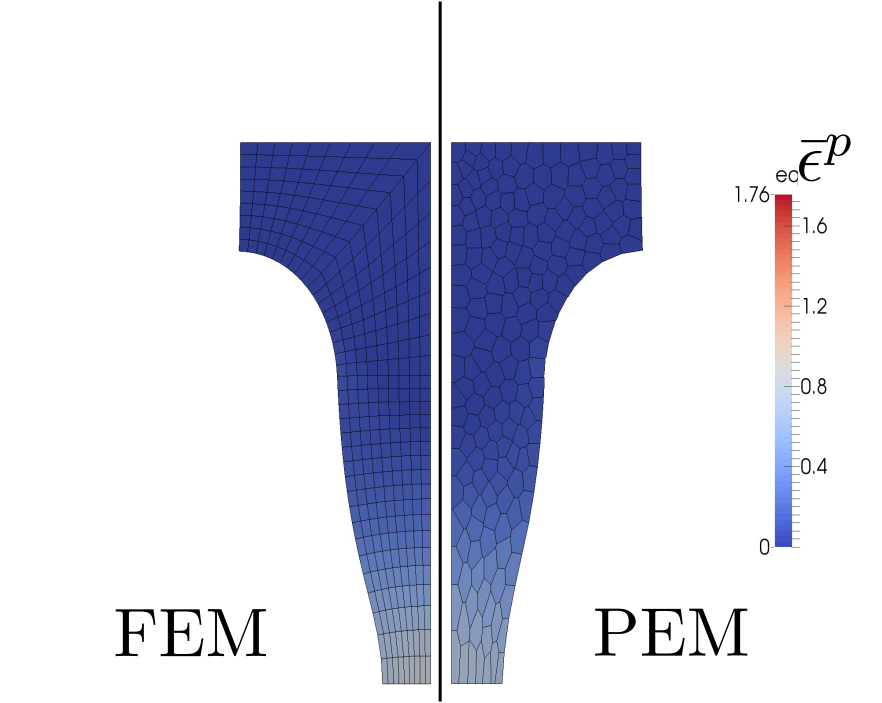
\includegraphics[width=3.0in]{figures/necking_eqps_1.pdf}
    			\caption{$t=0.5$ \label{fig:necking_eqps_1}}
    \end{subfigure}
    \begin{subfigure}[b]{0.49\linewidth}
            \centering
            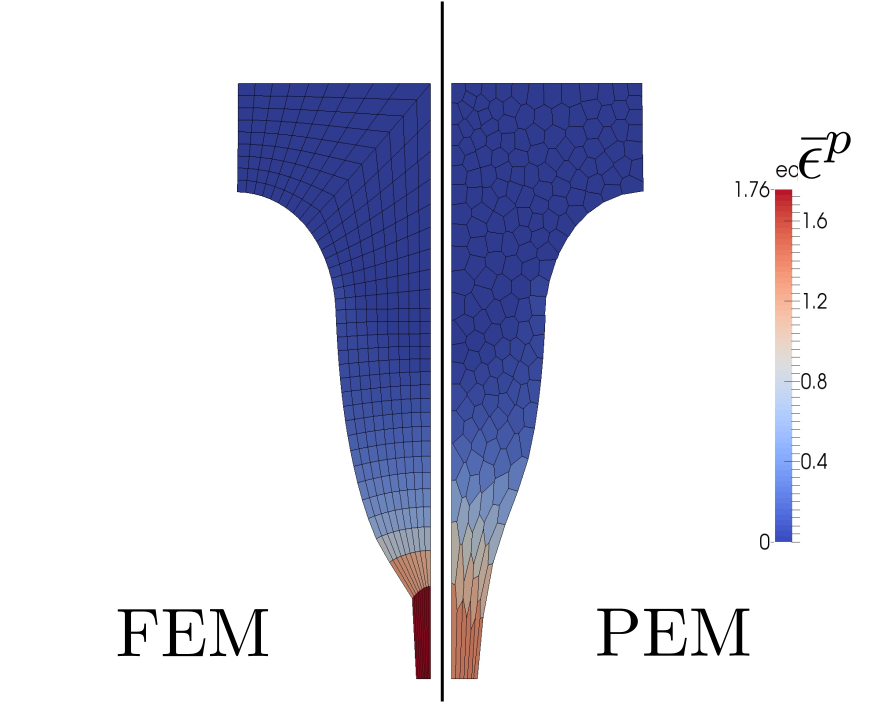
\includegraphics[width=3.0in]{figures/necking_eqps_2.pdf}
    			\caption{$t=0.75$ \label{fig:necking_eqps_2}}
    \end{subfigure}
	\begin{subfigure}[b]{0.49\linewidth}
            \centering
            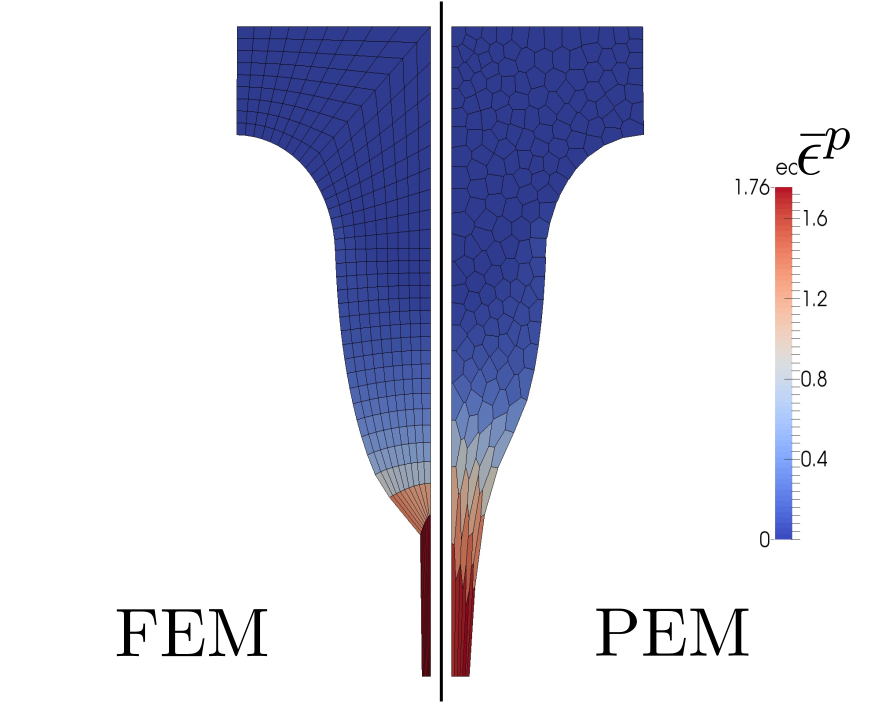
\includegraphics[width=3.0in]{figures/necking_eqps_3.pdf}
    			\caption{$t=1$ \label{fig:necking_eqps_3}}
    \end{subfigure}
    \caption{Comparison of necking behavior at various times during the analysis, depicting deformed shape, and values of equivalent plastic strain.}
\end{figure}

\subsection*{Taylor Bar Impact Problem}



For high impact velocities, the Taylor impact test under consideration is typically modeled as a coupled thermo-mechanical problem. Moreover, many finite element simulations (\cite{Heinstein:05}, \cite{Banerjee:05}) employ temperature- and strain-rate-dependent material models (such as the model of Johnson and Cook \cite{Johnson&Cook:83}). To avoid over-complicating the subsequent analyses, isothermal conditions are assumed. Additionally, the simple (rate-independent) $J_2$ elastoplasticity model described in the previous section will be used for the 

The numerical model herein sought to mimic the experimental setups detailed in \cite{Johnson&Cook:83} and \cite{Gust:82}. The impact specimen was a cylindrical billet with an initial height of 30mm, and an initial diameter of 6mm. The billet was given material properties consistent with those of OFHC copper. The following model parameters were estimated based on experimental data from \cite{Hecker:73}: the material density was specified as 8,930 kg/$\text{m}^3$, the elastic properties were taken to be $E = 110$ GPa, $\nu = 0.343$, the initial yield stress was approximated as $Y_0 = 41.37$ MPa, and the linear hardening modulus was estimated as $H = 2.3$ GPa. The billet was given an initial velocity of $400$ m/s.

Frictionless contact between the billet and the rigid surface corresponding to $X_3 = 0.0$ was modeled via the inclusion of a penalty traction of the form:
\begin{equation}
	\bar{t}_1 = \bar{t}_2 = 0, \quad \bar{t}_3 = p \langle -u_3|u_3|  \rangle,
\end{equation}
where $u_3$ corresponds to the vertical displacement of a given point on the bottom surface of the billet, and $p$ denotes a penalty stiffness parameter. For the problem at hand, an ad hoc value of $p = 6.0E+016$ was chosen, following a process of trial-and-error.

\begin{figure}[!h]
  \centering
    \begin{subfigure}[b]{0.49\linewidth}
            \centering
            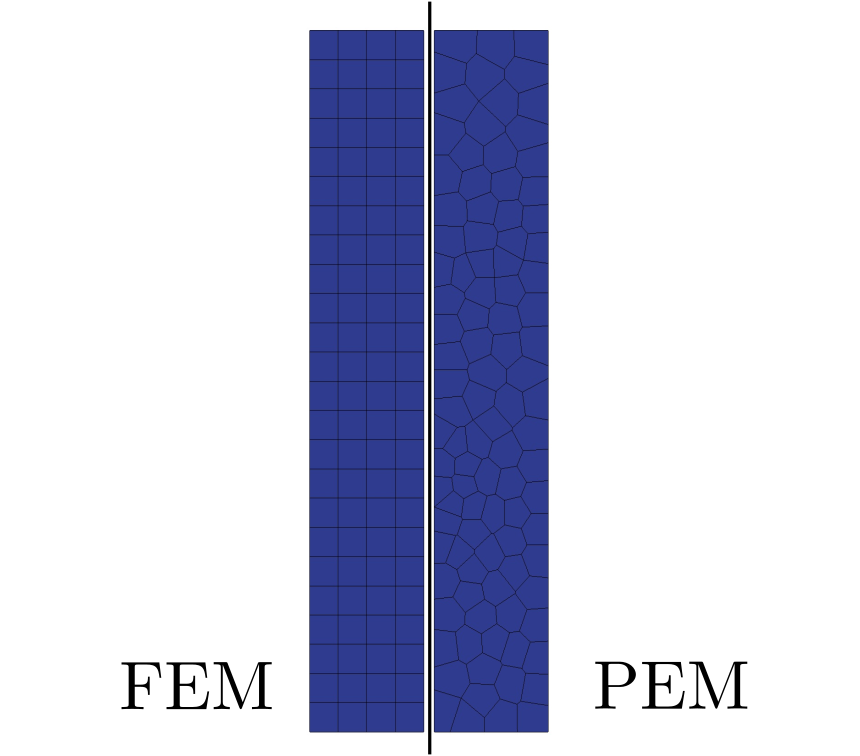
\includegraphics[width=3.0in]{figures/taylor_eqps_0.pdf}
    			\caption{$t=0.0$ \label{fig:taylor_eqps_0}}
    \end{subfigure}
	\begin{subfigure}[b]{0.49\linewidth}
            \centering
            \includegraphics[width=3.0in]{figures/taylor_eqps_1.pdf}
    			\caption{$t=1.0\times 10^{-6}$ \label{fig:taylor_eqps_1}}
    \end{subfigure} \caption{Comparison plot of the deformed shape and equivalent plastic strain $\bar{\epsilon}^p$ within the Taylor bar impact specimen.}
  \label{fig:taylor_eqps}
\end{figure}

\begin{table}[!ht]
  \begin{center}
    \begin{tabular}{| c || c | c |}
    \hline
                           & $\Delta r$ & $\Delta L$  \\ \hline \hline
    FEM                    & 0.0028075  & -0.01203919 \\ \hline
    DG-PEM ($\beta = 0.5$) & 0.0030314  & -0.01187327 \\ \hline
    DG-PEM ($\beta = 0.1$) & 0.0031577  & -0.01182747 \\
    \hline
    \end{tabular}
    \caption{Change in base width and billet length.}
    \vspace{-5pt}
    \label{tab:change_in_length_measurements}
    \vspace{-25pt}
  \end{center}
\end{table}
\chapter{Conclusions and Future Work} \label{ch:future_work}
%
Based upon the preceding investigations, the DG-PEM performs well in comparison to the classical FEM for a variety of large deformation problems. Though the DG-PEM does not directly address the issue of locking, it nonetheless provides an avenue for exploring more general discretizations which may be less sensitive to locking. Additionally, the DG-PEM demonstrates crucial improvements over the CG-PEM and the VETFEM with regard to its ability to tolerate non-convex elements, and elements with comparatively short edges.

Although some initial sensitivity analyses have been conducted for the DG-PEM with regard to the choice of penalty parameters $\alpha_{\sigma0}$, $\alpha_{\sigma1}$, a more thorough study is warranted. Particularly for the case where $\epsilon = +1$, $\alpha_{\sigma0} = \alpha_{\sigma1} = 0$ (corresponding to the OBB method \cite{Oden:98}), such settings may yield integration consistency without having to apply a gradient correction scheme. Additionally, the OBB method is provably stable for approximation spaces consisting of polynomials of order $k=2$, though this would present a challenge with regard to accurate and efficient numerical integration of quadratic polynomials.

It currently remains to be rigorously proven that the PEM yields a stable integration of the weak form for elements employing an edge-based partition and composite mid-point quadrature. Moreover, the effects of using a gradient correction scheme on high-order elements needs to be investigated further.

An exploration of the PEM for explicit dynamics applications is also warranted. Given the preliminary results that were obtained for the Taylor bar problem (using implicit dynamics), the major challenges would likely be mesh tangling and element inversion. The stable time step size for explicit analyses may present an additional challenge, being limited by the smallest dimension of any element contained in the mesh. Consequently, the inclusion of elements with short edges may negatively impact the efficiency of the computations for explicit time-stepping if random Voronoi meshes are utilized. However, considering the reasonably well-conditioned element stiffness matrices produced by the DG-PEM for elements with short edges, it may be possible to overcome some of these limitations. Further investigation is required to confirm if this is the case.

Another important consideration for the PEM in the context of non-linear solid mechanics applications is the issue of contact constraint enforcement. Particularly in 3-dimensions, the representation of a given face's shape functions (and its deformed shape) will be discontinuous if the DG-PEM is employed. Consequently, it is not clear how best to enforce contact constraints upon these discontinuous surfaces. Moreover, if the intermediary information regarding the representation of a given element face's shape functions is ultimately discarded prior to the beginning of the analysis (as suggested in \ref{ch:implementation}), then there would be no clear way to evaluate gap functions. The use of the PEM for contact applications would therefore necessitate storage of each boundary face's geometric partition. Additionally, the shape functions for these faces would need to be represented explicitly as piecewise polynomial fields.

A node-on-face method of contact enforcement would likely present a number of challenges for the DG-PEM, owing to the inherently discontinuous representation of the deformed mesh boundary. The CG-PEM may be preferred in this setting, if only for the sake of defining shape functions on element faces. In contrast, a face-on-face method may be capable of handling contact between discontinuous surfaces. Specifically, the mortar-based approach proposed in \cite{Wopschall:17} constructs a projected medial plane between each pair of contacting faces, enforcing a zero-mean gap condition between each overlapping face pair. The use of such projections may allow for the DG-PEM to be utilized directly, even if the geometric representation for each face is discontinuous.

Ongoing efforts are currently directed at improving the resistance of PEM elements to traditional forms of locking, including volumetric locking, and shear locking for thin elements. Numerous attempts were made to try to improve the bending behavior of thin elements, in particular, but these encountered various issues. An examination of enhanced strain formulations in the context of PEM may yield fruitful results. In particular, because the PEM establishes a local approximation space to construct an element's shape functions, this same space could be utilized to construct a set of enhancement functions, specific to each element.

Another issue that was given considerable attention was the subject of non-planar faces and non-linear edges. Within this setting, it suffices to say that the preservation of polynomial completeness is not a trivial matter. Various approaches to address this issue were explored, though they all invariably encountered issues of numerical precision for nearly-planar faces and nearly-linear edges, resulting in very poor interpolation errors. Most of the aforementioned investigations examined only cases where the faces/edges were represented as piecewise linear manifolds. The consideration of curved geometries (such as NURBS surfaces) would present an additional challenge.

Extending the DG-PEM approach to higher-order elements (beyond $k=2$) poses a number of practical barriers, particularly with regard to efficiency. For successively higher order elements, the size of the local DG-PEM problems arising from (\ref{eq:dgpem_linear_system}) can become large. The assembly and solution of these systems of equations will therefore impart a large computational expense for analyses with high-order elements. In such cases, solving (\ref{eq:dgpem_linear_system}) directly may be impractical. As a possible alternative, it may be sufficient to solve (\ref{eq:dgpem_linear_system}) using an iterative approach, such as the conjugate gradient method. Certain essential characteristics of the resulting solution would need to be preserved, namely: polynomial completeness, and rank sufficiency of the resulting element stiffness matrices. If successful, such an approach could greatly reduce the computational burden of the PEM shape function construction procedure.

However, the performance of any iterative solver typically depends upon the numerical conditioning of the associated linear system of equations. Poor conditioning of the DG-PEM equation systems would therefore present a major obstacle to the aforementioned approach. Even for reasonably well-scaled polynomial bases, preconditioning would likely be required to address this issue. Given the structure of the PEM, a geometric multigrid-based preconditioner could be readily obtained, though a simple Jacobi (diagonal) preconditioner might suffice. A more thorough investigation would need to be carried out to determine the efficacy of any iterative approach for constructing PEM shape functions.

Finally, an investigation into the computational efficiency of the PEM still needs to be carried out. The computational expense of the PEM shape function construction procedure should be quantified in this setting. For general polyhedral discretizations, it is expected (and informally observed for the problems considered in this work) that the classical FEM outperforms the DG-PEM on meshes with comparable numbers of elements. Two key observations may explain this behavior: in comparison to polyhedral meshes with the same number of elements, hexahedral meshes typically possess fewer nodes (degrees of freedom), and the bandwidth of the resulting global stiffness matrix tends to be smaller, as well. Moreover, elements with arbitrary topology necessitate the use of data structures with variable size, incurring an additional overhead. The FEM is therefore expected to yield better computational efficiency, in general. Nonetheless, the PEM could potentially enable the use of novel linear solution methodologies (such as geometric multigrid methods), exploiting the geometric flexibility of the elements. Such approaches could help to improve the overall efficiency of the PEM.

\appendix

\chapter{An Exact Solution for the Incompressible Twisting Annulus Problem}

An exact solution for the twisting annulus problem described in chapter \ref{ch:results} may be obtained by considering the stress divergence equations in cylindrical polar coordinates:
\begin{equation}
  \nabla \cdot \boldsymbol{\sigma} = \left\{ \begin{array}{c} \frac{\partial \sigma_{rr}}{\partial r} + \frac{\sigma_{rr}}{r} + \frac{1}{r} \frac{\partial \sigma_{\theta r}}{\partial \theta} + \frac{\partial \sigma_{z r}}{\partial z} - \frac{\sigma_{\theta \theta}}{r} \\
    \frac{1}{r} \frac{\partial \sigma_{\theta \theta}}{\partial \theta} + \frac{\partial \sigma_{r\theta}}{\partial r} + \frac{\sigma_{r\theta}}{r} + \frac{\sigma_{\theta r}}{r} + \frac{\partial \sigma_{z \theta}}{\partial z} \\
    \frac{\partial \sigma_{z z}}{\partial z} + \frac{\partial \sigma_{r z}}{\partial r} + \frac{\sigma_{r z}}{r} + \frac{1}{r} \frac{\partial \sigma_{\theta z}}{\partial \theta} \end{array} \right\} = \mathbf{0}.
\end{equation}
By the assumptions of plane strain and axisymmetry, it is rationalized that $\boldsymbol{\sigma} (r)$ must be a function of $r$, alone. Therefore:
\begin{equation}
  \nabla \cdot \boldsymbol{\sigma} = \left\{ \begin{array}{c} \frac{\partial \sigma_{rr}}{\partial r} + \frac{\sigma_{rr} - \sigma_{\theta \theta}}{r} \\
    \frac{\partial \sigma_{r\theta}}{\partial r} + \frac{2 \sigma_{r\theta}}{r} \\
    \frac{\partial \sigma_{r z}}{\partial r} + \frac{\sigma_{r z}}{r} \end{array} \right\} = \mathbf{0}.
\end{equation}
Furthermore, by the assumptions of plane strain, it is observed that $\sigma_{rz} = 0$ and $\sigma_{\theta z} = 0$. Additionally, imposing the incompressibility condition $\nabla \cdot \mathbf{v} = \text{tr} (\mathbf{D}) = 0$:
\begin{equation}
  \text{tr} (\dot{\boldsymbol{\sigma}}) = 0 \, \Rightarrow \, \text{tr} (\boldsymbol{\sigma}) = 0 \, \forall t.
\end{equation}
Suppose that $p = \sigma_{zz} = 0$, and therefore $\sigma_{\theta \theta} = - \sigma_{rr}$. This yields 2 governing differential equations for $\sigma_{rr}$ and $\sigma_{r \theta}$:
\begin{equation}
  \frac{\partial \sigma_{rr}}{\partial r} + \frac{2 \sigma_{rr}}{r} = 0, \quad \frac{\partial \sigma_{r\theta}}{\partial r} + \frac{2 \sigma_{r\theta}}{r} = 0,
\end{equation}
whose solutions are of the form
\begin{equation}
  \sigma_{rr} = \frac{\sigma}{r^2}, \quad \sigma_{r\theta} = \frac{\tau}{r^2},
\end{equation}
where $\sigma(t)$ and $\tau(t)$ are independent functions of time. Consequently,
\begin{equation}
  \left\{ \begin{array}{c} \sigma_{rr} \\ \sigma_{\theta \theta} \\ \sigma_{r \theta} \end{array} \right\} = r^{-2} \left\{ \begin{array}{c} +\sigma \\ -\sigma \\ \tau \end{array} \right\}.
\end{equation}

Under the assumption of incompressibility, the velocity field is $v_r = 0$, $v_z = 0$, and $v_\theta (r) = r \dot{\phi}(r)$, for some $\phi(r,t)$. The velocity gradient (in cylindrical polar coordinates) is written:
\begin{equation}
  \mathbf{L} = \nabla \mathbf{v} = \left[ \begin{array}{ccc} v_{r,r} & v_{r,\theta}/r-v_\theta /r & v_{r,z} \\
      v_{\theta,r} & v_{\theta,\theta}/r + v_r /r & v_{\theta,z} \\
      v_{z,r} & v_{z,\theta} /r & v_{z,z} \end{array} \right] = 
  \left[ \begin{array}{ccc} 0 & -\dot{\phi} & 0 \\
      \dot{\phi} + r \dot{\phi}_{,r} & 0 & 0 \\
      0 & 0 & 0 \end{array} \right].
\end{equation}
The corresponding rate of deformation and spin tensors are:
\begin{equation}
  \mathbf{D} = \frac{r \dot{\phi}_{,r}}{2} \left[ \begin{array}{ccc} 0 & +1 & 0 \\
      +1 & 0 & 0 \\
      0 & 0 & 0 \end{array} \right], \quad \mathbf{W} = 
  \frac{2 \dot{\phi} + r \dot{\phi}_{,r}}{2} \left[ \begin{array}{ccc} 0 & - 1 & 0 \\
      +1 & 0 & 0 \\
      0 & 0 & 0 \end{array} \right].
\end{equation}
The stress rate equations resulting from $\dot{\boldsymbol{\sigma}} = \mathbb{C} : \mathbf{D} + \mathbf{W} \boldsymbol{\sigma} - \boldsymbol{\sigma} \mathbf{W}$ are
\begin{equation}
  \left\{ \begin{array}{c} \dot{\sigma}_{rr} \\ \dot{\sigma}_{\theta \theta} \\ \dot{\sigma}_{r \theta} \end{array} \right\} = \left\{ \begin{array}{c} 0 \\ 0 \\ \mu r \dot{\phi}_{,r} \end{array} \right\} + 
  (2 \dot{\phi} + r \dot{\phi}_{,r}) \left\{ \begin{array}{c} - \sigma_{r \theta} \\ \sigma_{r \theta} \\ \sigma_{rr} \end{array} \right\},
\end{equation}
or (in terms of $\sigma$, $\tau$):
\begin{equation}
  \left\{ \begin{array}{c} \dot{\sigma} \\ \dot{\tau} \end{array} \right\} = \left\{ \begin{array}{c} 0 \\ \mu r^3 \dot{\phi}_{,r} \end{array} \right\} + (2 \dot{\phi} + r \dot{\phi}_{,r}) \left[ \begin{array}{cc} 0 & -1 \\ 1 & 0 \end{array} \right] \left\{ \begin{array}{c} \sigma \\ \tau \end{array} \right\},
\end{equation}
which must be valid for all $r, \, t$. Assume that $\dot{\phi}(r)$ is a function of $r$ (and not of $t$), corresponding to a steady rate of deformation. By recognizing that $\sigma_{,r} = \tau_{,r} = 0$, one obtains the condition
\begin{equation}
  3 \dot{\phi}_{,r} + r \dot{\phi}_{,rr} = 0,
\end{equation}
implying $\dot{\phi}_{,r} = B r^{-3}$, and $\phi (r, t) = (A - B r^{-2} / 2)t$. Thus
\begin{equation}
  \left\{ \begin{array}{c} \dot{\sigma} \\ \dot{\tau} \end{array} \right\} = \left\{ \begin{array}{c} 0 \\ \mu B \end{array} \right\} + 2 A \left[ \begin{array}{cc} 0 & -1 \\ 1 & 0 \end{array} \right] \left\{ \begin{array}{c} \sigma \\ \tau \end{array} \right\},
\end{equation}
and
\begin{equation}
  \sigma(t) = - \frac{\mu B}{2 A} - C_2 \sin (2 A t) + C_1 \cos (2 A t),
\end{equation}
\begin{equation}
  \tau(t) = C_1 \sin (2 A t) + C_2 \cos (2 A t).
\end{equation}
Imposing the initial conditions $\sigma(0) = \tau(0) = 0$ results in:
\begin{equation}
  \sigma(t) = \frac{\mu B}{2 A} \left[ \cos (2 A t) - 1 \right], \quad \tau(t) = \frac{\mu B}{2 A} \sin (2 A t).
\end{equation}
Imposing the boundary conditions $\phi(R_i,t) = 0 \, \, \forall t$, $\phi(R_o,t) = \Phi \, t \, \, \forall t$ yields:
\begin{equation}
  A = \frac{R_o^{2}}{R_o^{2} - R_i^{2}} \Phi, \quad B = 2 \frac{R_o^{2} R_i^{2}}{R_o^{2} - R_i^{2}} \Phi.
\end{equation}
The final analytical solutions for the displacement and stress fields are:
\begin{equation}
  u_r = u_z = 0, \quad u_\theta = \frac{R_o^2}{r} \frac{r^2 - R_i^2}{R_o^{2} - R_i^{2}} \Phi t,
\end{equation}
\begin{equation}
  \sigma_{rr} = - \sigma_{\theta \theta} = \mu \frac{R_i^{2}}{r^{2}} \left[ \cos \left( 2 \frac{R_o^{2}}{R_o^{2} - R_i^{2}} \Phi t \right) - 1 \right], \quad \sigma_{r \theta} = \mu \frac{R_i^{2}}{r^{2}} \sin \left( 2 \frac{R_o^{2}}{R_o^{2} - R_i^{2}} \Phi t \right).
\end{equation}
According to \cite{Brannon:11}, the above solution for $\sigma_{r \theta}$ is also valid for compressible elastic materials.

\bibliography{bibliography}

%% The UMI abstract uses square brackets!
%\UMIabstract[This work presents a novel polytopal finite-element framework that addresses the collective issues of discretization sensitivity and mesh generation for computational solid mechanics problems. The use of arbitrary polygonal and polyhedral shapes in place of canonical isoparametric elements seeks to remediate issues pertaining to meshing and mesh quality (particularly for irregularly shaped elements), while maintaining many of the desirable features of a traditional finite element method.
%	
%	A general class of \textit{partitioned element methods} (PEM) is proposed and analyzed, constituting a family of approaches for constructing piecewise polynomial approximations to harmonic shape functions on arbitrary polytopes. Such methods require a geometric partition of each element, and under certain conditions will directly yield integration consistency. Two partitioned element methods are explored in detail, including a novel approach herein referred to as the \textit{discontinuous Galerkin partitioned-element method} (DG-PEM). An implementational framework for the DG-PEM is presented, along with a discussion of its associated numerical challenges.
%	
%	The numerical precision of the PEM is explored via classical patch tests and single element tests for a representative sampling of polygonal element shapes. Solution sensitivity with respect to element shape is examined for a handful of problems, including a mesh convergence study in the nearly incompressible regime. Finally, the efficacy of the DG-PEM is assessed for a number of benchmark problems involving large deformations and nonlinear material behavior.]

\end{document} 
